\documentclass[12pt,a4paper]{article}
\usepackage[utf8]{inputenc}

\usepackage{amsmath}
\usepackage{amsfonts}
\usepackage{amssymb}
\usepackage{graphicx}
\usepackage{listings}
\usepackage[margin=1.0in]{geometry}
\usepackage{caption}
\usepackage{subcaption}
\usepackage{float}
\usepackage[utf8]{inputenc}
\usepackage{refstyle}
\usepackage{spverbatim}
\usepackage{listings}
\usepackage{csvsimple}
\usepackage{adjustbox}
\usepackage{cancel}
\usepackage{scalerel,stackengine}
\stackMath
\newcommand\reallywidehat[1]{%
\savestack{\tmpbox}{\stretchto{%
  \scaleto{%
    \scalerel*[\widthof{\ensuremath{#1}}]{\kern-.6pt\bigwedge\kern-.6pt}%
    {\rule[-\textheight/2]{1ex}{\textheight}}%WIDTH-LIMITED BIG WEDGE
  }{\textheight}% 
}{0.5ex}}%
\stackon[1pt]{#1}{\tmpbox}%
}
\parskip 1ex

\lstset{numbers=left,
	title=\lstname,
	numberstyle=\tiny, 
	breaklines=true,
	tabsize=4,
	language=Python,
	morekeywords={with,super,as},,
	frame=single,
	basicstyle=\footnotesize\tt,
	commentstyle=\color{comment},
	keywordstyle=\color{keyword},
	stringstyle=\color{string},
	backgroundcolor=\color{background},
	showstringspaces=false,
	numbers=left,
	numbersep=5pt,
	literate=
		{æ}{{\ae}}1
		{å}{{\aa}}1
		{ø}{{\o}}1
		{Æ}{{\AE}}1
		{Å}{{\AA}}1
		{Ø}{{\O}}1
	}

\usepackage{bm}
\usepackage{hyperref}
\usepackage[usenames, dvipsnames]{color}

\begin{document}

\begin{center}
\LARGE{\textbf{Project 1: Regression analysis and resampling methods}}
\\
\large{\textbf{Course: FYS-STK4155}}
\\
\large{\textbf{Semester: Autumn 2020}}
\\
\large{\textbf{Name: Sander Losnedahl}}
\end{center}

\begin{center}
\Large{\textbf{Abstract}}
\end{center}

\noindent This project first develops the OLS regression scheme in order to predict the Franke function. This is done successfully and the predictive capabilities of the OLS model is then studied when the number of observations and the noise-level is varied. It is observed that the number of observations does matter, at least to a certain extent. Therefore, resampling methods in the form of bootstrapping and cross-validation is introduced in order to increase the number of observations to a certain level. These resampling methods then makes the prediction by the OLS regression scheme better. Shrinkage methods in form of Ridge and Lasso is then introduced which in combination with the resampling methods are also able to accurately predict the Franke function. Lastly, real terrain data is introduced and the developed regression schemes and resampling methods are shown to be able to somewhat predict this new terrain data. The algorithms are able to capture the overarching traits of the real terrain data, but lacks the attention to detail. It is also found that Ridge regression performs the best on the real data out of the three regression schemes.

\newpage

\begin{center}
\Large{\textbf{Introduction}}
\end{center}

\noindent The main goal of this report is to create linear regression schemes that trains a model based on data followed by a prediction of the trained model. The prediction is the models capability to infer information on data the model has never seen before. Such algorithms are within the realm of machine learning and has numerous real world applications. However, before real data can be introduced, synthetic data will be used in order to ensure the regression schemes work properly. The synthetic data in question is the Franke function, which is a weighted sum of exponentials and it will act as the response for the regression scheme to train on. The variables used in the training will be polynomials of different orders and also combinations of these polynomials.
\\
The first regression scheme will be the ordinary least squares which tries to predict a response based on minimizing the residual sum of squares. After the ordinary least squares is implemented, I introduce shrinkage methods in the form of Ridge and Lasso. This methods also aim to minimize the residual sum of squares, but additionally aim to reduce variables (different order polynomials) towards/to zero. The resulting predictions from the shrinkage methods will then be compared to the ordinary least squares. 
\\
The above mentioned regression schemes often rely on large amounts of data to train on. This may cause a problem as large amounts of data is not always available in the real world. Therefore, resampling methods are introduced to "create data our of thin air". I here experiment with two different types of resampling methods, namely the bootstrap and cross-validation methods.
\\
When the three regression schemes are implemented alongside the resampling methods, I introduce real terrain data from Norway. The same algorithms used to predict the Franke function will then be applied to the real data, and hopefully the results will be reasonable.

\newpage

\begin{center}
\Large{\textbf{Preliminaries}}
\end{center}

\noindent \textbf{The github page} can be found at \href{{https://github.com/sanderwl/FYS-STK4155}}{\nolinkurl{https://github.com/sanderwl/FYS-STK4155}} under the folder "project 1". Here you can find the python code used to generate the results in this report as well as the report itself with figures and data.
\\
\textbf{Scaling the data} is necessary in order to make sense of the output values. If the data is unscaled, the resulting numbers will not make much sense as we have no reference to what are low and high numbers. When we scale the data we subtract the sample mean and divide by the sample standard deviation of the data, we essentially make the data centred around zero with standard deviation one. This way, we always have a reference to the outcome as it is always relative to zero. Additionally, most regression algorithms rely on the data having lower distance between the data points, making scaling an important pre-processing step.
\\
\textbf{Noise level} is a recurrent theme throughout this report. Noise is added to the data (exercises a-e) in order to prepare for the real data later on. The noise that is added has a standard normal distribution with standard deviation $1$ and maximum value of $1$ at its mean of zero. This noise is then multiplied with a constant ($0.001$ in most cases in this report) in order to adjust the noise level. 
\\
\textbf{The train/test split} will be $75/25$ in this project. When performing regression, we need to train the algorithm using the training set, as well as validate the trained algorithm using the independent test set. There is no set ratio which is considered the best, but the training set should include the majority of the observations. 

\newpage

\begin{center}
\Large{\textbf{Exercise 1a): Ordinary least squares with changes in parameters.}}
\end{center}

\begin{center}
\large{\textbf{Ordinary least squares and its coefficients}}
\end{center}

\noindent The goal for this part of the exercise is trying to fit a linear model (linear in terms of regression coefficients) to the Franke function given as

\begin{equation}\label{eq:Franke}
\begin{aligned}
f(x,y) &= \frac{3}{4}\exp{\left(-\frac{(9x-2)^2}{4} - \frac{(9y-2)^2}{4}\right)}+\frac{3}{4}\exp{\left(-\frac{(9x+1)^2}{49}- \frac{(9y+1)}{10}\right)} \\
&+\frac{1}{2}\exp{\left(-\frac{(9x-7)^2}{4} - \frac{(9y-3)^2}{4}\right)} -\frac{1}{5}\exp{\left(-(9x-4)^2 - (9y-7)^2\right) }
\end{aligned}
\end{equation}

\noindent where polynomial combinations of x and y in the span $x,y \in [0,1]$ will be the explanatory variables. We can express a linear model using ordinary least squares as seen in equation \ref{eq:LinReg} (Hastie, T., et al.,2009, [A])

\begin{equation}\label{eq:LinReg}
\begin{aligned}
\reallywidehat{f(x,y)} = \hat{y} = \textbf{X} \boldsymbol{\beta + \epsilon}
\end{aligned}
\end{equation}

\noindent where $\reallywidehat{f(x,y)}$ or $\hat{y}$ is the least squares estimate of the Franke function, $\textbf{X}$ is the $n\times p$ design matrix consisting of the aforementioned polynomial combinations of x and y, $\boldsymbol{\beta}$ are the $p\times 1$ regression coefficients and $\boldsymbol{\epsilon}$ is just random noise/unobserved random variables. In order to get the best estimate for the Franke function, we want to choose $\boldsymbol{\beta}$-values so that we minimize the residual sum of squares (thereby the name "least squares"). Solving equation \ref{eq:LinReg} with the intent to minimize the residual sum of squares yields the estimates for the $\boldsymbol{\beta}$-values (Hastie, T., et al., [A])

\begin{equation}\label{eq:minBeta}
\begin{aligned}
\hat{\boldsymbol{\beta}} = (\textbf{X}^T\textbf{X})^{-1}\textbf{X}^T \hat{y}
\end{aligned}
\end{equation}

\noindent where T marks the transpose of the matrix. We can now get the estimate $\hat{\boldsymbol{\beta}}$ with equation \ref{eq:minBeta} and then compute the estimate of the Franke function using equation \ref{eq:LinReg}.
\\
We now turn to implementing the regression algorithm where we start by selecting a low number of observations of $n = 10$, a polynomial degree of $p = 5$ and a noise level of $0.001$. We start by creating the design matrix using polynomials of x and y (and their combinations) of degrees up to 5, scale the data, split the data and the design matrix into training and test sets with ratio $75/25$ and lastly estimate the regression coefficients using equation \ref{eq:minBeta} and calculate the estimated Franke function using equation \ref{eq:LinReg}. It is not always certain which values of beta coefficients minimize the residual sum of squares, so some uncertainty is always present. Therefore, we need to find which coefficients are uncertain, and which are certain. We quantify the uncertainty by using confidence intervals around the coefficients such that our uncertainty is within one standard deviation of the coefficient. We find said standard deviation by taking the square root of the diagonal elements of the covariance matrix (Fahrmeir, L., et al., 2013)

\begin{equation}\label{eq:diagCOV}
\begin{aligned}
\sigma = \sqrt{diag((\textbf{X}^T\textbf{X})^{-1}S^2)}
\end{aligned}
\end{equation}

\noindent where \textbf{X} is the design matrix and S is the sample variance of the response. By then taking $\beta_i \pm \sigma_i$ we can find the confidence interval of the regression coefficients which is plotted in figure \ref{fig:betaIntALL1}

\begin{figure}[H]
\centering
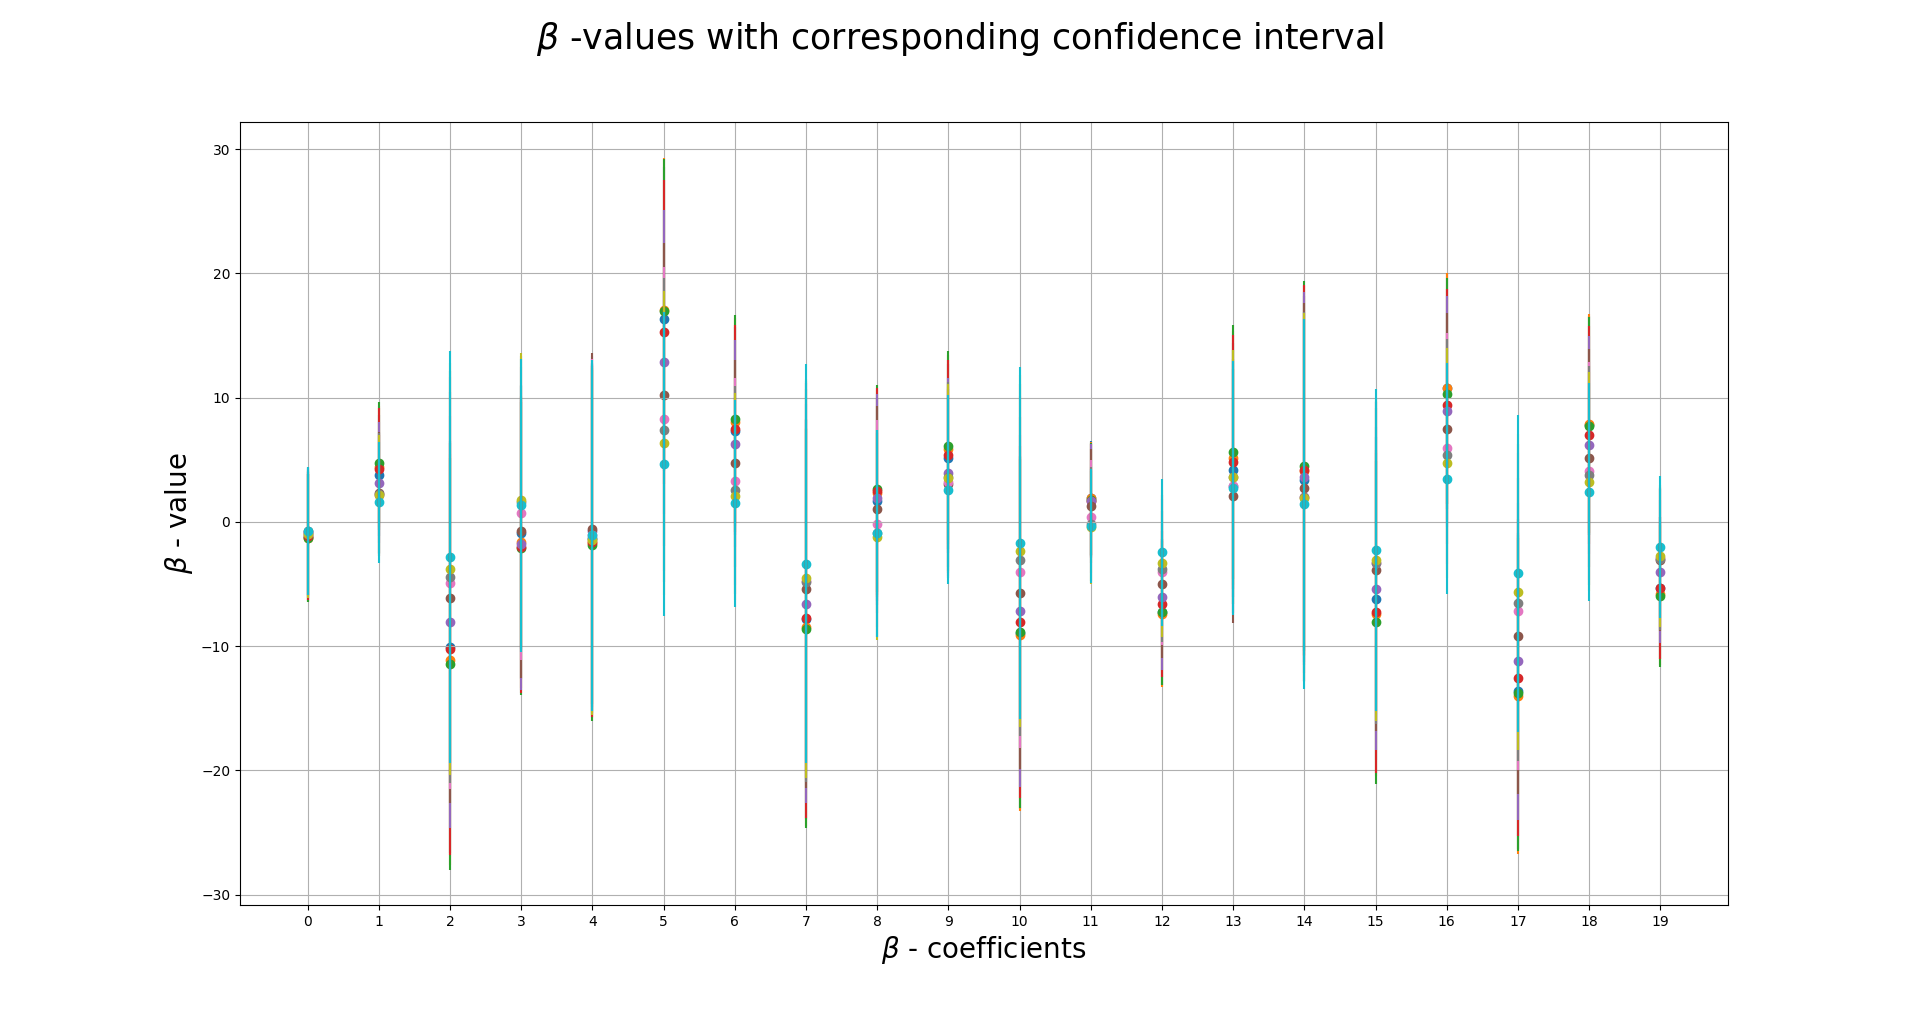
\includegraphics[width = 1\linewidth]{C:/Users/Sander/Documents/GitHub/FYS-STK4155/Project1/Report/Figures/betaInterval_ALL_n10_p5_noise0001_ts025XD.PNG}
\caption{\label{fig:betaIntALL1} $\hat{\boldsymbol{\beta}}$-coefficients from performing ordinary least squares regression. Dots indicate the actual $\hat{\boldsymbol{\beta}}$-coefficients value while bars around indicate the confidence interval ($\pm \sigma$).}
\end{figure}

\noindent Since the response is the Franke function (a matrix), we get p times n regression coefficients as seen in figure \ref{fig:betaIntALL1}. However, one can still observe from figure \ref{fig:betaIntALL1} that some regression coefficients are more certain than others. We can also plot one slice of the p times n regression coefficient matrix to get a better view as seen in figure \ref{fig:betaIntROW1}

\begin{figure}[H]
\centering
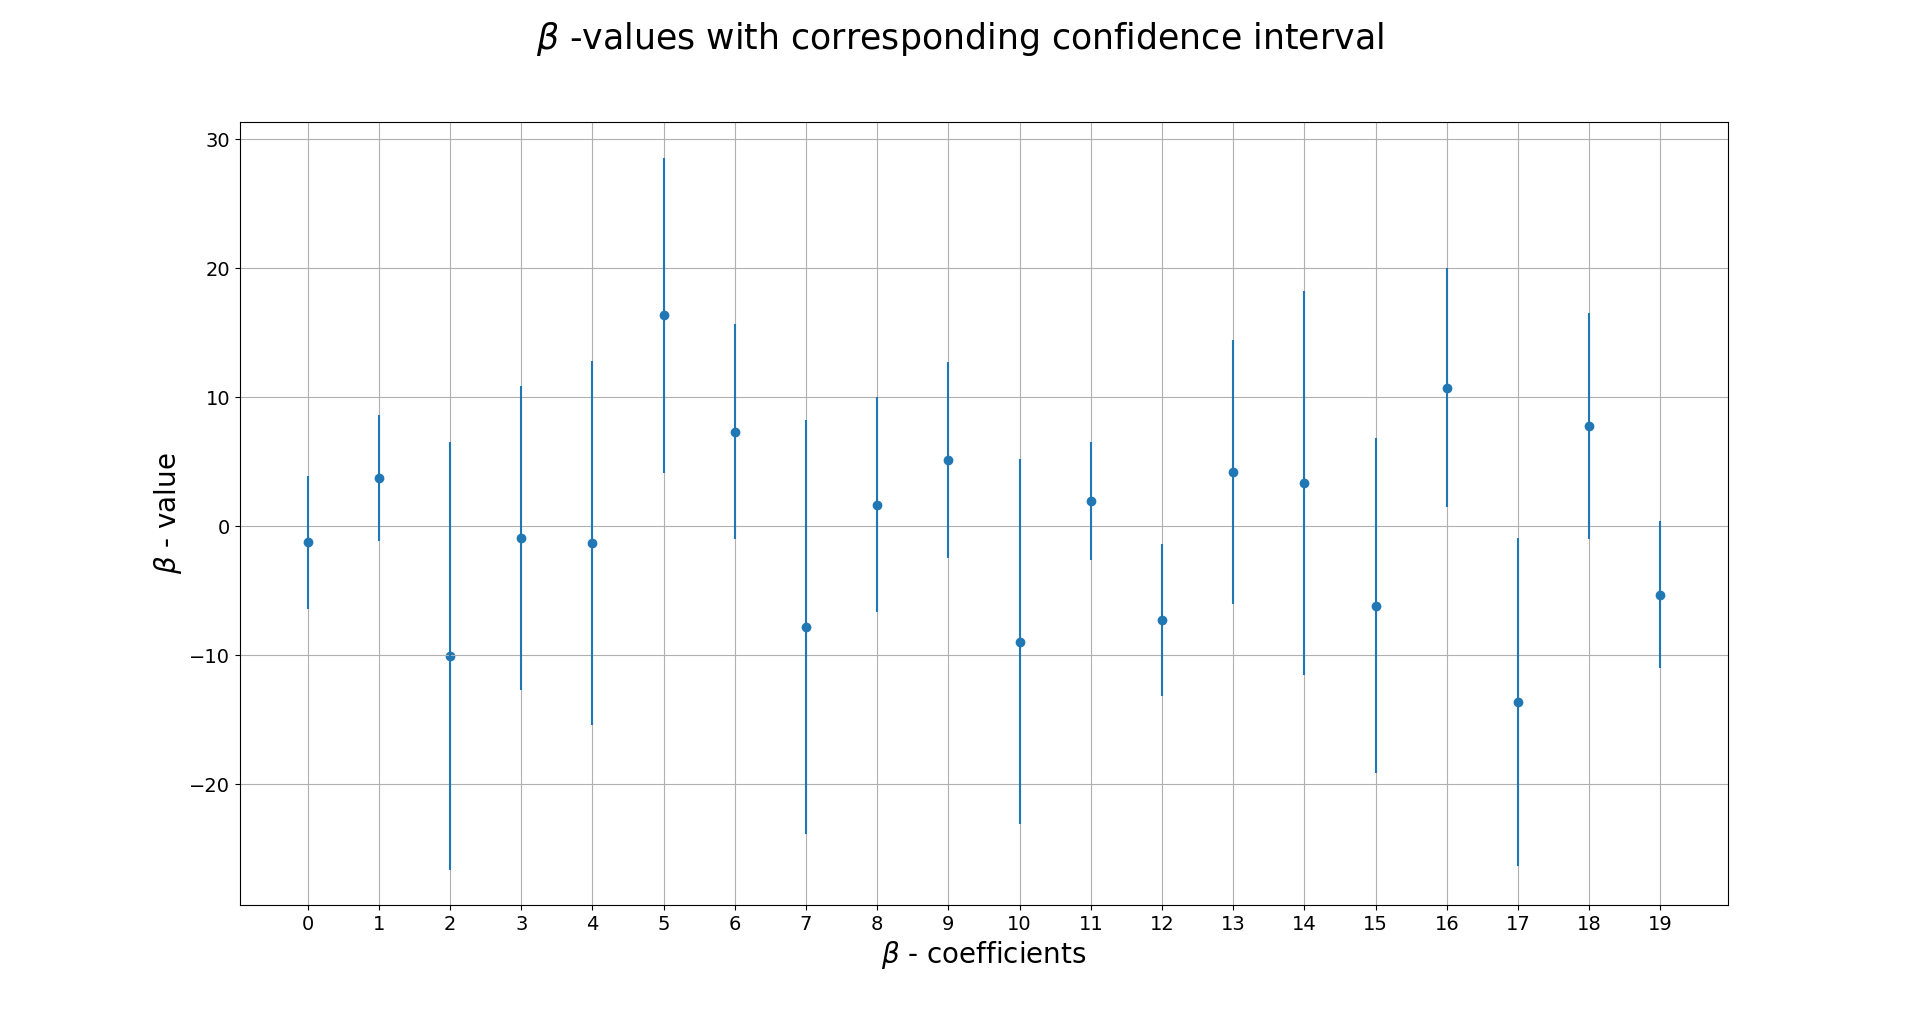
\includegraphics[width = 1\linewidth]{C:/Users/Sander/Documents/GitHub/FYS-STK4155/Project1/Report/Figures/betaInterval_1row_n10_p5_noise0001_ts025XD.PNG}
\caption{\label{fig:betaIntROW1} A slice of the $\hat{\boldsymbol{\beta}}$-coefficients from performing ordinary least squares regression. Dots indicate the actual $\hat{\boldsymbol{\beta}}$-coefficients value while bars around indicate the confidence interval ($\pm \sigma$).}
\end{figure}

\noindent As previously mentioned, some regression coefficients have relatively small confidence interval while others have larger. This means that some coefficients are more trustworthy than other. Even though the confidence interval may be large, it does not mean that particular coefficient is not responsible for explaining the response $\hat{y}$.

\begin{center}
\large{\textbf{Ordinary least squares regression on the Franke data using different parameters}}
\end{center}

\noindent Now that we have calculated and gained some faith in our regression coefficient estimates, we can utilize equation \ref{eq:LinReg} to find $\hat{y}$ which is plotted together with the real Franke function in figures \ref{fig:FrankeReal1} and \ref{fig:FrankeEst1}

\begin{figure}[H]
\centering
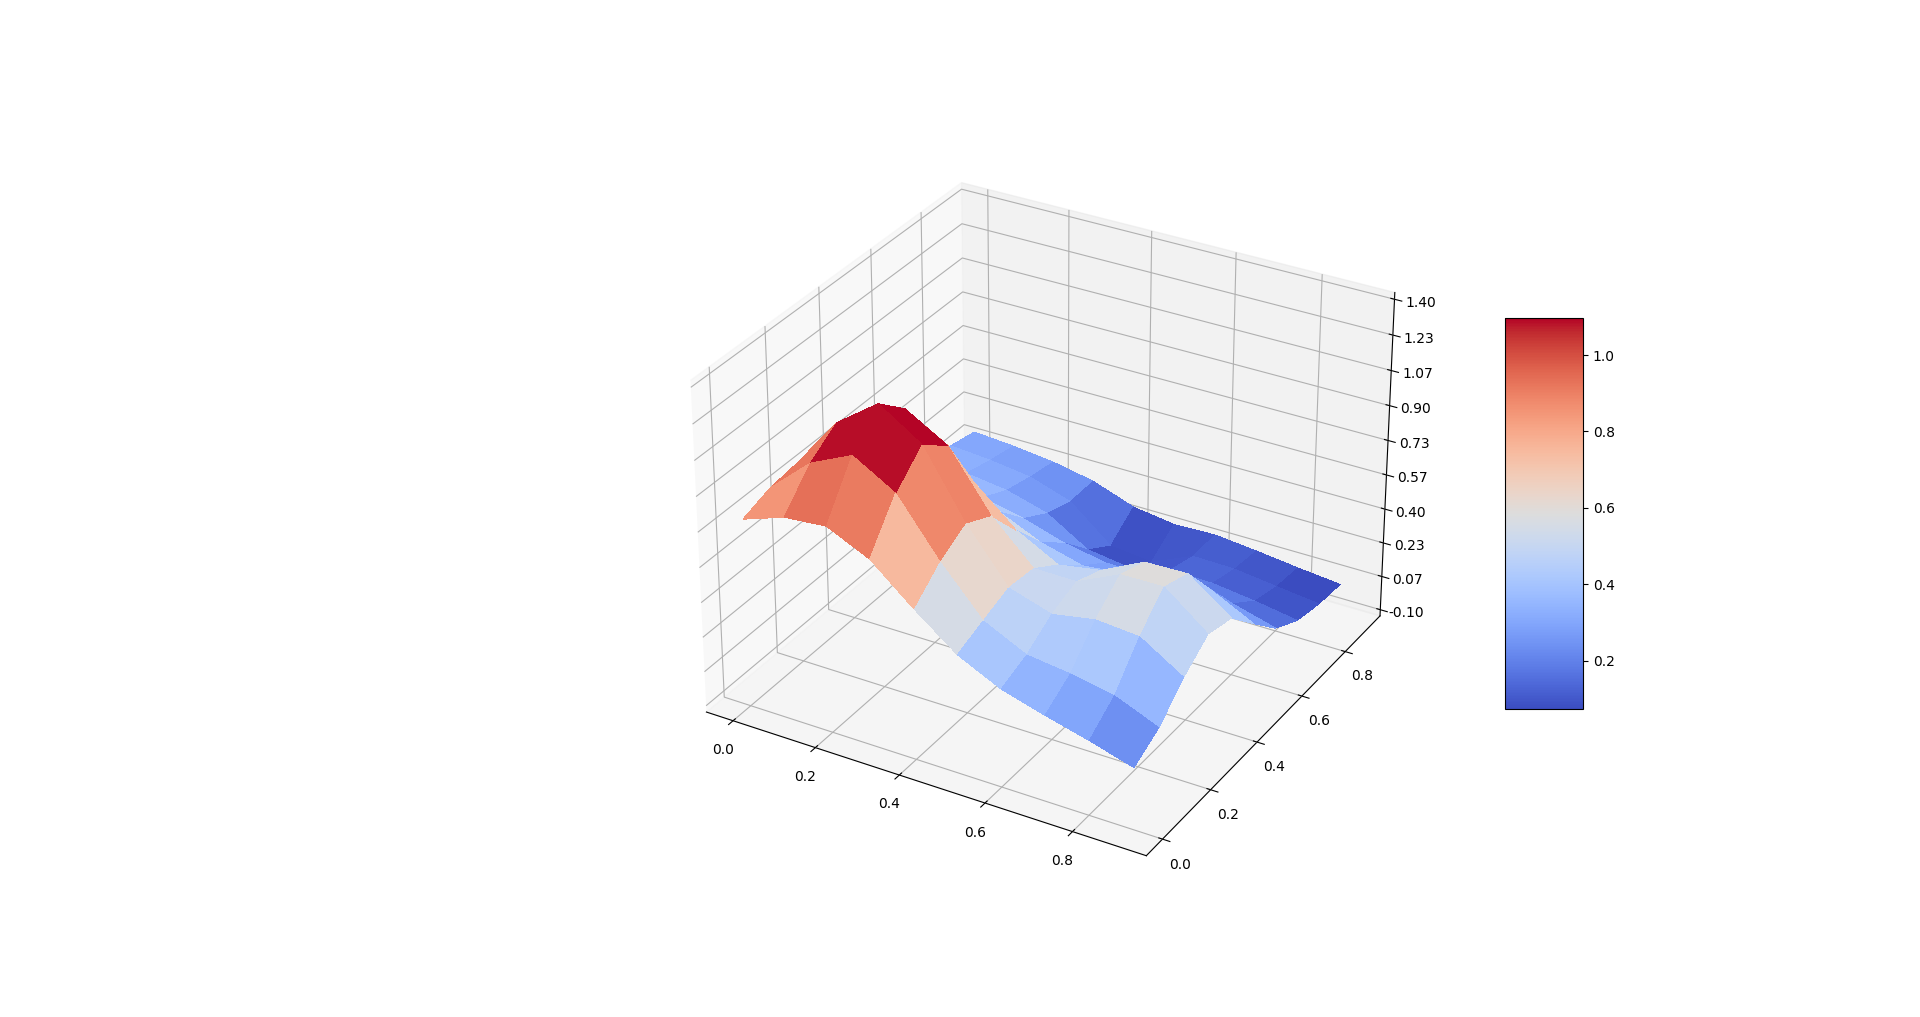
\includegraphics[width = 1\linewidth]{C:/Users/Sander/Documents/GitHub/FYS-STK4155/Project1/Report/Figures/zReal_n10_p5_noise0001_ts025.PNG}
\caption{\label{fig:FrankeReal1} The real Franke function when we have $10$ observations and polynomials of degree $5$ using a noise-level of $0.001$ and a $75/25$ train/test split.}
\end{figure}

\begin{figure}[H]
\centering
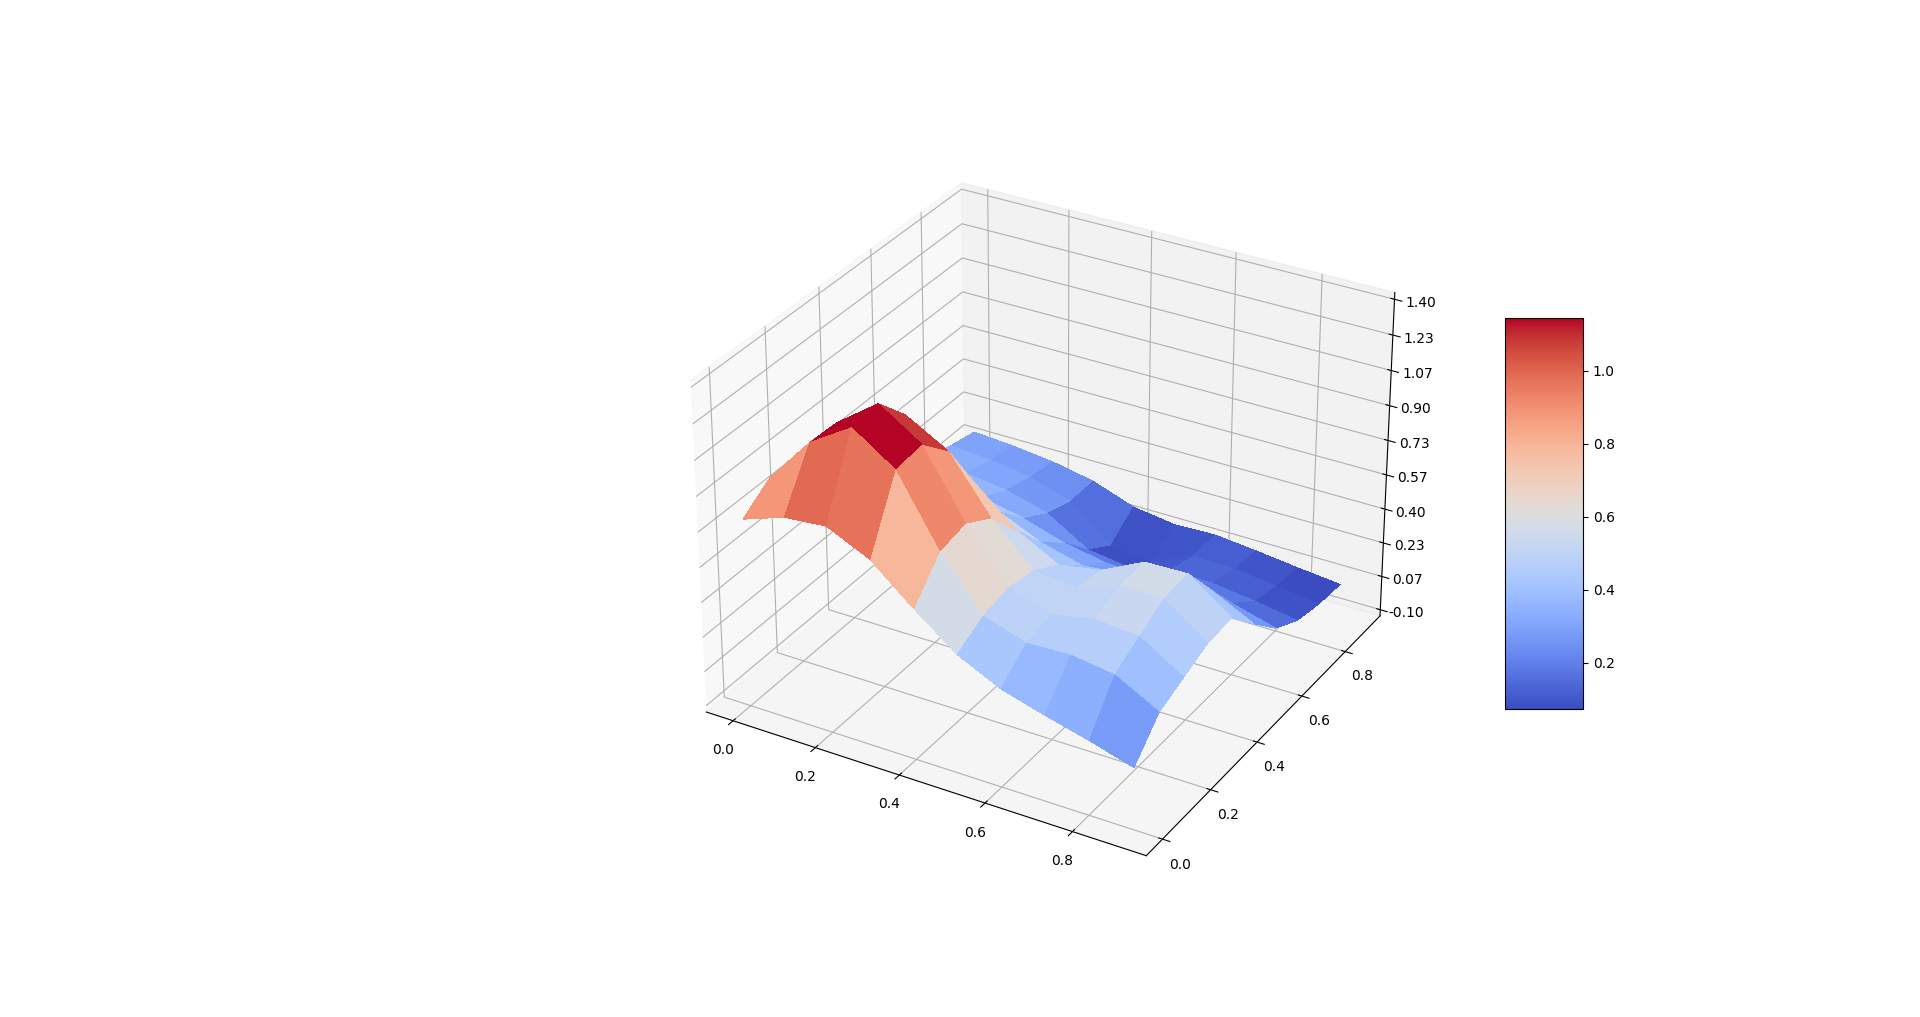
\includegraphics[width = 1\linewidth]{C:/Users/Sander/Documents/GitHub/FYS-STK4155/Project1/Report/Figures/zEst_n10_p5_noise0001_ts025.PNG}
\caption{\label{fig:FrankeEst1} The estimated Franke function when we have $10$ observations and polynomials of degree $5$ using a noise-level of $0.001$ and a $75/25$ train/test split.}
\end{figure}

\noindent It can be observed from figures \ref{fig:FrankeReal1} and \ref{fig:FrankeEst1} that our estimate is pretty good, any we can plot the difference between the two to strengthen our faith in the model

\begin{figure}[H]
\centering
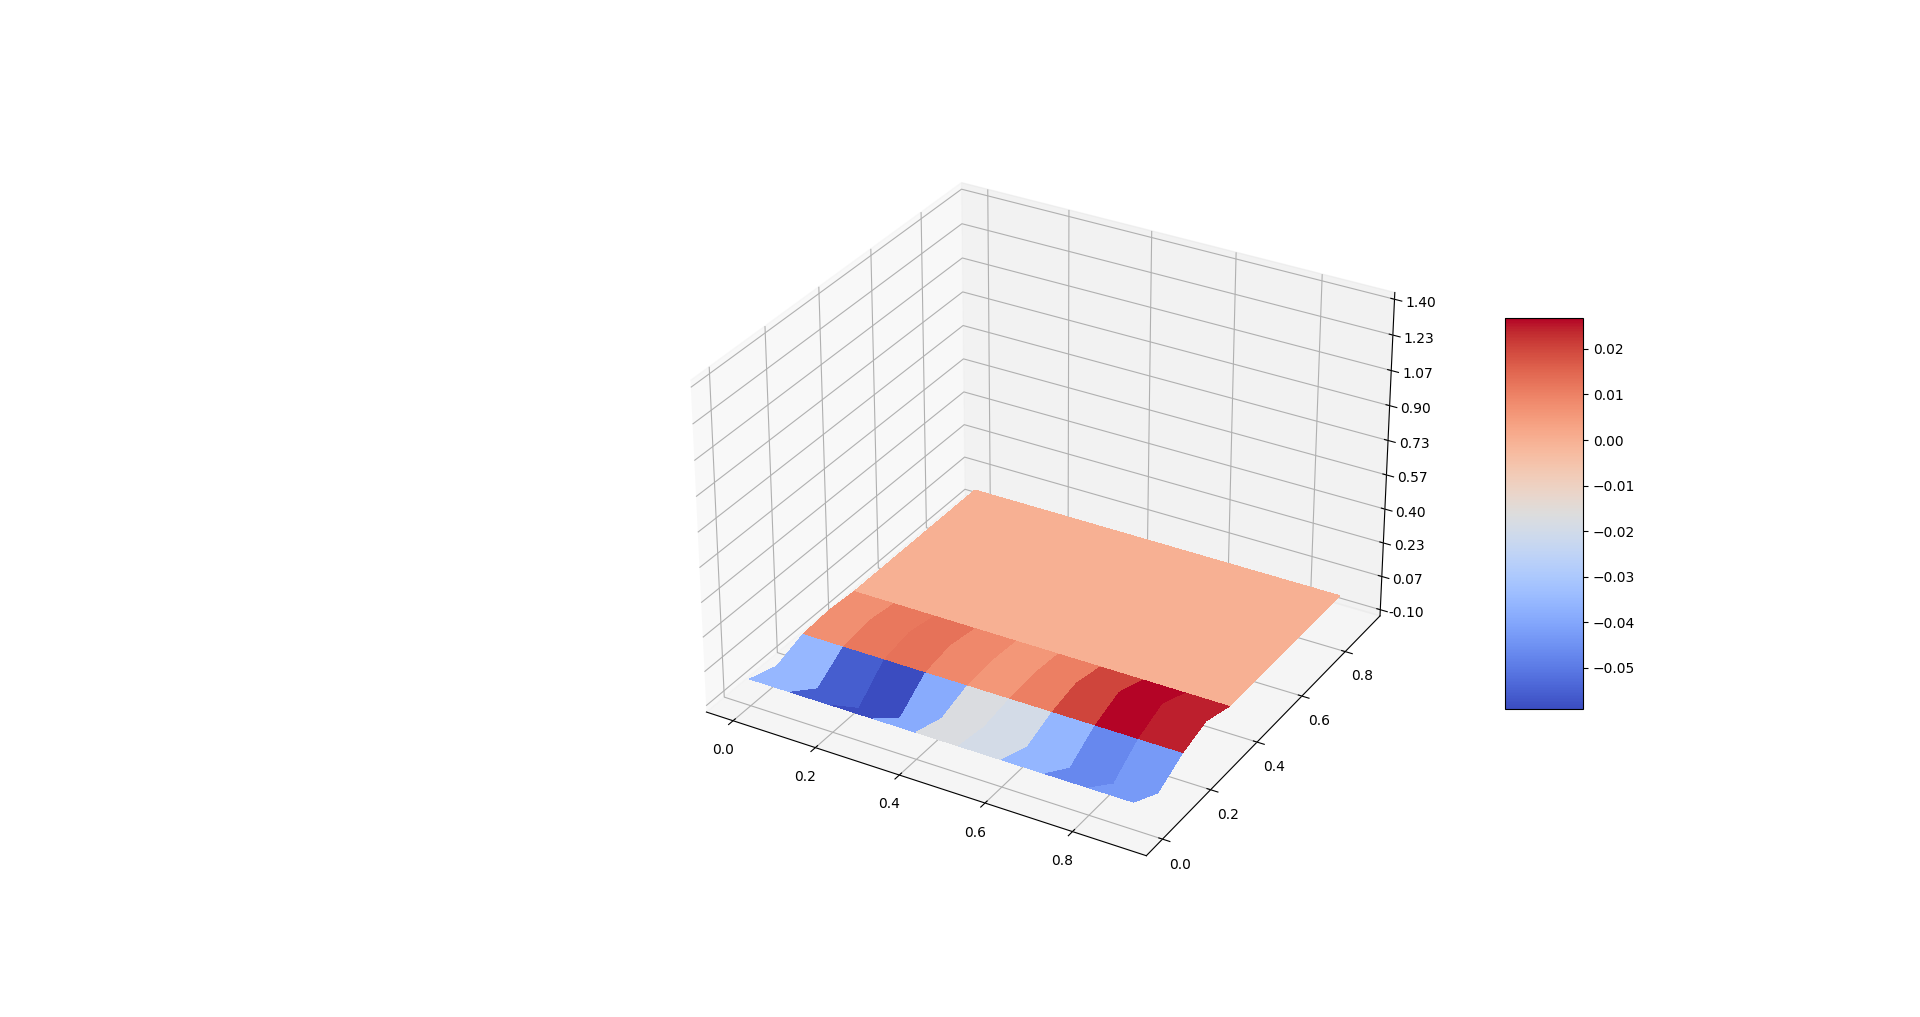
\includegraphics[width = 1\linewidth]{C:/Users/Sander/Documents/GitHub/FYS-STK4155/Project1/Report/Figures/zDiff_n10_p5_noise0001_ts025.PNG}
\caption{\label{fig:FrankeDIFF1} The difference between the real and estimated Franke functions when we have $10$ observations and polynomials of degree $5$ using a noise-level of $0.001$ and a $75/25$ train/test split.}
\end{figure}

\noindent As expected, the difference shown in figure \ref{fig:FrankeDIFF1} is very small. However, we have yet to quantified how small. This can be done using the mean square error (MSE) and $R^2$ which is calculated from equations \ref{eq:MSE} and \ref{eq:R2}

\begin{equation}\label{eq:MSE}
\begin{aligned}
MSE = \frac{1}{n} \sum_{i=0}^{n-1}(y_i-\hat{y}_i)^2
\end{aligned}
\end{equation}

\begin{equation}\label{eq:R2}
\begin{aligned}
R^2 = 1- \frac{\sum_{i=0}^{n-1}(y_i-\hat{y}_i)^2}{\sum_{i=0}^{n-1}(y_i-\bar{y}_i)^2}
\end{aligned}
\end{equation}

\noindent where $\bar{y}_i$ is the mean value of the Franke function. The MSE gives us a value of how far our estimate falls from the real Franke function, while the $R^2$ gives us how strong the relationship is between the real Franke function and our estimate. When utilizing equations \ref{eq:MSE} and \ref{eq:R2} on the data shown in figures \ref{fig:FrankeReal1} and \ref{fig:FrankeEst1} we get the values in table \ref{tab:ESTREAL1}

\begin{table}[h]
\caption{\label{tab:ESTREAL1} MSE and $R^2$ between the real and estimated Franke function when we have $10$ observations and polynomials of degree $5$ using a noise-level of $0.001$ and a $75/25$ train/test split.}
\centering
\begin{tabular}{c|c|c}
 & MSE & $R^2$\\
\hline
Training & $5.977257880702667 \times 10^{-24}$ & $1.0$\\
\hline
Test & $0.048290833950696326$ & $0.5437287443341614$\\	  
\end{tabular}
\end{table}

\noindent It should be obvious that the training set performs better than the test set, as it is the training data that is used to fit the model, particularly when n is small. So what happens when we increase the number of observations to say $n = 100$? Figures \ref{fig:FrankeReal2} , \ref{fig:FrankeEst2} and \ref{fig:FrankeDIFF2} show again the real, estimated and differential Franke functions with the same exact parameters, except for n, which is now equal to $100$

\begin{figure}[H]
\centering
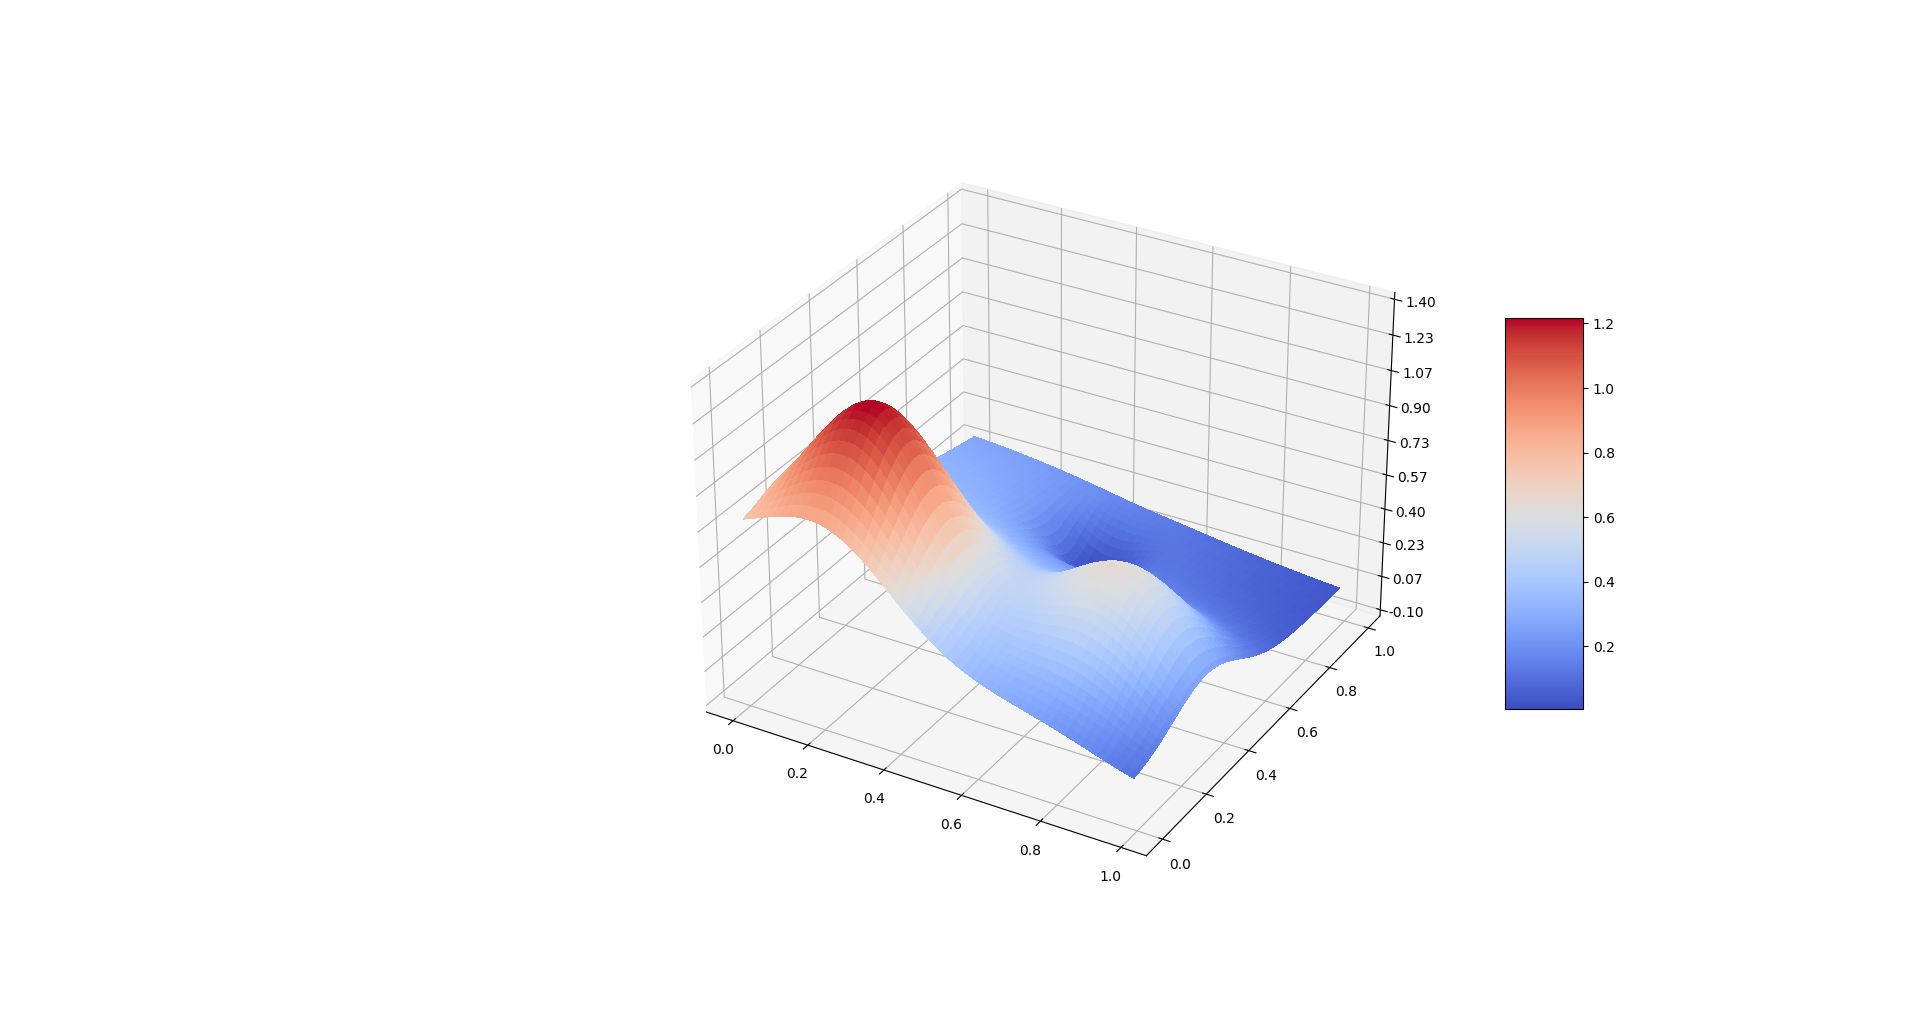
\includegraphics[width = 1\linewidth]{C:/Users/Sander/Documents/GitHub/FYS-STK4155/Project1/Report/Figures/zReal_n100_p5_noise0001_ts025.PNG}
\caption{\label{fig:FrankeReal2} The real Franke function when we have $100$ observations and polynomials of degree $5$ using a noise-level of $0.001$ and a $75/25$ train/test split.}
\end{figure}

\begin{figure}[H]
\centering
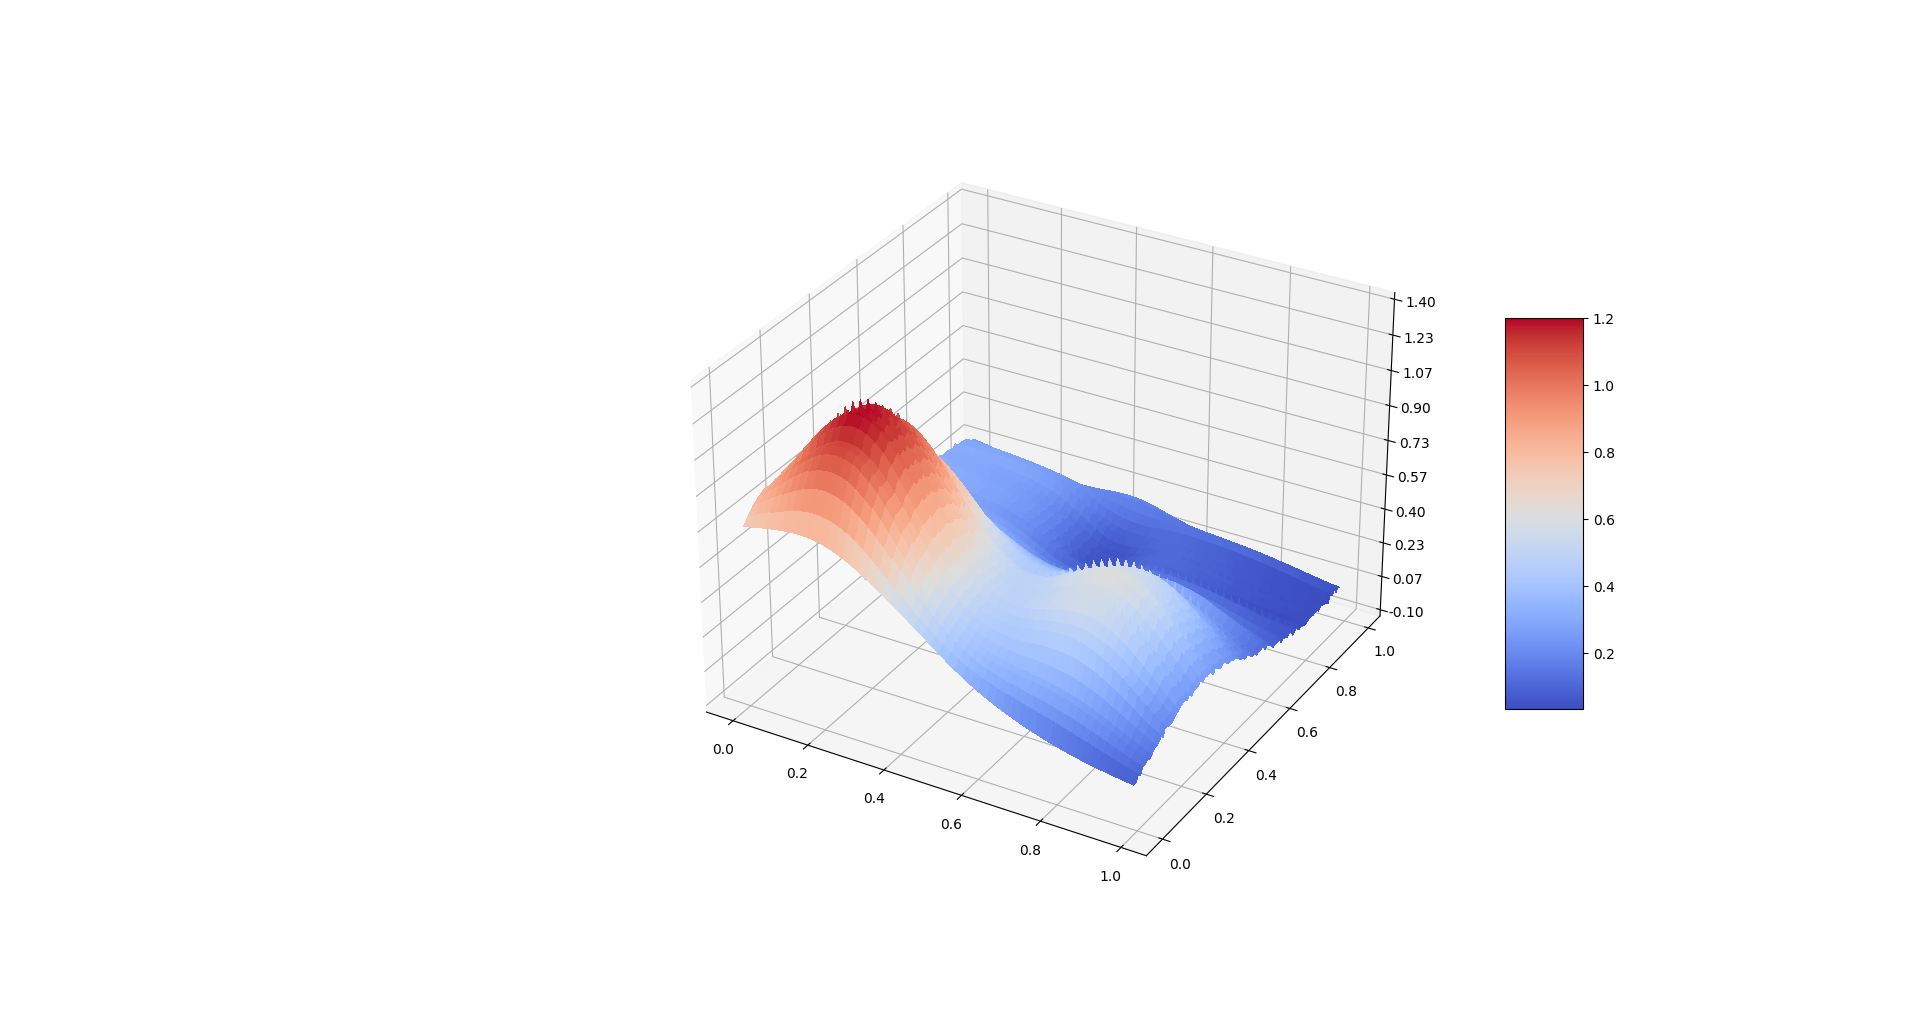
\includegraphics[width = 1\linewidth]{C:/Users/Sander/Documents/GitHub/FYS-STK4155/Project1/Report/Figures/zEst_n100_p5_noise0001_ts025.PNG}
\caption{\label{fig:FrankeEst2} The estimated Franke function when we have $100$ observations and polynomials of degree $5$ using a noise-level of $0.001$ and a $75/25$ train/test split.}
\end{figure}

\begin{figure}[H]
\centering
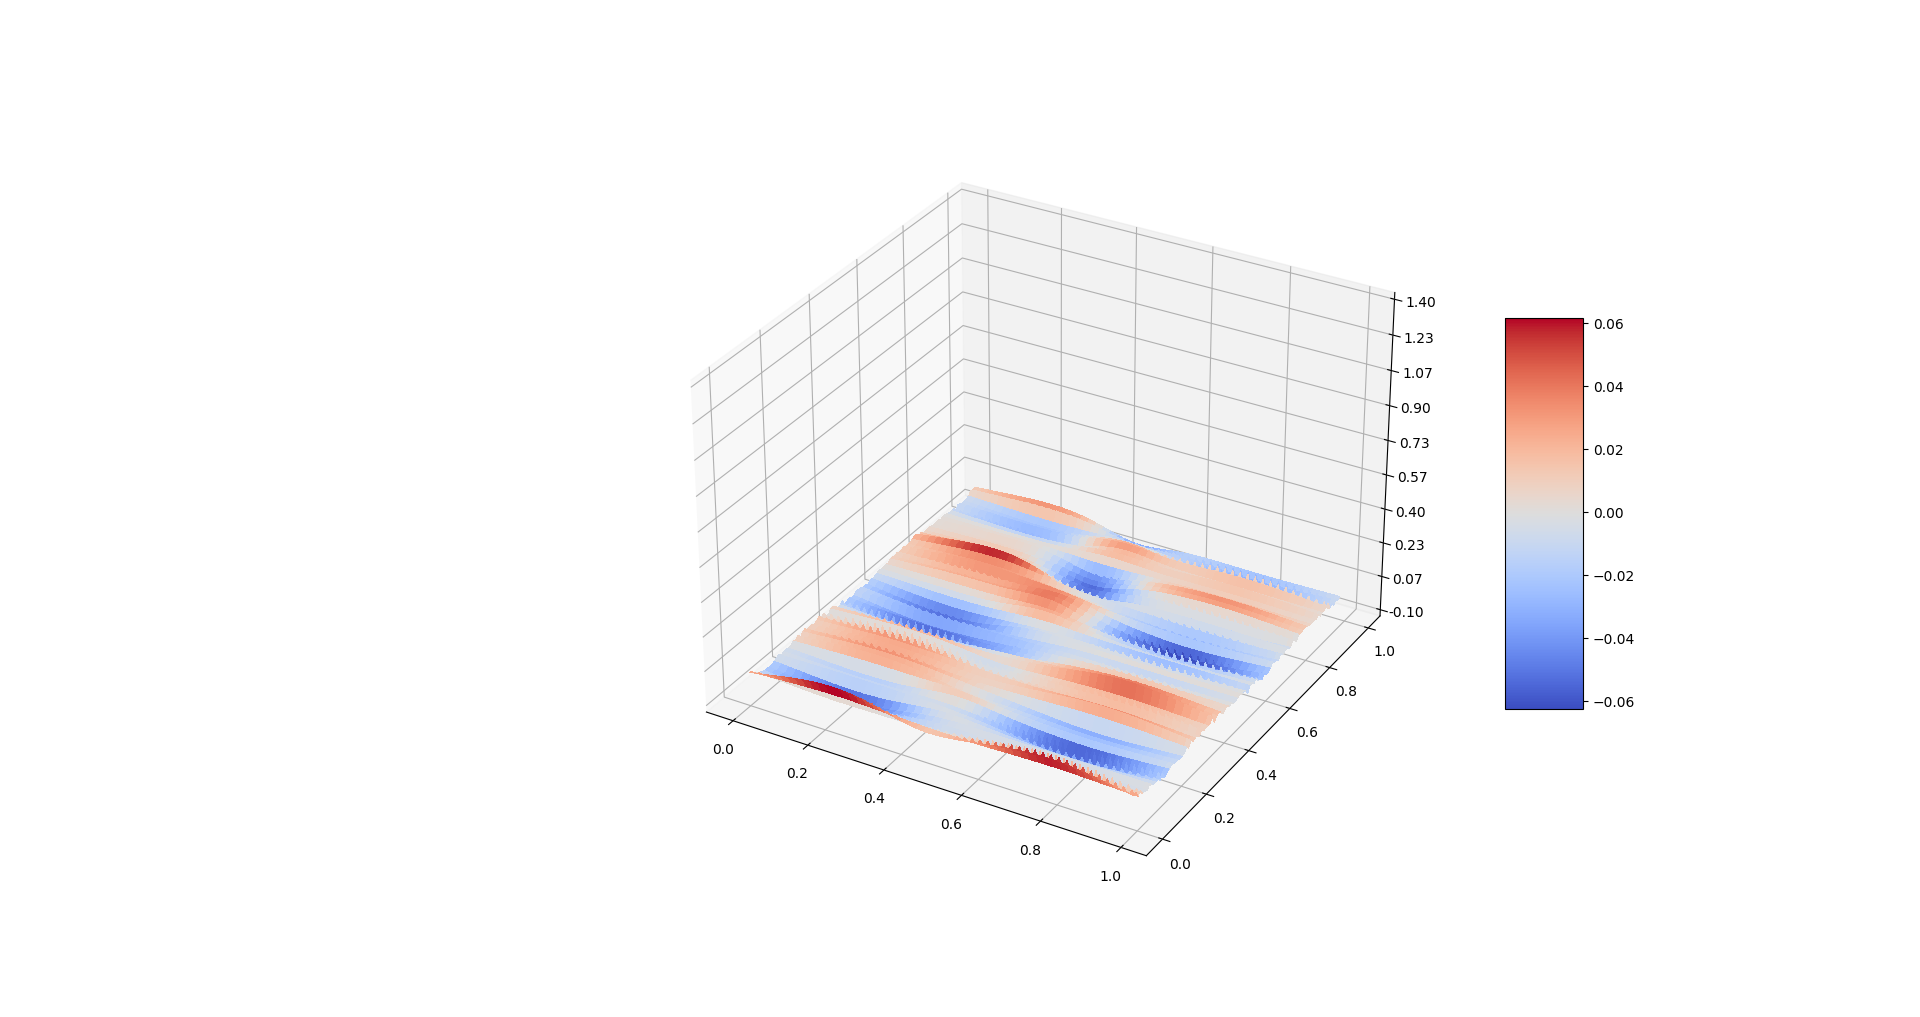
\includegraphics[width = 1\linewidth]{C:/Users/Sander/Documents/GitHub/FYS-STK4155/Project1/Report/Figures/zDiff_n100_p5_noise0001_ts025.PNG}
\caption{\label{fig:FrankeDIFF2} The difference between the real and estimated Franke functions when we have $100$ observations and polynomials of degree $5$ using a noise-level of $0.001$ and a $75/25$ train/test split.}
\end{figure}

\noindent We first observe that the figure is much smoother than the previous ones, as the function is discretized by n. We can again get a better understanding of these plots by finding the MSE and $R^2$ as shown in table \ref{tab:ESTREAL2}

\begin{table}[h]
\caption{\label{tab:ESTREAL2} MSE and $R^2$ between the real and estimated Franke function when we have $100$ observations and polynomials of degree $5$ using a noise-level of $0.001$ and a $75/25$ train/test split.}
\centering
\begin{tabular}{c|c|c}
 & MSE & $R^2$\\
\hline
Training & $0.006495$ & $0.920514$\\
\hline
Test & $0.028460$ & $0.660724$\\	  
\end{tabular}
\end{table}

\noindent One can observe from table \ref{tab:ESTREAL2} that the test MSE is much lower with $n = 100$ than with $n = 10$ and also the $R^2$ is higher. Therefore it is safe to say that increasing the number of observations drastically increases the predictive capability of the model. The training MSE and $R^2$ is not really of any importance, as we simply want the model to be able to predict future data. 
\\
Furthermore, we can compare figure \ref{fig:betaIntALL2} and figure \ref{fig:betaIntALL1} to see that the confidence of our regression coefficients increase as we increase n. This is actually the reason why the model improves.

\begin{figure}[H]
\centering
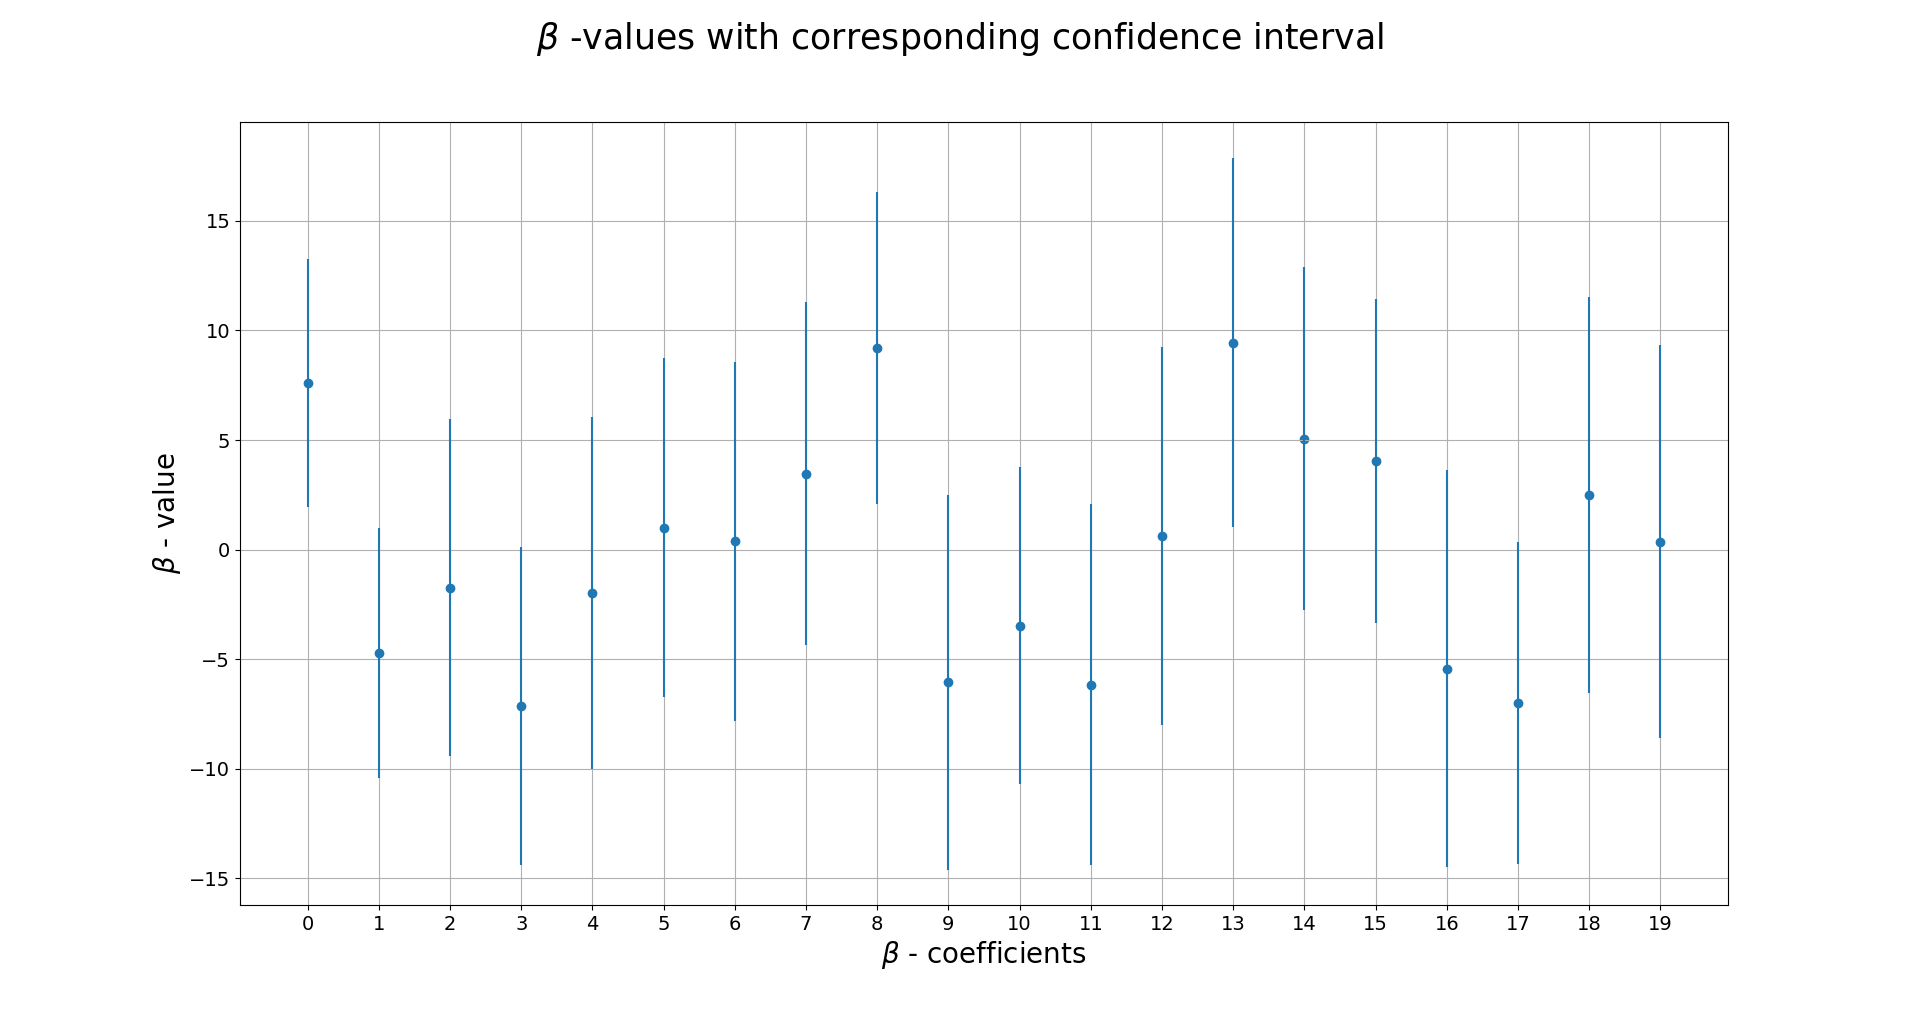
\includegraphics[width = 1\linewidth]{C:/Users/Sander/Documents/GitHub/FYS-STK4155/Project1/Report/Figures/tablllll.PNG}
\caption{\label{fig:betaIntALL2} $\hat{\boldsymbol{\beta}}$-coefficients from performing ordinary least squares regression. Dots indicate the actual $\hat{\boldsymbol{\beta}}$-coefficients value while bars around indicate the confidence interval ($\pm \sigma$).}
\end{figure}

\noindent We can also see what happen if we were to increase the noise-level from $0.001$ to $0.1$ using $n = 100$ observations in figures \ref{fig:FrankeEst3}

\begin{figure}[h]
\centering
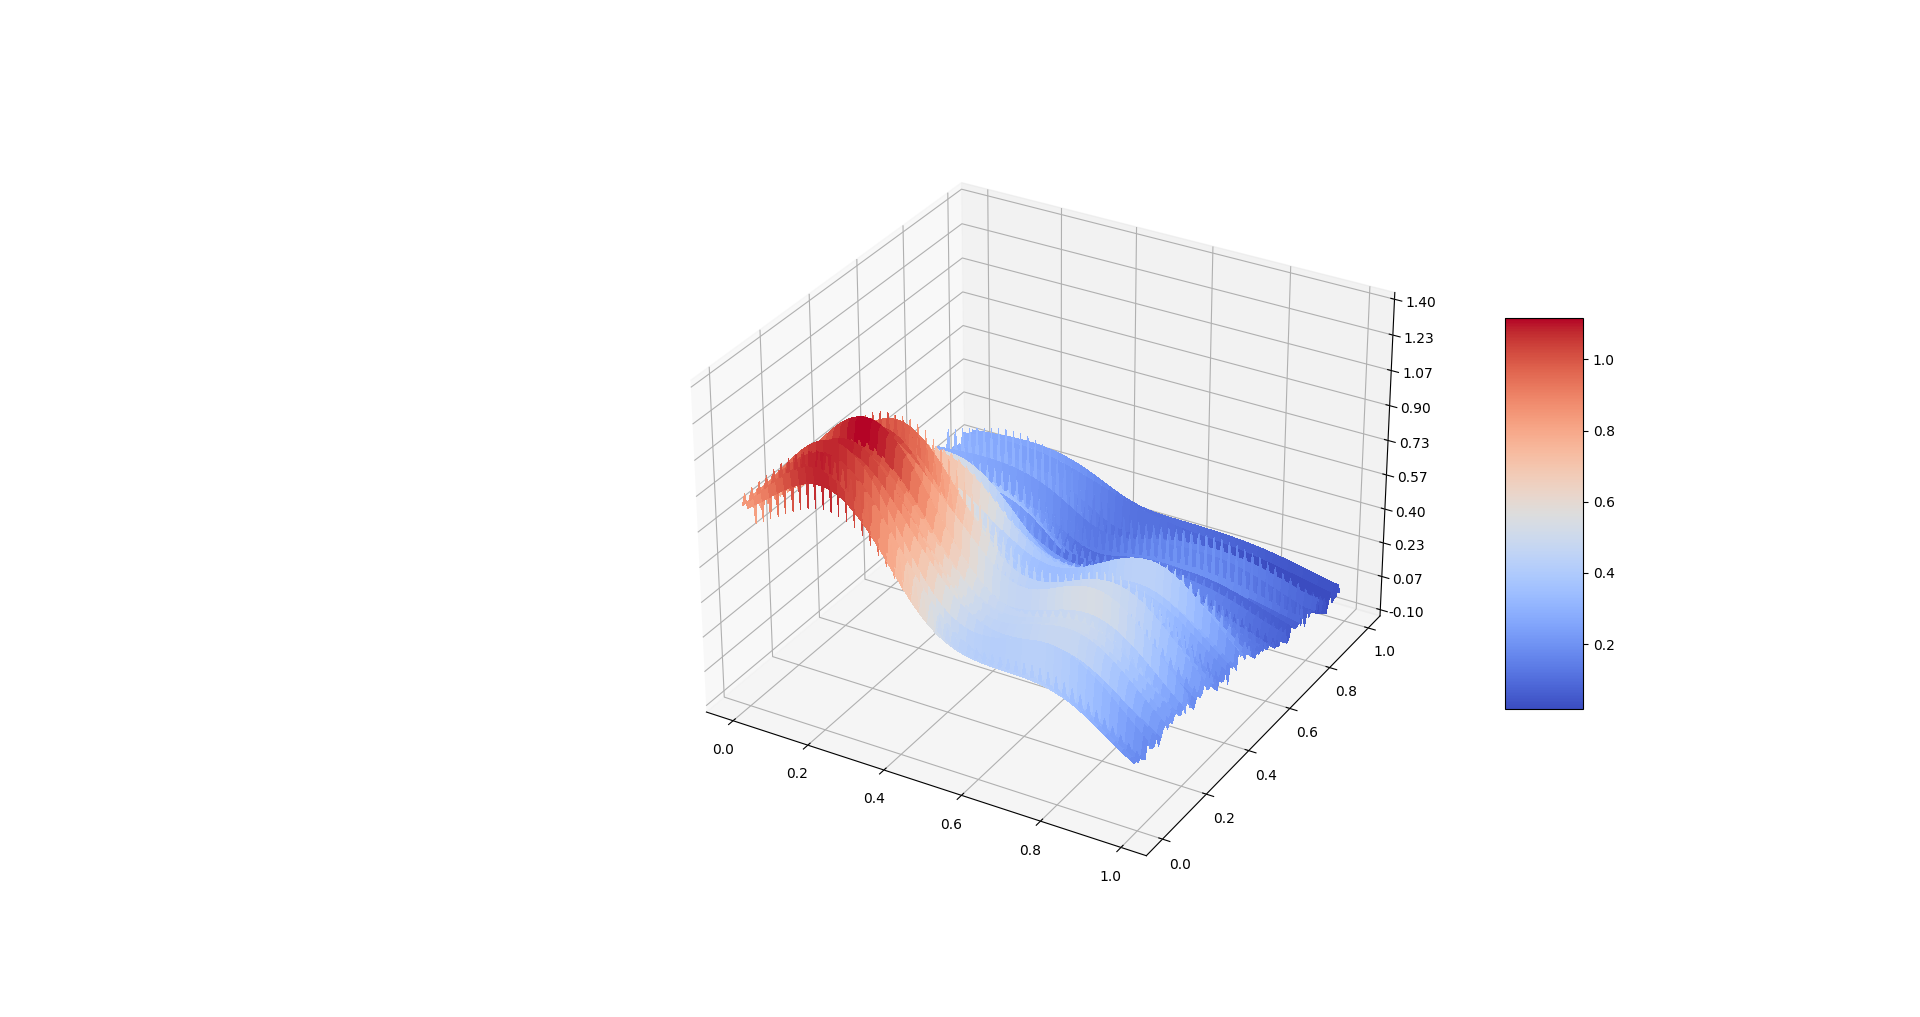
\includegraphics[width = 1\linewidth]{C:/Users/Sander/Documents/GitHub/FYS-STK4155/Project1/Report/Figures/zEst_n100_p5_noise01_ts025.PNG}
\caption{\label{fig:FrankeEst3} The estimated Franke function when we have $100$ observations and polynomials of degree $5$ using a noise-level of $0.1$ and a $75/25$ train/test split.}
\end{figure}

\noindent As expected, the noise makes the model worse at predicting $\hat{y}$. However, the overall traits of the Franke function can still be observed, but the errors shown in table \ref{tab:ESTREAL3} indicates that the performance is worse with more noise

\begin{table}[H]
\caption{\label{tab:ESTREAL3} MSE and $R^2$ between the real and estimated Franke function when we have $100$ observations and polynomials of degree $5$ using a noise-level of $0.1$ and a $75/25$ train/test split.}
\centering
\begin{tabular}{c|c|c}
 & MSE & $R^2$\\
\hline
Training & $0.07546367560674669$ & $0.023928247975465555$\\
\hline
Test & $0.15827698280851488$ & $0.01920380609030712$\\	  
\end{tabular}
\end{table}

\noindent We could easily remove all the noise from the model, but we intend to keep a noise level of $0.001$ as it will prepare us for the real data later in the project. Furthermore, we now look at the MSE at different values of complexity p. Table \ref{tab:asp} shows test and train MSE for different values of p

\begin{table}[H]
\caption{\label{tab:asp} Different values of train/test MSE/$R^2$ using 100 observations, a noise-level of $0.001$, scaled data and a $75/25$ train test split.}
\centering
\begin{tabular}{c|c|c|c|c}
 & Train MSE & Test MSE & Train $R^2$ & Test $R^2$\\
\hline
$p = 3$ & $0.024277$ & $0.063425$ & $0.709721$ & $0.193302$\\
\hline
$p = 4$ & $0.010872$ & $0.016600$ & $0.875196$ & $0.757525$\\
\hline
$p = 5$ & $0.006495$ & $0.028460$ & $0.920514$ & $0.660724$\\
\hline
$p = 6$ & $0.007942$ & $0.029148$ & $0.904951$ & $0.629532$\\
\hline
$p = 7$ & $0.006291$ & $0.027968$ & $0.924537$ & $0.649141$\\
\hline
$p = 30$ & $1.435312e-22$ & $0.041373$ & $1.0$ & $0.504594$\\
\end{tabular}
\end{table}

\noindent One can observe that the train MSE keeps decreasing with model complexity, while the test MSE decreases to some point and then starts to increase. The inverse is true for the $R^2$s. How to find the point of minimum MSE will be the topic of the next exercise.


\newpage

\begin{center}
\Large{\textbf{Exercise 1b): Mean square error as function of model complexity and bootstrap resampling.}}
\end{center}

\begin{center}
\large{\textbf{MSE decomposition}}
\end{center}

\noindent When we fit a linear model like in the last exercise, we always want to minimize the MSE of the test set. We can explain the MSE from equation \ref{eq:MSE} in terms of the expected value instead of the mean. This assumption only holds when n is large, but let's assume that it is. Then the MSE is simply the expected value of the difference between the actual response and the predicted response using regression. This mean we can write the MSE as $E[(y-\hat{y})^2]$ where y is the actual response while $\hat{y}$ is the predicted response. By adding and subtracting the term $E[\hat{y}]$ to the inner bracket we can expand the MSE like in equation \ref{eq:mseDerive}

\begin{equation}\label{eq:mseDerive}
\begin{aligned}
MSE = E[(y-\hat{y})^2] = E[(y-\hat{y} + E[\hat{y}] - E[\hat{y}])^2]
\\
E[(\hat{y} - E[\hat{y}])^2 + 2(\hat{y} - E[\hat{y}])(E[\hat{y}]-y) + (E[\hat{y}]-y)^2]
\\
E[(\hat{y} - E[\hat{y}])^2] + E[2(\hat{y} - E[\hat{y}])(E[\hat{y}]-y)] + E[(E[\hat{y}]-y)^2]
\end{aligned}
\end{equation}

\noindent Since the expected value of $\hat{y}$ equals y when n is large, we can write $E[\hat{y}] - y =$ constant and thus

\begin{equation}\label{eq:mseDerive2}
\begin{aligned}
E[(\hat{y} - E[\hat{y}])^2] + 2(E[\hat{y}]-y)E[\hat{y}-E[\hat{y}]] + (E[\hat{y}]-y)^2
\\
E[(\hat{y} - E[\hat{y}])^2] + 2(E[\hat{y}]-y)(E[\hat{y}] - E[\hat{y}])+ (E[\hat{y}]-y)^2
\\
E[(\hat{y} - E[\hat{y}])^2] + (E[\hat{y}]-y)^2
\end{aligned}
\end{equation}

\noindent where the constant $E[\hat{y}] - E[\hat{y}]$ equals zero, making the whole term equal zero. 
\\
We recognize the term $E[(\hat{y} - E[\hat{y}])^2]$ as the variance of the estimator $\hat{y}$ and the term $(E[\hat{y}]-y)^2$ as the bias of the model, but squared. The bias quantifies how well the model fits the data points and variance is how well the model would translate to other data the model is not trained on. Increasing one tends to decrease the other, but not linearly since the bias is squared. Therefore, one can decrease the bias to a certain extent, but at some point, the loss of bias is not worth the gain in variance. This is called the bias variance trade-off. 

\begin{center}
\large{\textbf{Bootstrapping}}
\end{center}

\noindent Before investigating the bias-variance trade-off any further, we need to solve a problem related to the lack of data that is often the case with real data. When we generate data synthetically, the lack of data is never a problem, but in the real world, data is always limited and we now want to simulate that experience. Imagine now that we only have 100 observations and that these 100 observations are enough to represent the underlying distribution of the data, but not enough for our machine learning algorithm to function properly. We can then utilize the bootstrap resampling method to "create data out of thin air". The bootstrap resampling method aims to take the original data of size n and create B new data sets each of size n. This is done by randomly assigning observations from the original data set to the B new data sets (with replacement). Then, a statistic is calculated for each of the B new data sets and the mean of all these statistics should represent the statistic of the original data set (James, G., et al., 2017, [A]). The new statistic is often called the bootstrap statistic and will in this report be the MSE. Figure \ref{fig:Bootsketch} shows a rough sketch of the process

\begin{figure}[H]
\centering
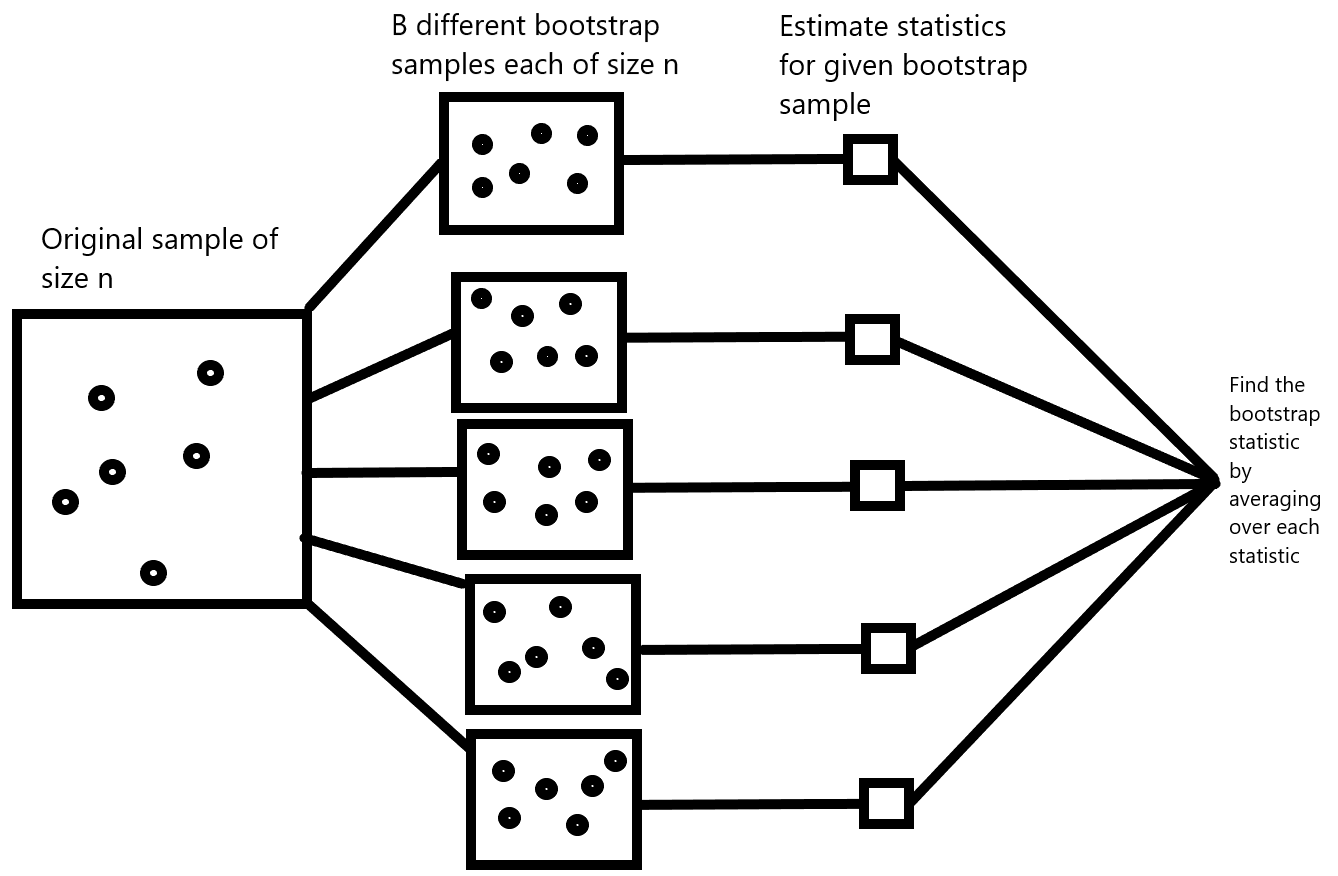
\includegraphics[width = 1\linewidth]{C:/Users/Sander/Documents/GitHub/FYS-STK4155/Project1/Report/Figures/bootstrapSketch.PNG}
\caption{\label{fig:Bootsketch} Illustration of the bootstrap process. The statistic in question here is the MSE.}
\end{figure}

\noindent The hope of the bootstrap method is that the bootstrap statistic represents the statistic of the underlying distribution of the original data set, regardless of the original datasets distribution. Be aware, the bootstrap method does not create new information, but simply exaggerate the already existing information, letting us perform operations like linear regression more easily.

\begin{center}
\large{\textbf{MSE as function of model complexity}}
\end{center}

\noindent Now that we have a method of creating more data, we can study the bias-variance trade-off more thoroughly. More spesifically, we want to study how the bias, variance and MSE changes as a function of polynomial degree. Now imagine we just have 100 observations. We can then utilize the bootstrap resampling method to create $B \times n$ more data. Let us generate $B = 100$ data sets each of size n and see how the MSE changes as function of polynomial degree as seen in figures \ref{fig:MSEBOOT1} and \ref{fig:BVBOOT1}

\begin{figure}[H]
\centering
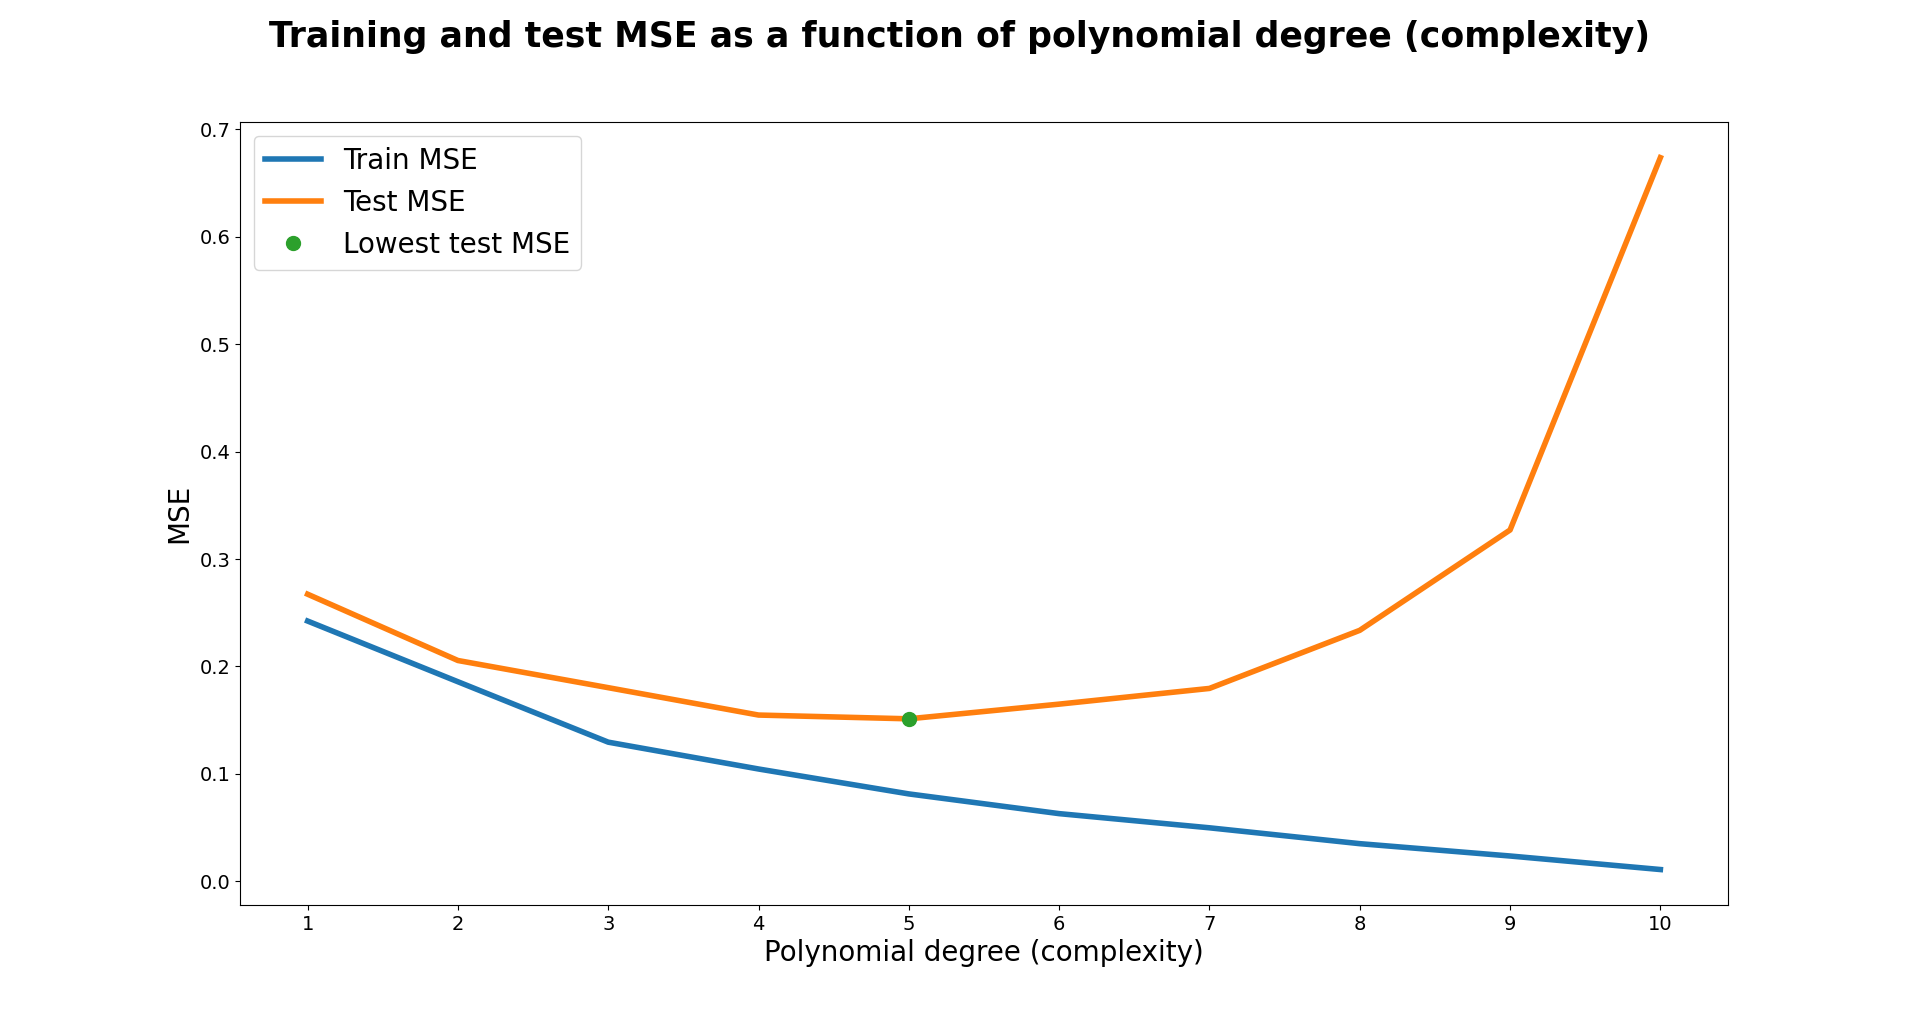
\includegraphics[width = 1\linewidth]{C:/Users/Sander/Documents/GitHub/FYS-STK4155/Project1/Report/Figures/MSEBOOT_n1000_p10_noise0001_ts025_B100_shuffles.PNG}
\caption{\label{fig:MSEBOOT1} MSE as a function of polynomial degree using the bootstrap resampling method. Here we have 100 observations while we generate 100 bootstrap samples with a noise level of $0.001$ and a $75/25$ train test split.}
\end{figure}

\begin{figure}[H]
\centering
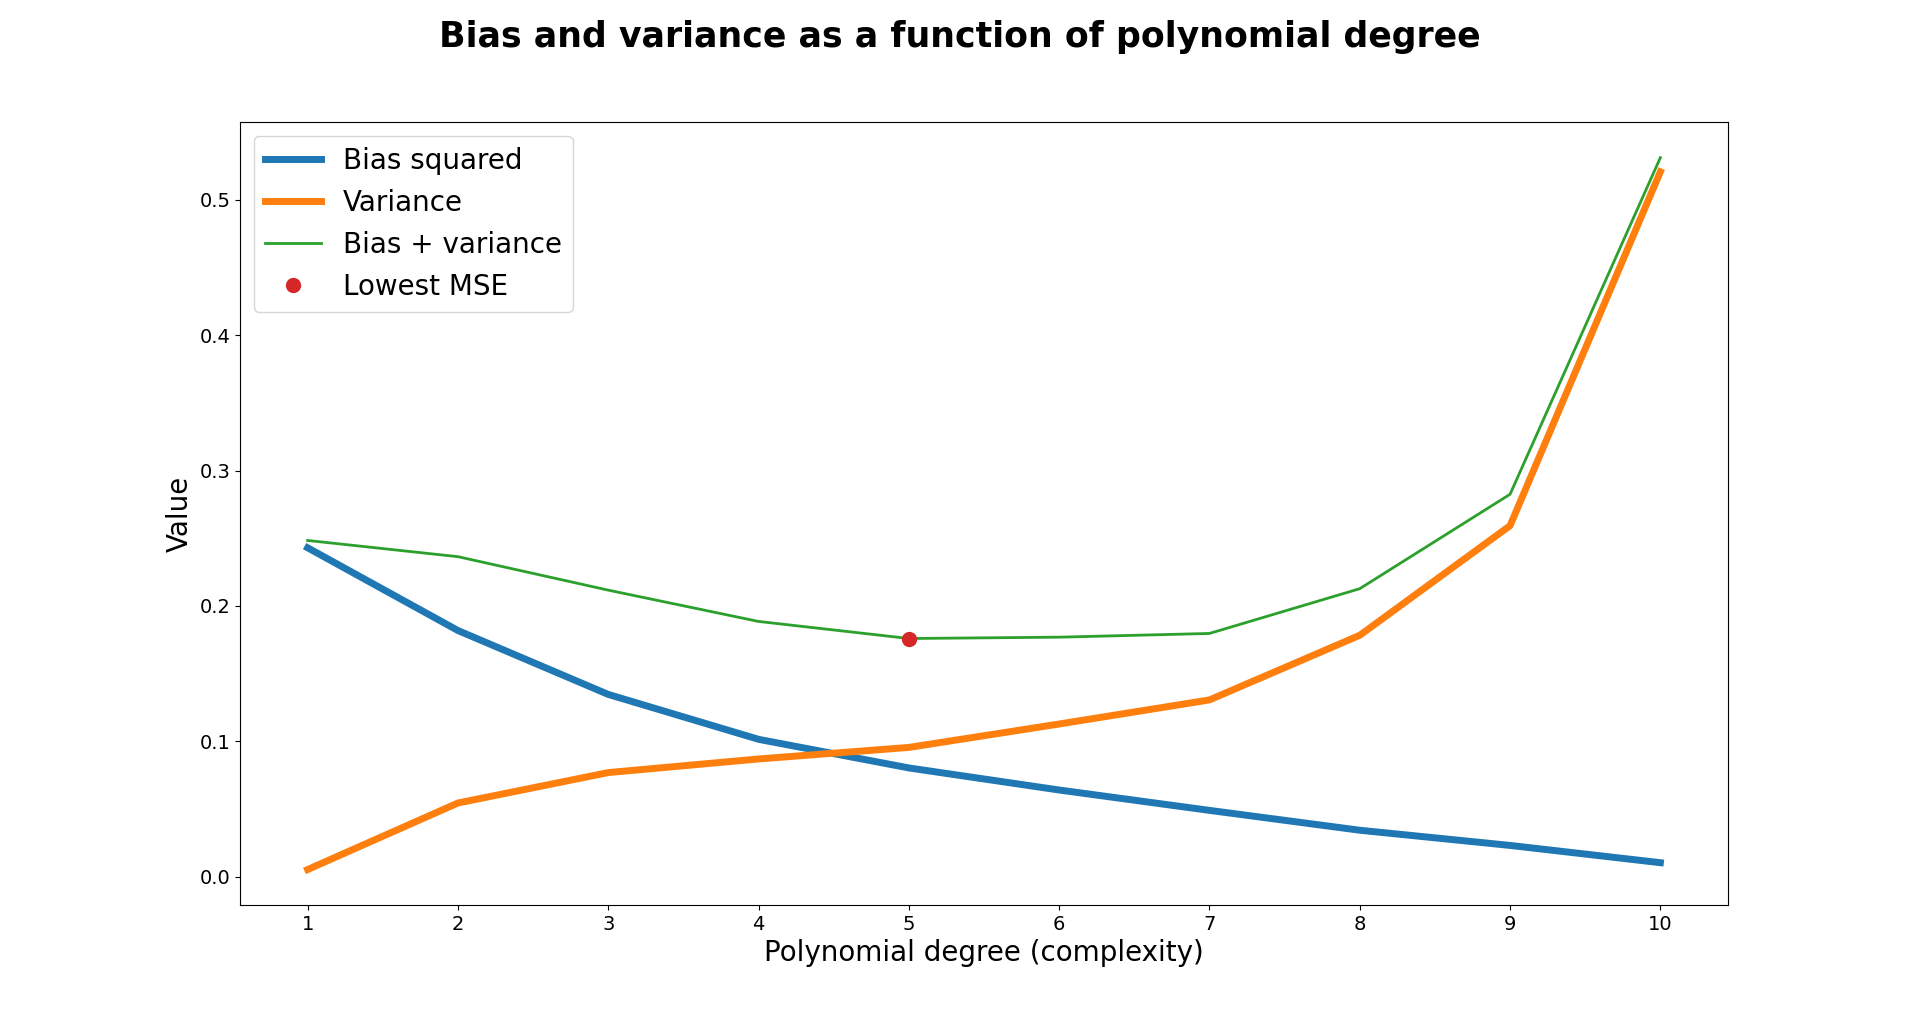
\includegraphics[width = 1\linewidth]{C:/Users/Sander/Documents/GitHub/FYS-STK4155/Project1/Report/Figures/BVplotBOOT_n1000_p10_noise0001_ts025_B100_shuffles.PNG}
\caption{\label{fig:BVBOOT1} Bias and variance decomposition of figure \ref{fig:MSEBOOT1}. The bias and variance change as a function of polynomial degree using the bootstrap resampling method. Here we have 100 observations while we generate 100 bootstrap samples with a noise level of $0.001$ and a $75/25$ train test split.}
\end{figure}

\noindent We can observe that the bias starts high, but tends towards zero when we increase the complexity of our model. This is because a low order polynomial is unable to fit data data points of the complex Franke function to a sufficient degree, thus making the distance between the model and the actual Franke function large, leading to higher MSE. When the polynomials degree gets larger however, the model can be fit arbitrarily close to the actual Franke function. 
\\
The variance behaves almost the opposite of the bias as it starts very low, but increases along with the complexity. This is because a low order polynomial would manage to somewhat fit both the training and test set equally bad. When we increase the complexity, the model fits the training data very well, but is unable to accurately predict the test data as the trained model is too complex, leading to over-fitting. 
\\
We can also see that the minimum MSE in figure \ref{fig:MSEBOOT1} corresponds to the same polynomial as that of figure \ref{fig:BVBOOT1}, strengthening our trust in the models predictive capabilities, but what would happen if we were to decrease the number of bootstrap samples? Let us now generate a new model where all the parameters are the same as of the previous one, but where we only generate 10 bootstrap samples. Then we get something akin to figure \ref{fig:MSEBOOT2}

\begin{figure}[H]
\centering
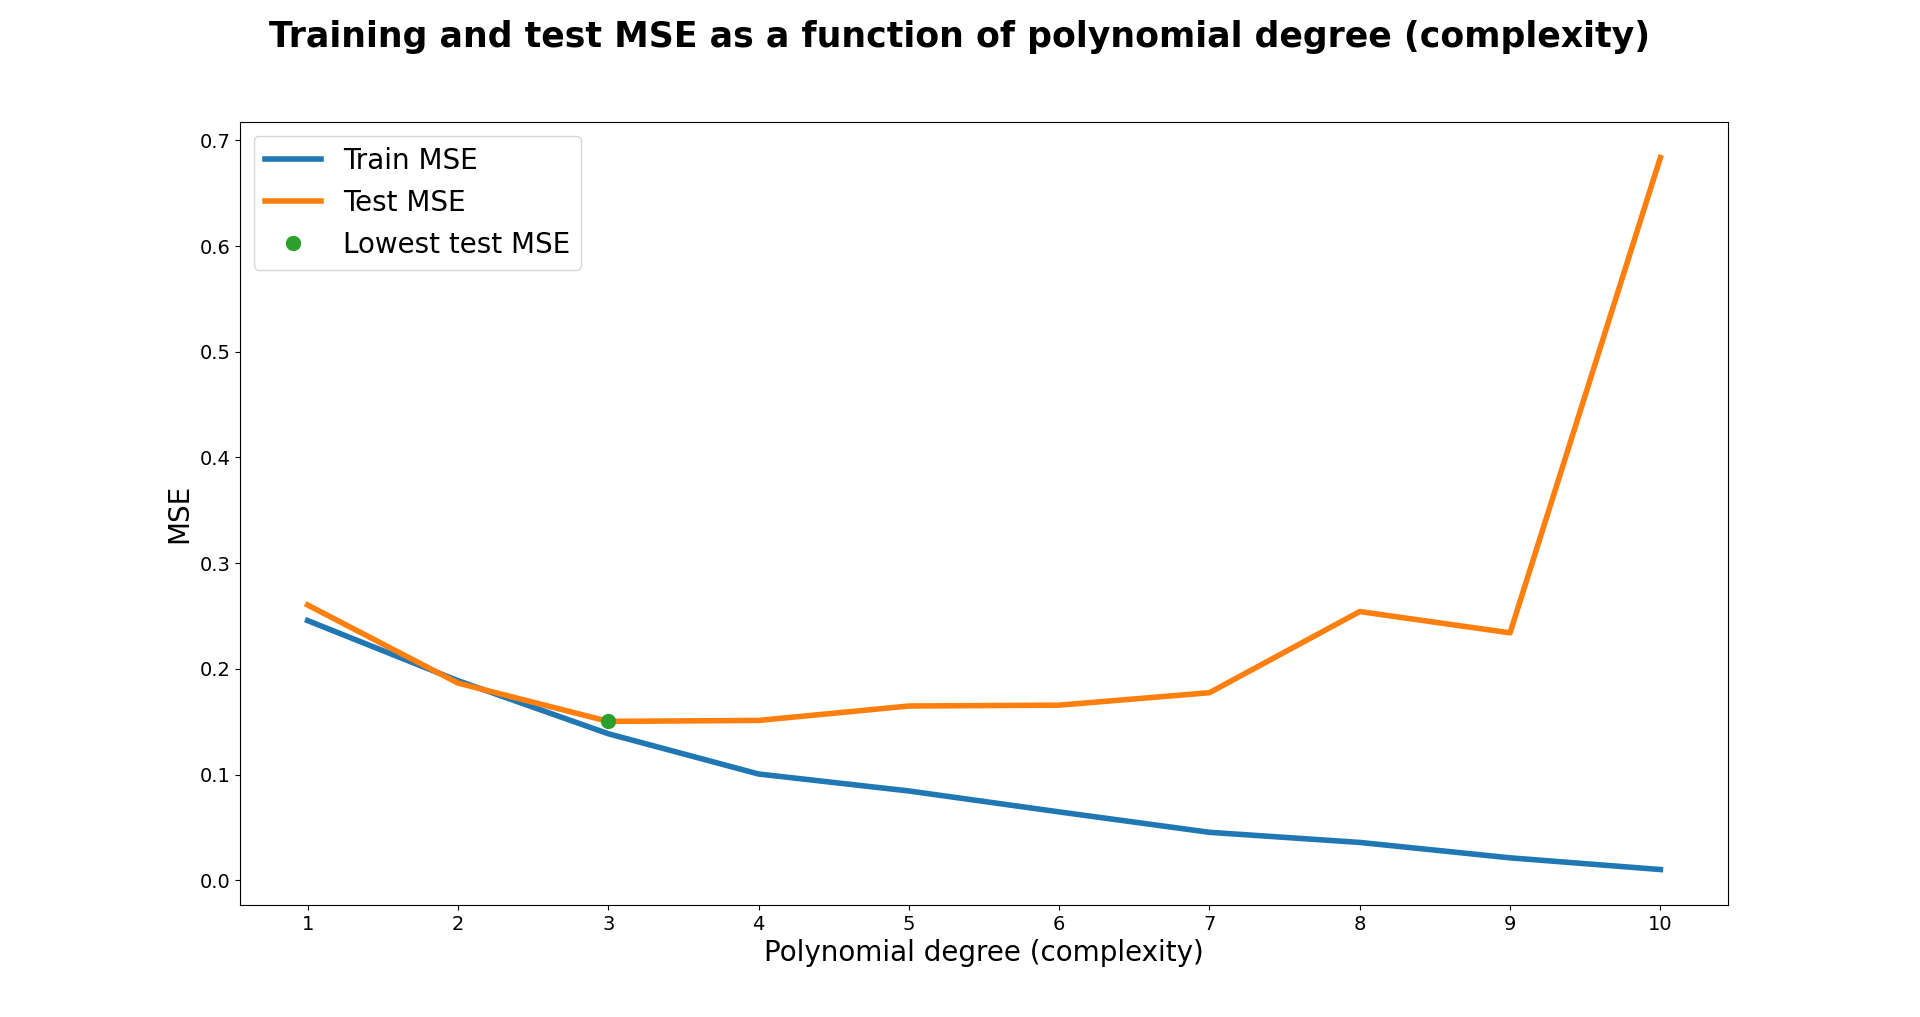
\includegraphics[width = 1\linewidth]{C:/Users/Sander/Documents/GitHub/FYS-STK4155/Project1/Report/Figures/MSEBOOT_n1000_p10_noise0001_ts025_B10_shuffles.PNG}
\caption{\label{fig:MSEBOOT2} MSE as a function of polynomial degree using the bootstrap resampling method. Here we have 100 observations while we generate 10 bootstrap samples with a noise level of $0.001$ and a $75/25$ train test split.}
\end{figure}

\noindent We can observe from figure \ref{fig:MSEBOOT2} that the point of lowest MSE is now at $p = 3$ which is lower than the one observed in figure \ref{fig:MSEBOOT1}. This is because more data means that the model can be trained more without over-fitting (Vittinghoff, E., et al., 2005). Thus, when we decrease the number of observations (or bootstrap samples in this case), we lower the threshold for when the model becomes overfit. This again means that a lower degree of polynomial is the ideal complexity for the model. 
\\
What is also observed from the code when using a low amount of bootstrap samples is that the model becomes increasingly unstable. This is because the bootstrap MSE relies on the mean of the B generated statistics. If we only generate a few bootstrap samples, the mean is more prone to randomness, which in turn means the algorithm is unstable. For this reason and the one described above (more data is good), we want to stick with 100 bootstrap samples from here on out.

\newpage

\begin{center}
\large{\textbf{Exercise 1c): Mean square error as function of model complexity and cross-validation resampling.}}
\end{center}

\begin{center}
\large{\textbf{Cross-validation}}
\end{center}

\noindent We will now introduce another resampling method called cross-validation (CV) and repeat the analysis of the previous exercise. The cross-validation resampling method, like the bootstrap, also aims to "create more data out of thin air". However, the process is quite different than that of the bootstrap. The main idea behind the CV is to divide the original data set into k different data sets, or folds as they are called, and then let the kth fold act as the test set while the other k-1 folds acts as the training sets. Then the model is trained and a statistic (MSE) is calculated. Then, another fold will act as the test set while the others will act as the training set. This process repeats until every fold has been used as a test set once and a statistic for each permutation is calculated. The average of the k different statistic is then calculated and is said to represent the actual statistic of the original data set (James, G., et al., 2017, [B]). 
\\
It is typical to have 10, 5 or n folds and the CV process is then referred to as 10-fold, 5-fold and leave-one-out (LOOCV) cross-validation. The LOOCV is a special case of the CV method where each observations acts as the test set once and this process is sketched in figure \ref{fig:CVsketch}

\begin{figure}[H]
\centering
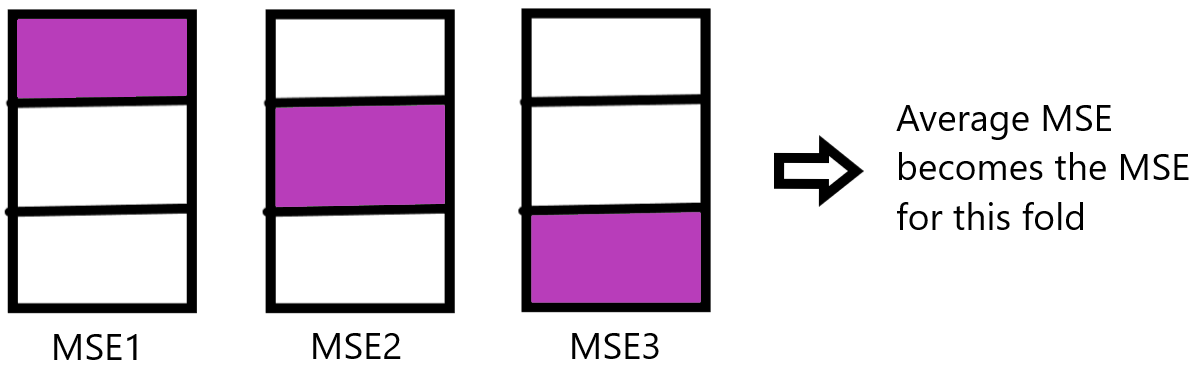
\includegraphics[width = 1\linewidth]{C:/Users/Sander/Documents/GitHub/FYS-STK4155/Project1/Report/Figures/CVSketch.PNG}
\caption{\label{fig:CVsketch} A rough sketch of the LOOCV process. The n observations acts as the test set once (purple squares) while the other $n-1$ observations acts as the training set (white squares). The model is then fit on each distinct permutation and a statistic is calculated (MSE in this project). Finally, an average of the k different statistics is calculated and will represent the statistic of the original data set.}
\end{figure}

\begin{center}
\large{\textbf{MSE as function of model complexity}}
\end{center}

\noindent We now want to repeat the process from the previous exercise where we see look at MSE as a function of polynomial degree for the 5-fold, 10-fold and leave one out cross-validations. Let us start with the 10-fold CV which is plotted in figure \ref{fig:MSECV1}

\begin{figure}[H]
\centering
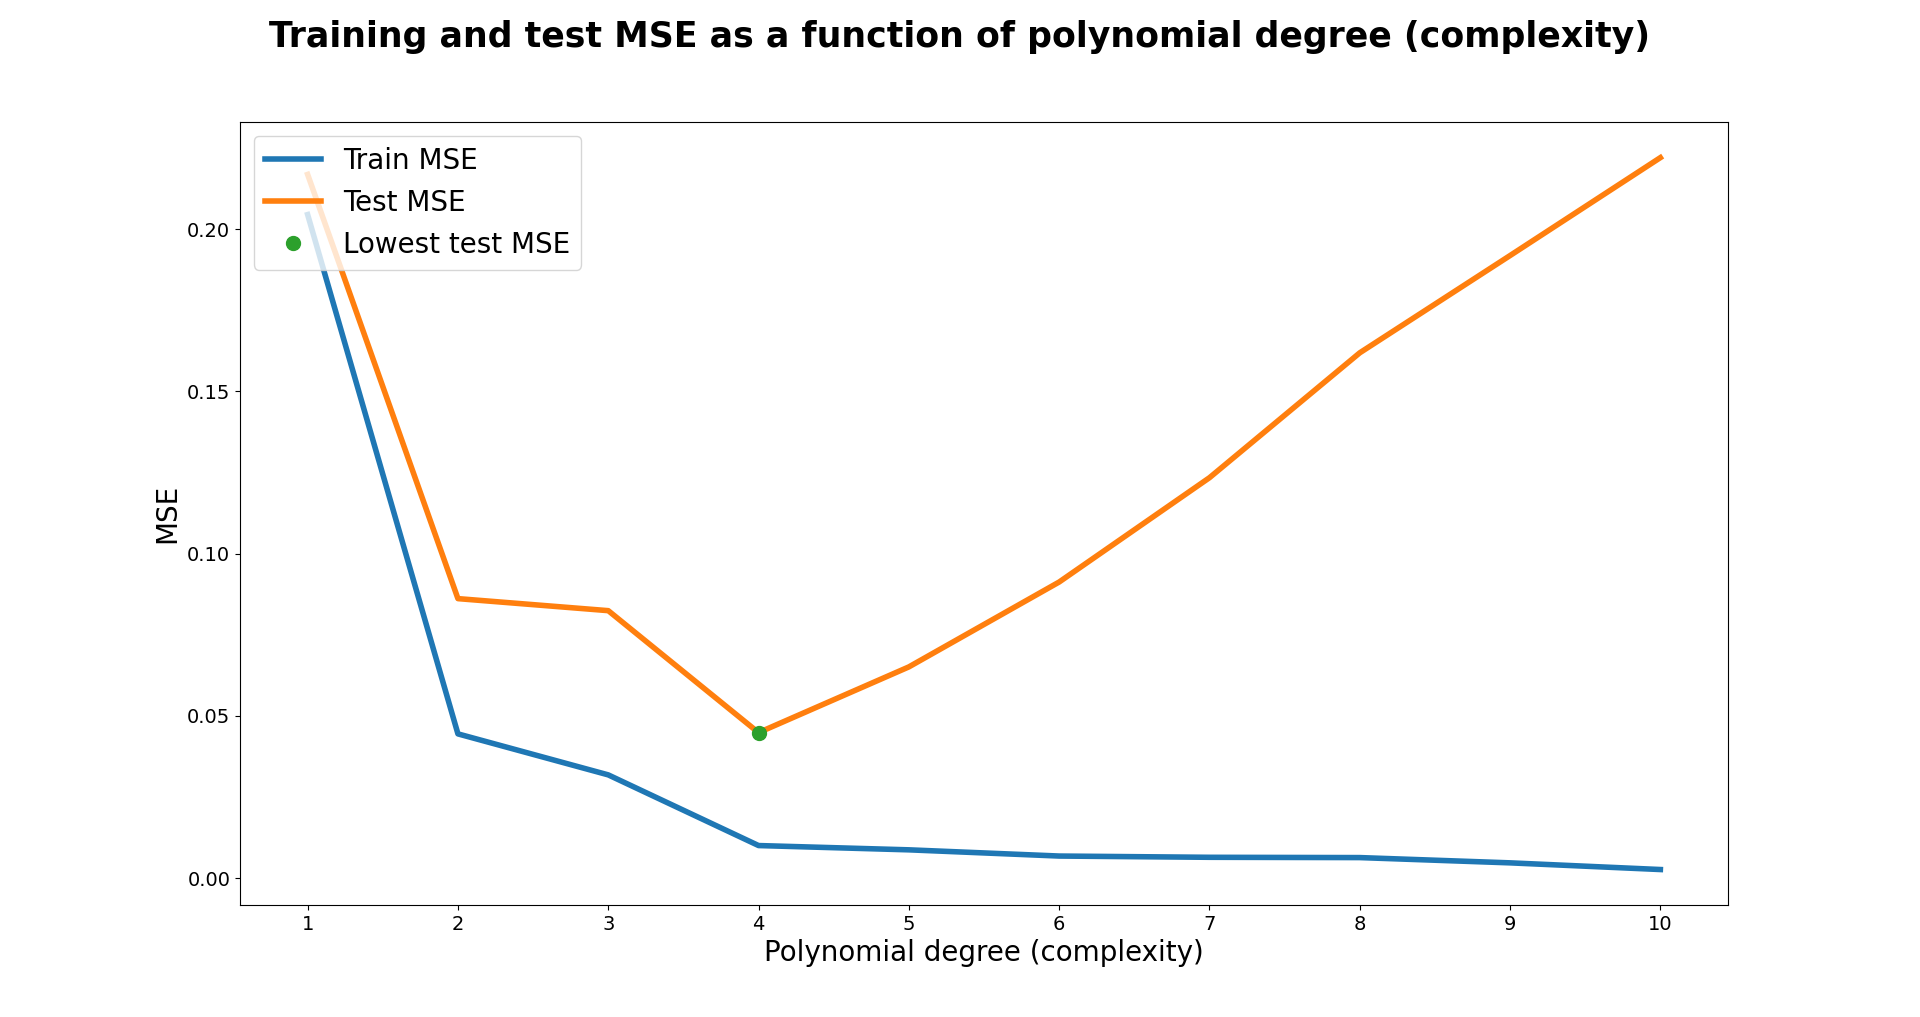
\includegraphics[width = 1\linewidth]{C:/Users/Sander/Documents/GitHub/FYS-STK4155/Project1/Report/Figures/MSECV_n100_p10_noise0001_CV10_shuffles.PNG}
\caption{\label{fig:MSECV1} MSE as a function of polynomial degree up to 10 using the 10-fold cross-validation resampling method. Here we have 100 observations while we split the data into 10 different folds with a noise level of $0.001$.}
\end{figure}

\noindent We can observe from figure \ref{fig:MSECV1} that the MSE is at its lowest for $p = 4$. We can decompose the MSE into its bias and variance components as done in figure \ref{fig:BVCV1}

\begin{figure}[H]
\centering
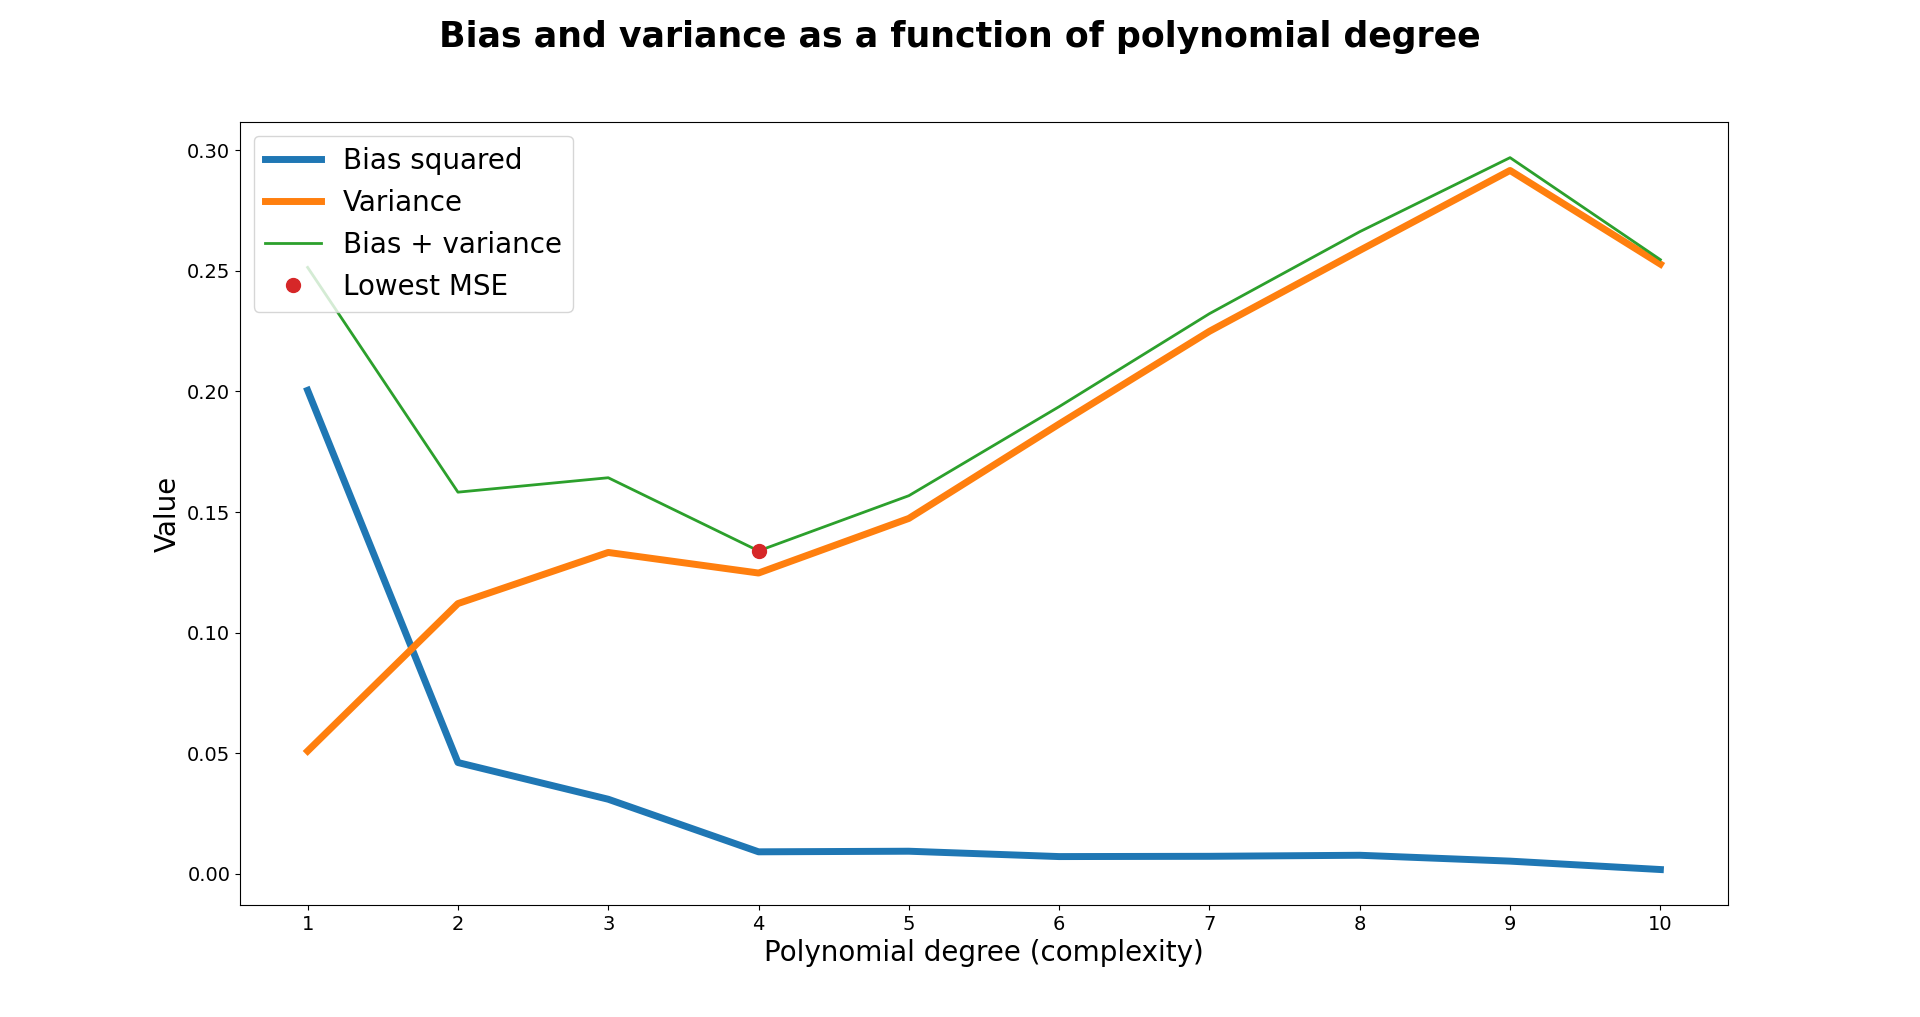
\includegraphics[width = 1\linewidth]{C:/Users/Sander/Documents/GitHub/FYS-STK4155/Project1/Report/Figures/BVplotCV_n100_p10_noise0001_CV10.PNG}
\caption{\label{fig:BVCV1} Bias and variance decomposition of figure \ref{fig:MSECV1}. Here we have 100 observations while we use 10-fold CV with a noise level of $0.001$.}
\end{figure}

\noindent It can be confirmed from figure \ref{fig:BVCV1} that the lowest MSE is found at $p = 4$ polynomial degrees. The bias and variance behaves similar to that of bootstrap as seen in figure \ref{fig:BVBOOT1}. 
\\
We now want to see what happens when we set the number of folds k equal to 5 and the result is shown in figures \ref{fig:MSECV2} and \ref{fig:BVCV2}

\begin{figure}[H]
\centering
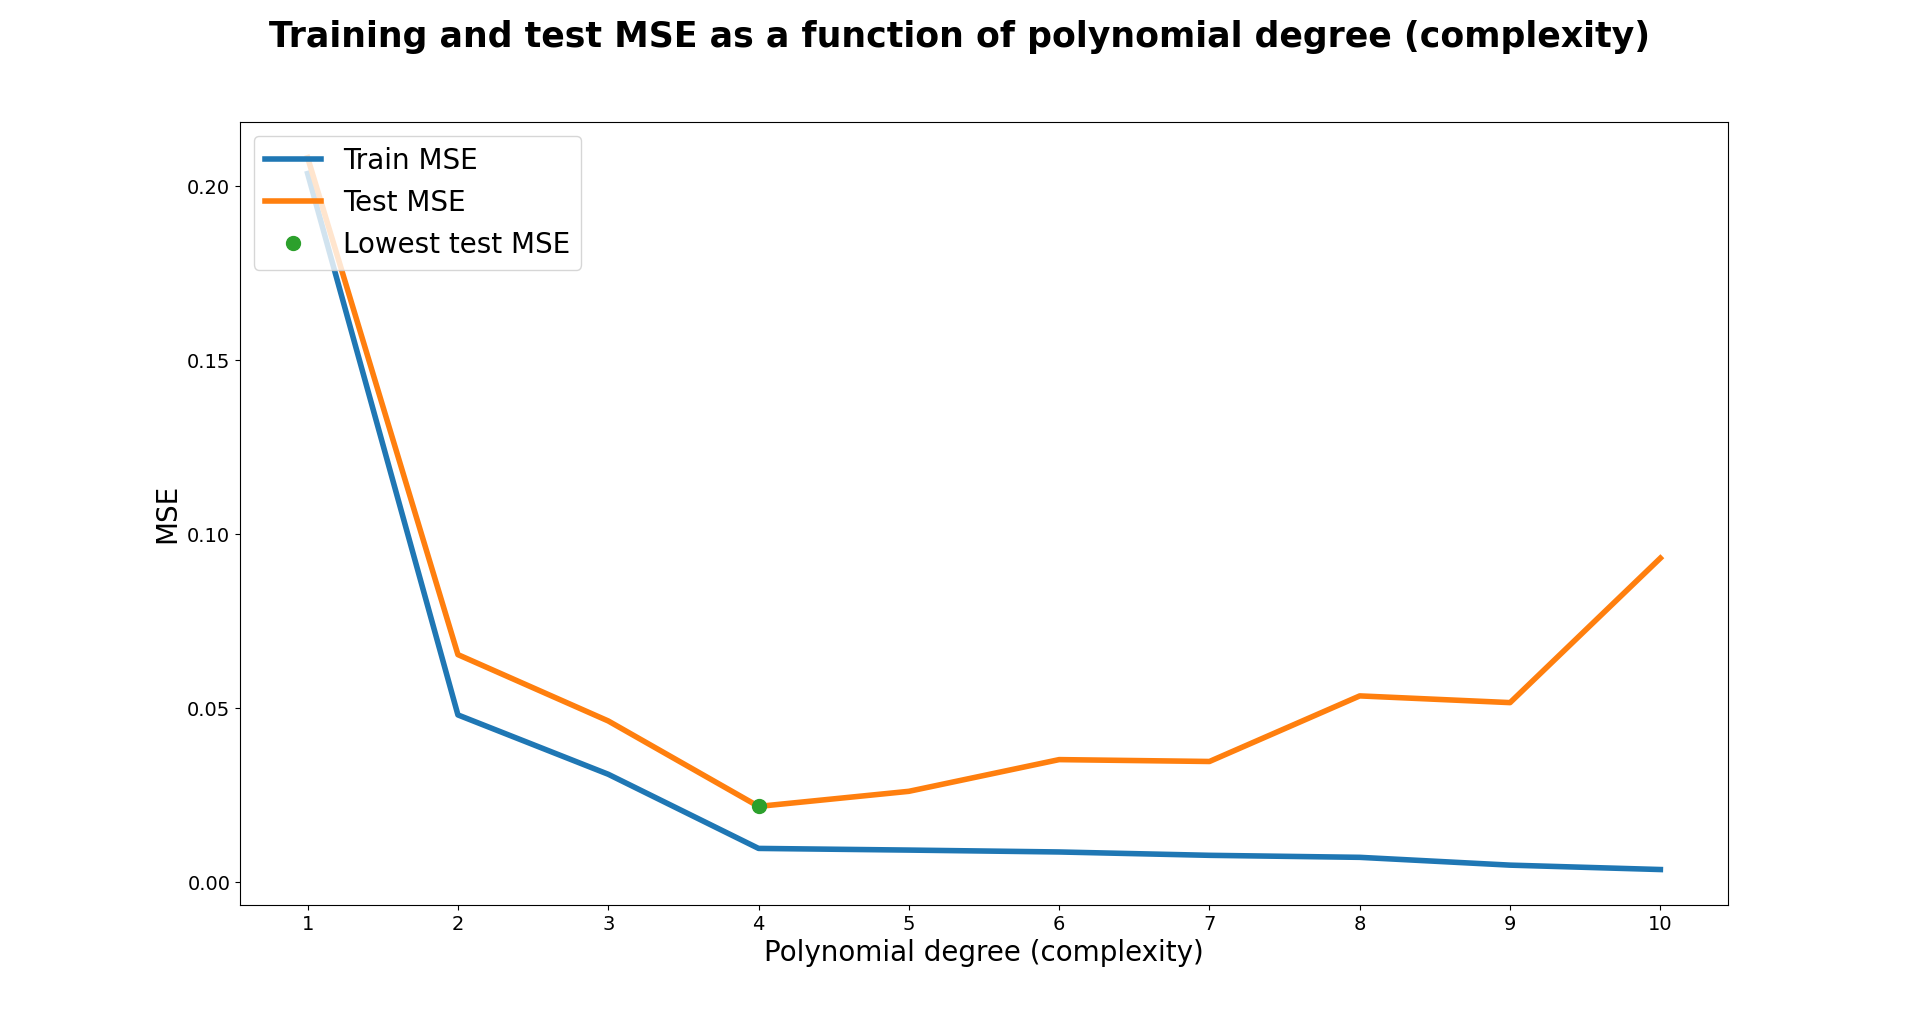
\includegraphics[width = 1\linewidth]{C:/Users/Sander/Documents/GitHub/FYS-STK4155/Project1/Report/Figures/MSECV_n100_p10_noise0001_CV5_shuffles.PNG}
\caption{\label{fig:MSECV2} MSE as a function of polynomial degree up to 10 using the 5-fold cross-validation resampling method. Here we have 100 observations while we split the data into 5 different folds with a noise level of $0.001$.}
\end{figure}

\begin{figure}[H]
\centering
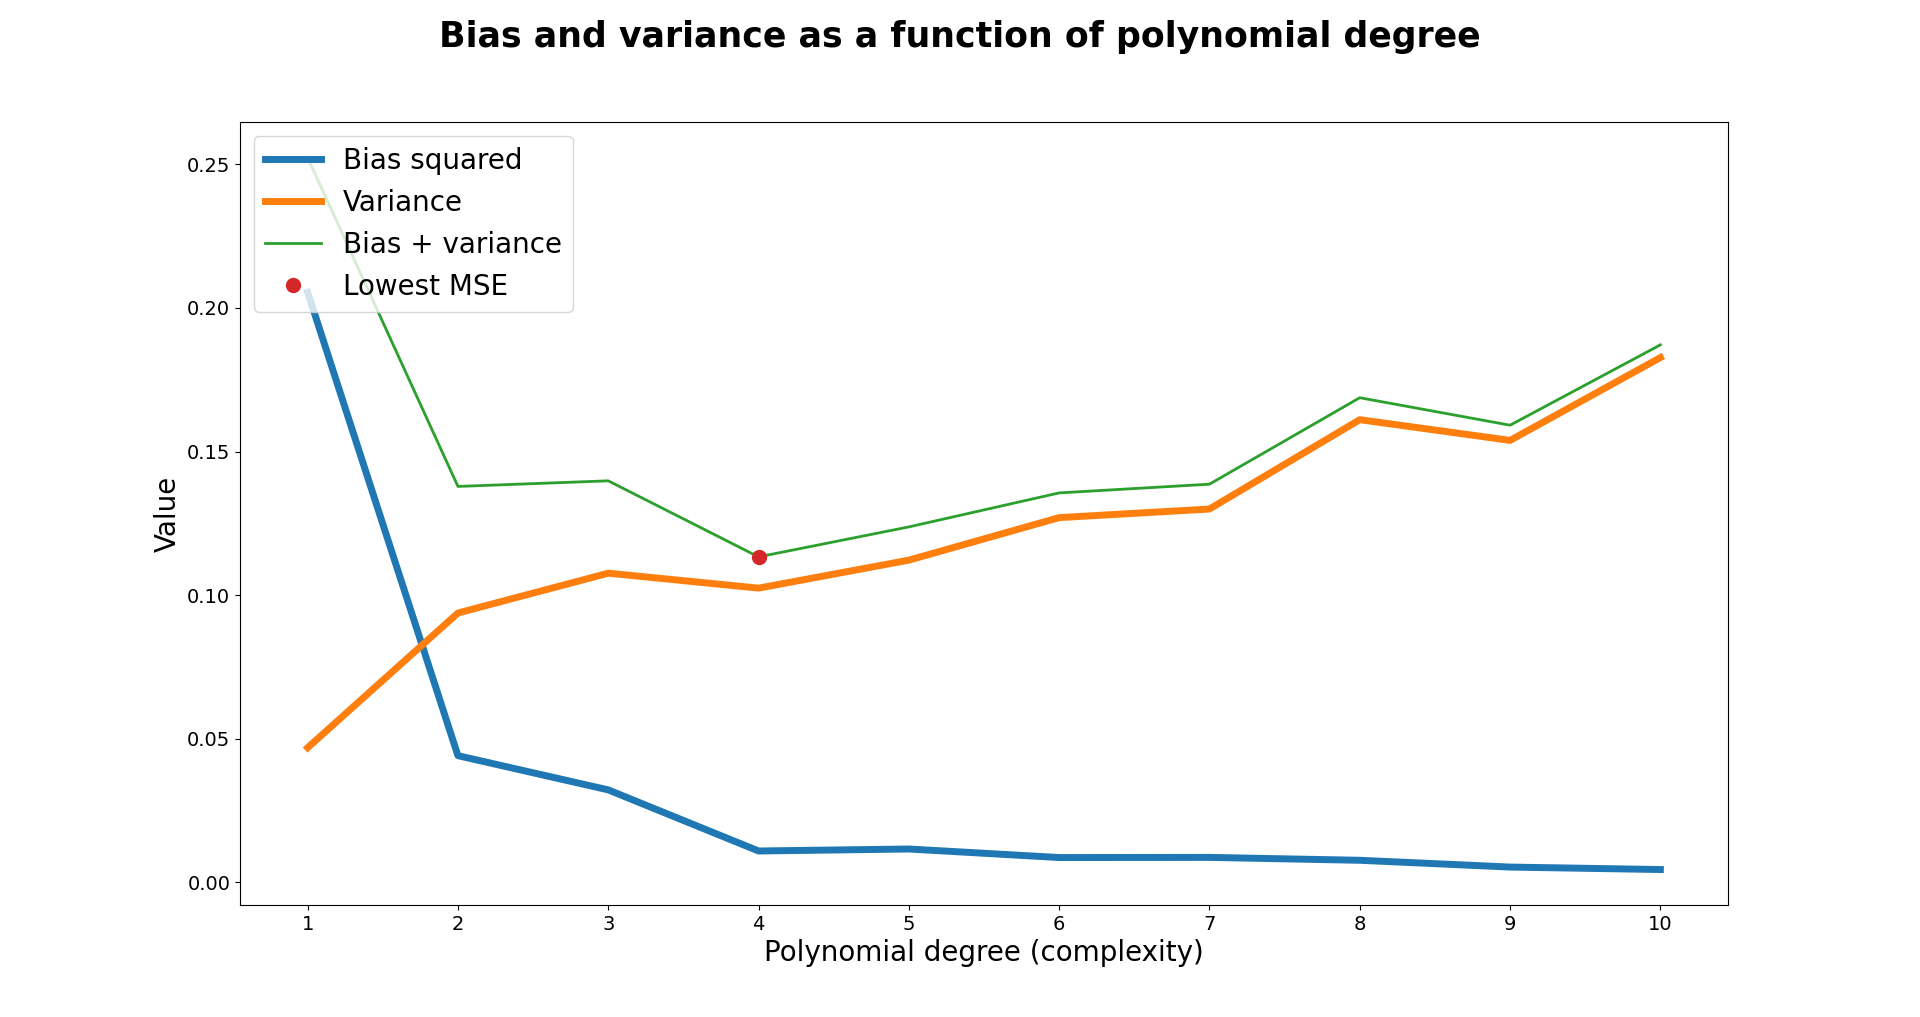
\includegraphics[width = 1\linewidth]{C:/Users/Sander/Documents/GitHub/FYS-STK4155/Project1/Report/Figures/BVplotCV_n100_p10_noise0001_CV5.PNG}
\caption{\label{fig:BVCV2} Bias and variance decomposition of figure \ref{fig:MSECV1}. The bias and variance change as a function of polynomial degree. Here we have 100 observations while we use 5-fold CV with a noise level of $0.001$.}
\end{figure}

\noindent What we observe when comparing figure \ref{fig:MSECV1} to figure \ref{fig:MSECV2} and figure \ref{fig:BVCV1} to figure \ref{fig:BVCV2} is that the bias looks the same, but the variance increases at a lower rate when using 5-fold CV rather than 10-fold CV. As a result, the MSE is lower at higher polynomials for the 5-fold CV, thus decreasing the risk of over-fitting. We can continue this examination by seeing what happens when we use LOOCV as in figure \ref{fig:MSECV3} and \ref{fig:BVCV3}

\begin{figure}[H]
\centering
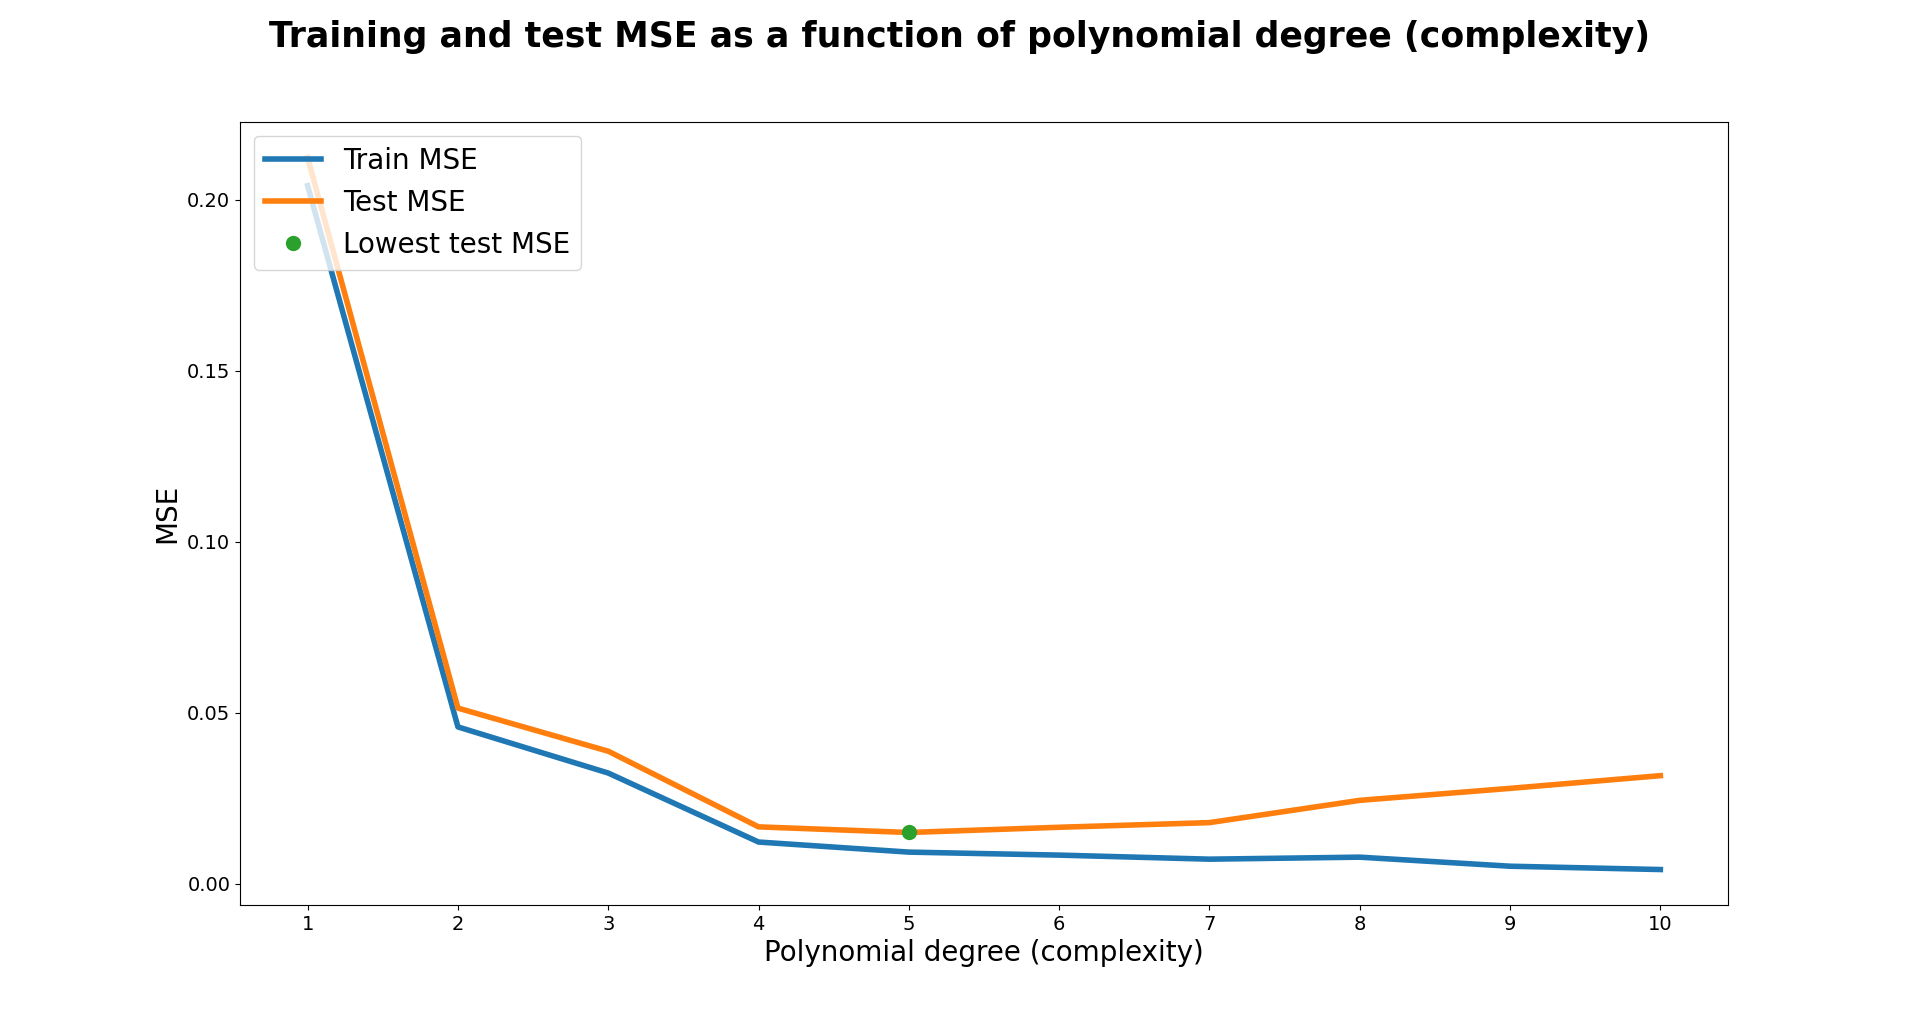
\includegraphics[width = 1\linewidth]{C:/Users/Sander/Documents/GitHub/FYS-STK4155/Project1/Report/Figures/MSECV_n100_p10_noise0001_CV1_shuffles.PNG}
\caption{\label{fig:MSECV3} MSE as a function of polynomial degree up to 10 using the LOOCV resampling method. Here we have 100 observations while we split the data into n different folds with a noise level of $0.001$.}
\end{figure}

\begin{figure}[H]
\centering
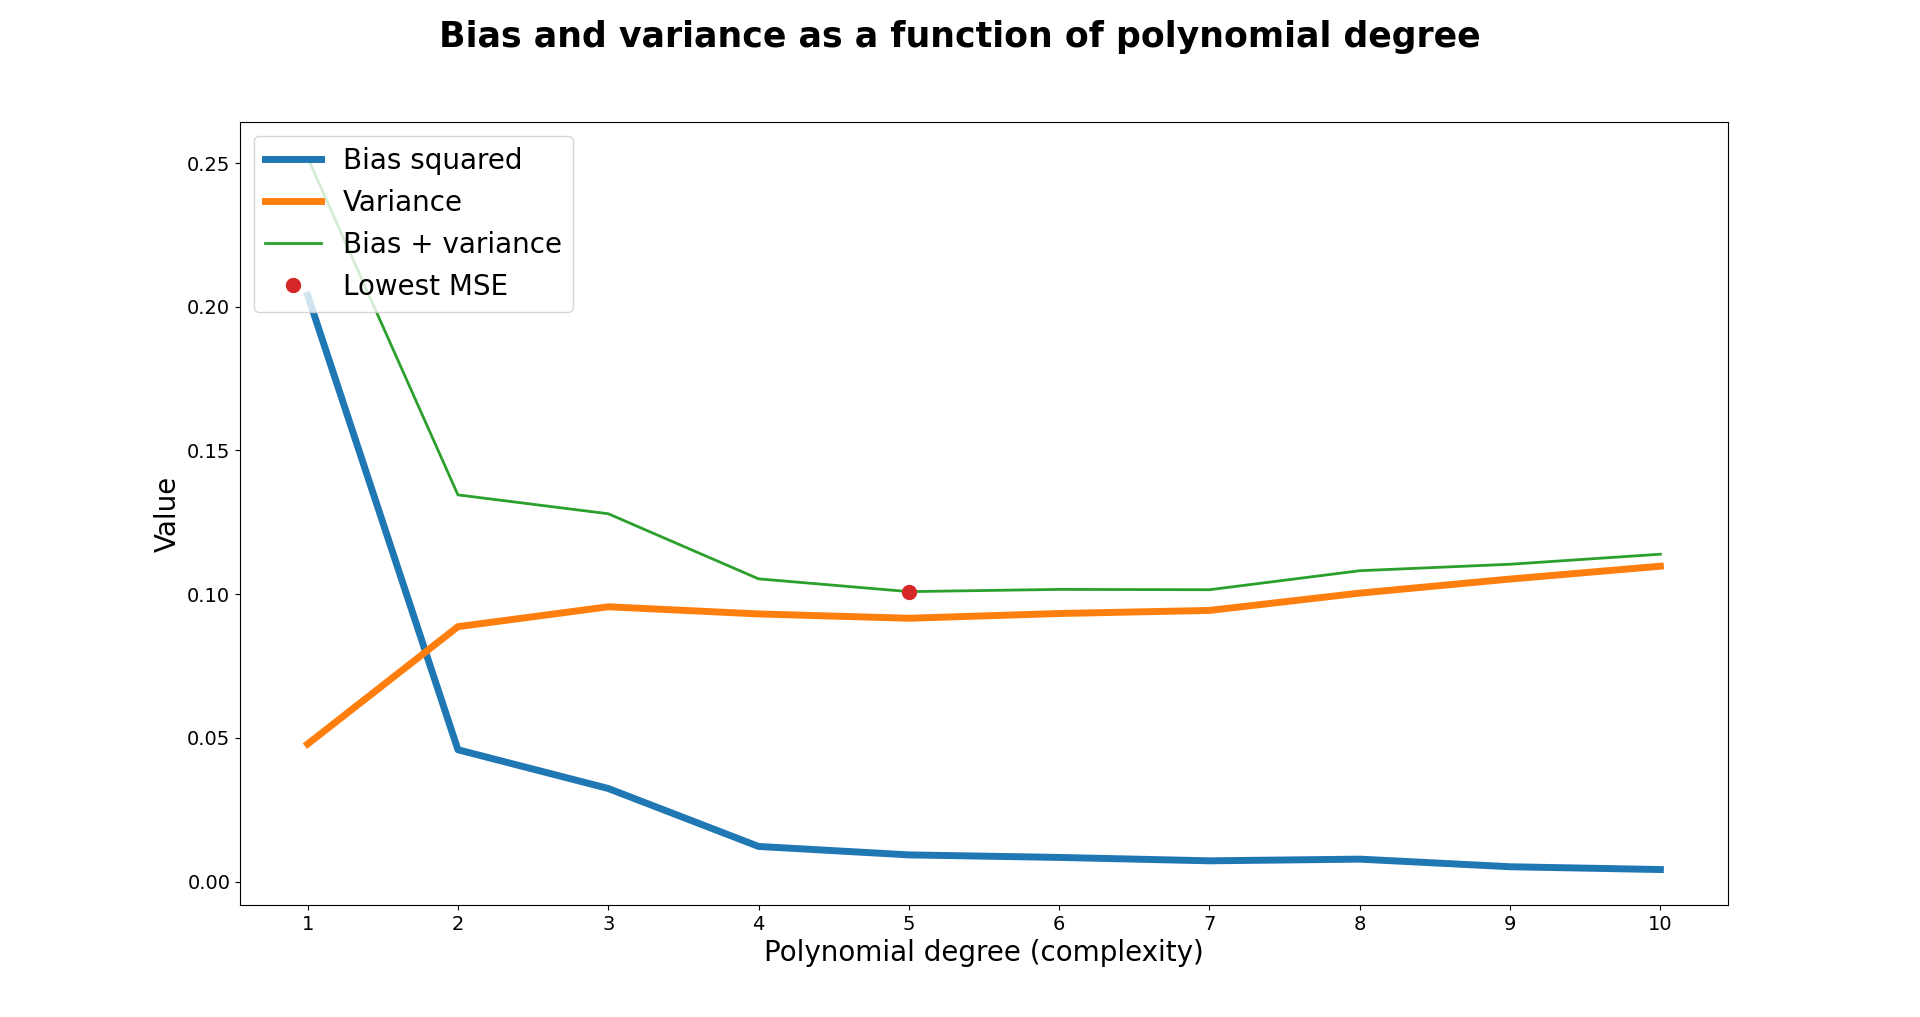
\includegraphics[width = 1\linewidth]{C:/Users/Sander/Documents/GitHub/FYS-STK4155/Project1/Report/Figures/BVplotCV_n100_p10_noise0001_CV1.PNG}
\caption{\label{fig:BVCV3} Bias and variance decomposition of figure \ref{fig:MSECV1}. Here we have 100 observations while we use LOOCV with a noise level of $0.001$.}
\end{figure}

\noindent Like previously discussed, the slope of the variance is less steep than that of the 10 and 5-fold CVs, and the MSE is therefore lower at higher polynomial degrees. The reason for this effect is that decreasing the fold size "creates more data out of thin air", and having more data means that we could fit higher order polynomials without over-fitting, as previously discussed. This is observed from figures \ref{fig:MSECV3} and \ref{fig:BVCV3} as the lowest MSE is located at $p = 5$ instead of $p = 4$ as seen for higher folds. The complexity of lowest MSE using LOOCV is similar to the MSE for the bootstrap resampling method in figure \ref{fig:MSEBOOT1}, but we can observe that the test MSE increases slower than that of the bootstrap model. This may be caused by how the two different methods work. The CV resampling method utilizes the existing information to its fullest by training the data for each permutation of the fold splits. This is unlike the bootstrap which simply increases the number of observations without taking into account the various permutations of the entire data.
\\
The two different methods seems to yield preferable results which strengthen our believe in the resampling methods. This allows us to proceed to other linear regression schemes in the coming exercises.

\newpage

\begin{center}
\Large{\textbf{Exercise d): Ridge regression}}
\end{center}

\begin{center}
\large{\textbf{Ridge regression MSE as function of model complexity using bootstrap}}
\end{center}

\noindent We have only utilized the ordinary least squares (OLS) regression scheme so far, but now we want to utilize two different shrinkage methods, namely the Ridge and Lasso regression schemes. We will start by looking at the Ridge regression scheme and then proceed to Lasso in the next exercise. 
\\
Shrinkage methods like Ridge aim to find which variables are significant and which variables are not, and then removing the influence of the insignificant variables by either setting them to zero (Lasso) or close to zero (Ridge). This is done by adding the shrinkage parameter $\lambda$ to both sides of the OLS equation (equation \ref{eq:LinReg}) such that (Hastie, T., et al.,2009, [B])

\begin{equation}\label{eq:RidgeDerive}
\begin{aligned}
\boldsymbol{\hat{y}}_{Ridge} + \lambda |\boldsymbol{\beta}|^2 = \textbf{X}\boldsymbol{\beta} + \lambda  |\boldsymbol{\beta}|^2
\end{aligned}
\end{equation}

\noindent Solving equation \ref{eq:RidgeDerive} for the regression coefficients $\boldsymbol{\beta}$ with respects to minimizing the residual sum of squares yields (Hastie, T., et al., [B])

\begin{equation}\label{eq:RidgeDerive2}
\begin{aligned}
\boldsymbol{\hat{\beta}} = (\textbf{X}^T \textbf{X} + \lambda \textbf{I})^{-1} \textbf{X}^T \boldsymbol{\hat{y}}_{Ridge}
\end{aligned}
\end{equation}

\noindent Where $\textbf{I}$ is the identity matrix. We can then repeat the analysis of exercises a through c, but this time using equation \ref{eq:RidgeDerive2} to train the data. 
\\
First let us investigate how the MLE of the Ridge regression changes as a function of different polynomial degrees. If we again repeat the exact experiment as in exercise b), that is a original data set consisting of 100 observations, a noise level of $0.001$, a train/test split of $75/25$ and with 100 bootstrap iterations we obtain figure \ref{fig:MSERidgeBoot3}

\begin{figure}[H]
\centering
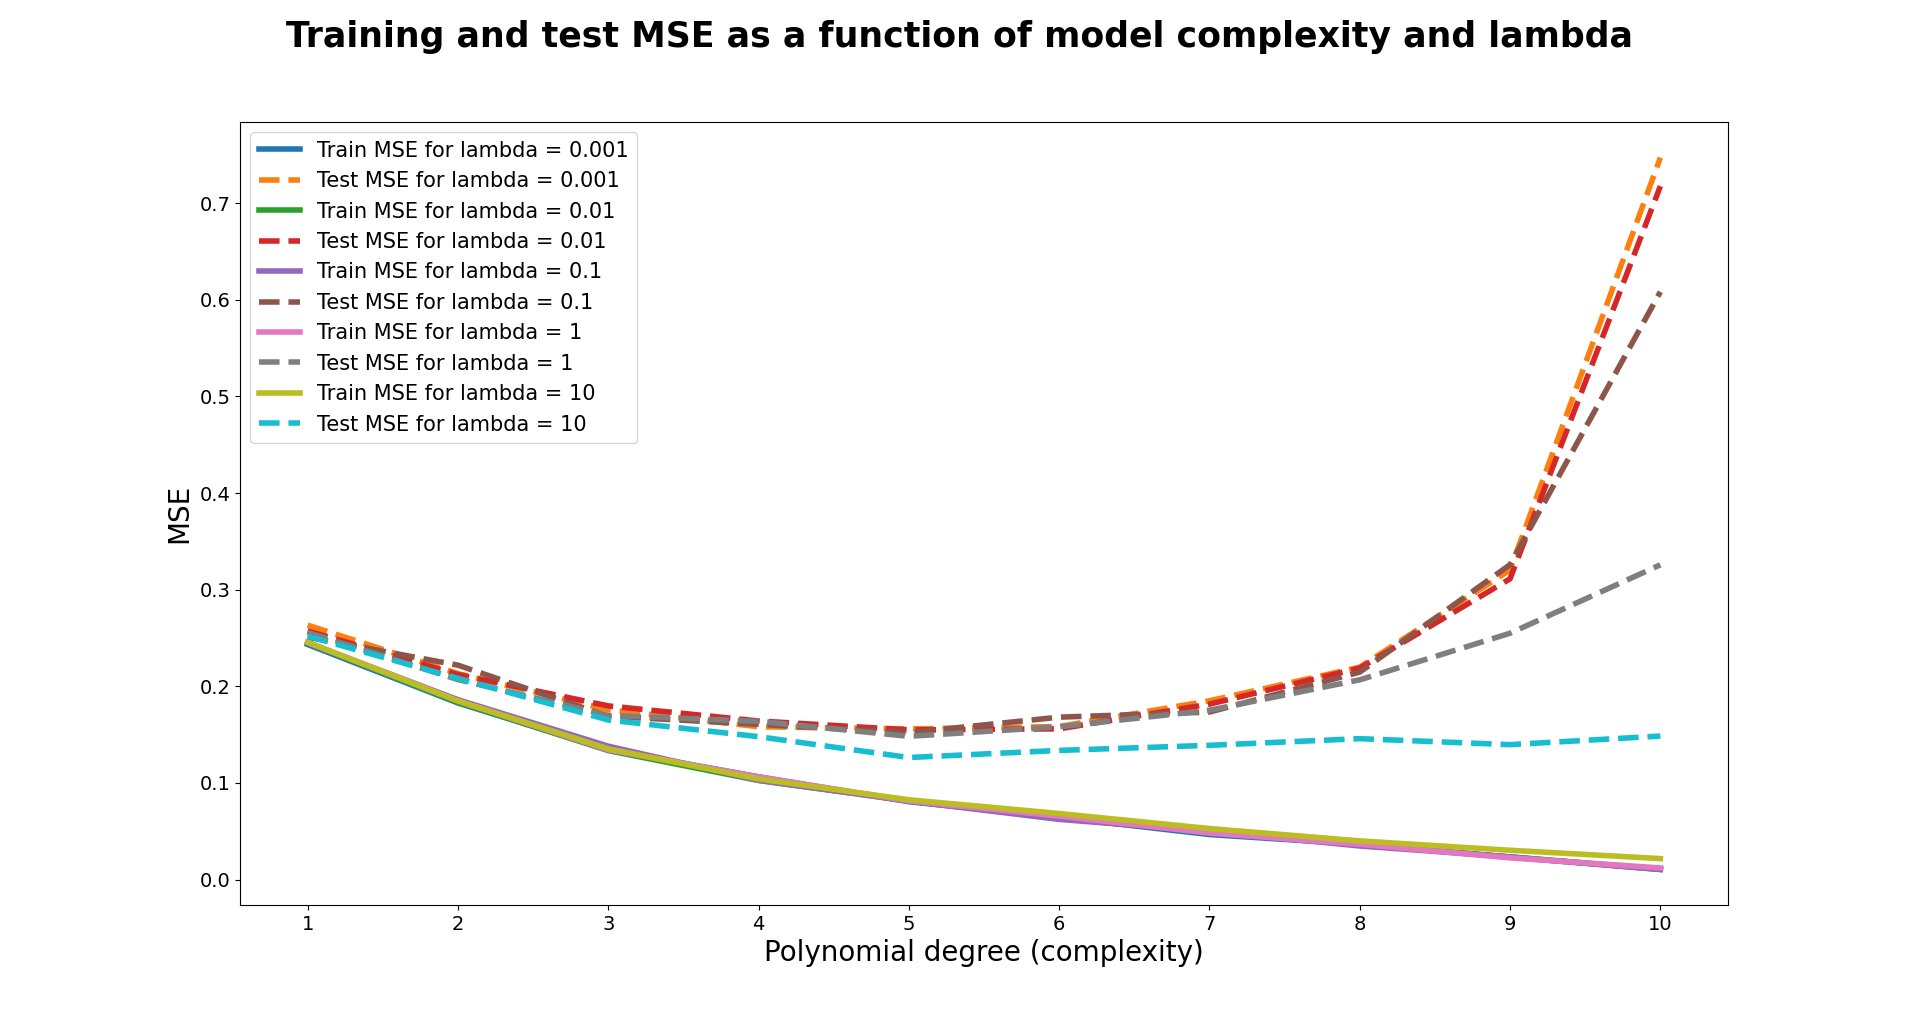
\includegraphics[width = 1\linewidth]{C:/Users/Sander/Documents/GitHub/FYS-STK4155/Project1/Report/Figures/MSEBOOT_n100_p10_noise0001_B100_RIDGE.PNG}
\caption{\label{fig:MSERidgeBoot3} MSE as a function of polynomial degree up to 10 for different values of $\lambda$ using the bootstrap resampling method with 100 iterations. Here we have 100 observations while we split the data into $75/25$ train/test split with a noise level of $0.001$.}
\end{figure}

\noindent It can be observed from figure \ref{fig:MSERidgeBoot3} that the training MSE goes towards zero regardless of the $\lambda$-value. The test MSE initially decreases to some value of p, but will eventually start to increase. The increase seems to be dependent on the value of $\lambda$, as lower values seem to increase faster than the higher values of $\lambda$. We can observe that the test MSE for $\lambda = 10$ never seems to increase, while the test MSE for $\lambda = 0.001$ seems to increase drastically after $p = 5$. Again, it seems that $p = 5$ is the polynomial degree of minimum MSE. We can decompose figure \ref{fig:MSERidgeBoot3} into its bias and variance components as done in figure \ref{fig:BVRidge1}

\begin{figure}[H]
\centering
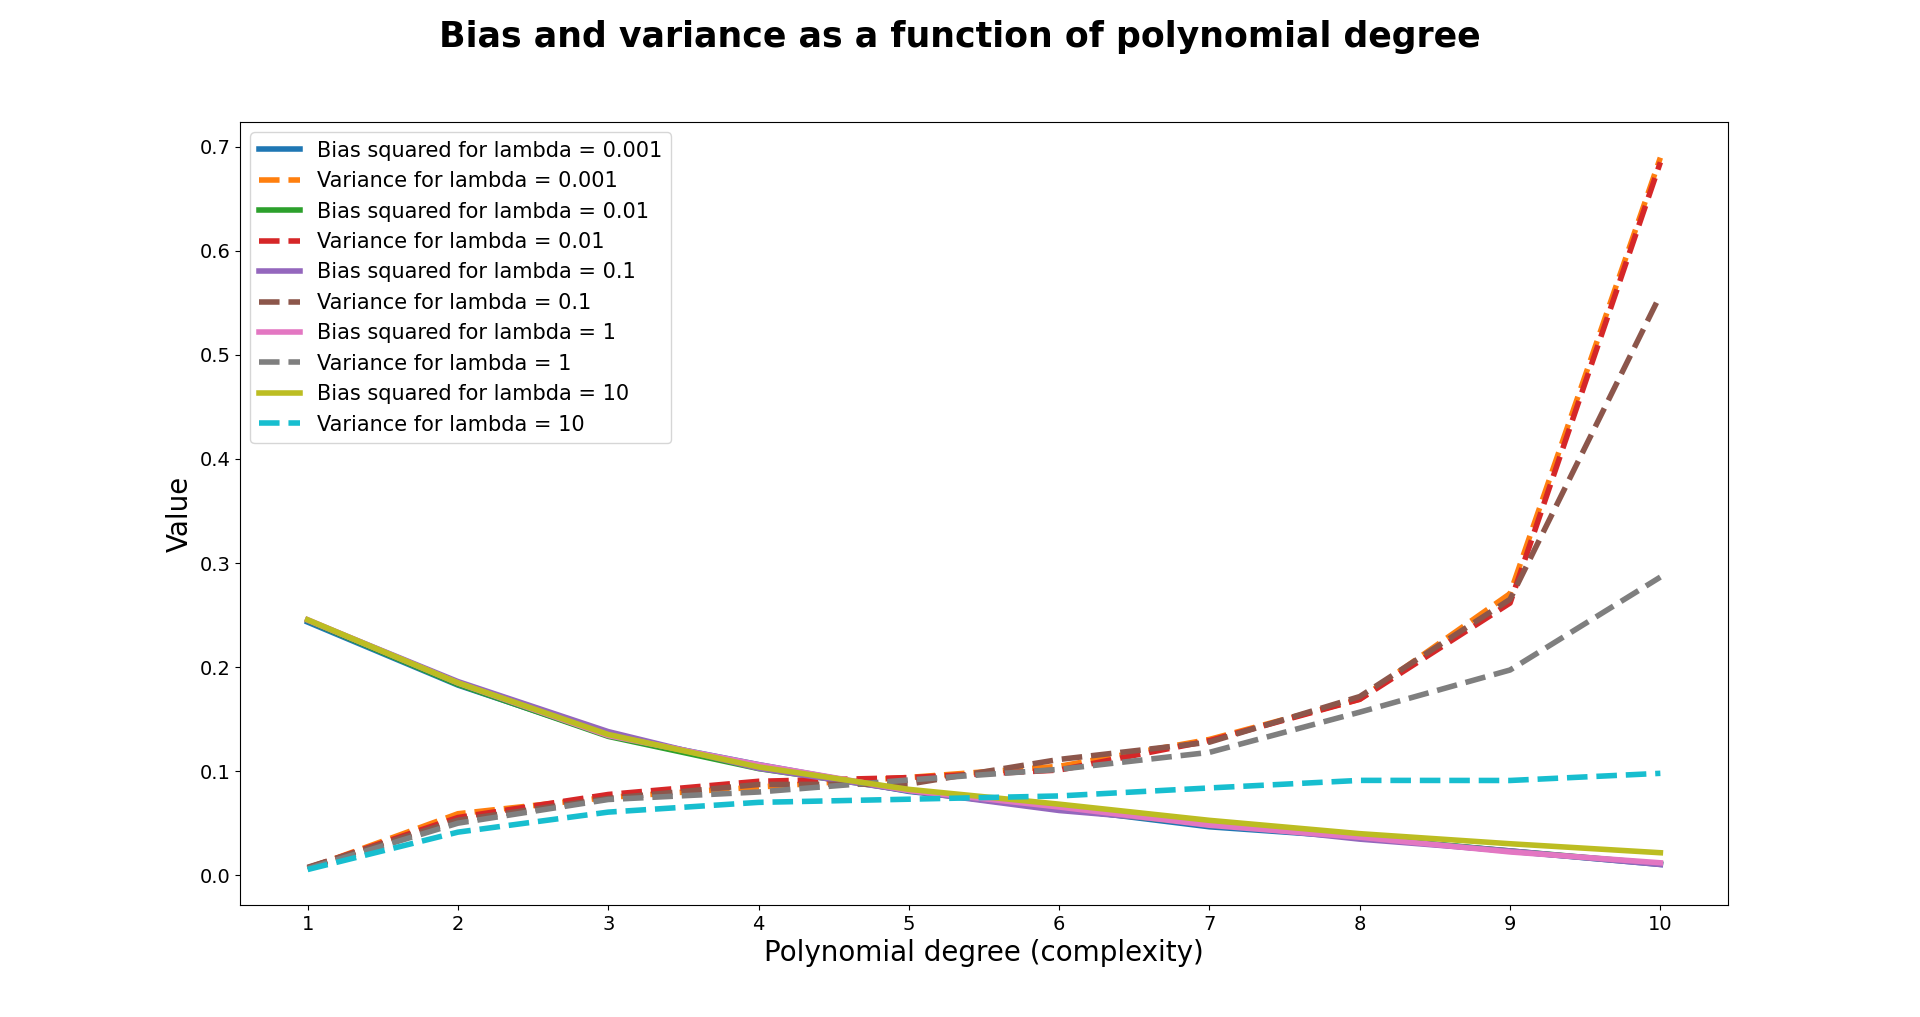
\includegraphics[width = 1\linewidth]{C:/Users/Sander/Documents/GitHub/FYS-STK4155/Project1/Report/Figures/BVplotBOOT_n100_p10_noise0001_ts025_B100_RIDGE.PNG}
\caption{\label{fig:BVRidge1} Bias and variance decomposition of figure \ref{fig:MSERidgeBoot3}. The bias and variance change as a function of polynomial degree and values of $\lambda$ using the bootstrap resampling method. Here we have 100 observations while we use a $75/25$ train/test split with a noise level of $0.001$.}
\end{figure}

\noindent We can observe from figure \ref{fig:BVRidge1} that the bias always decreases as previously seen in exercise b) (figure \ref{fig:BVBOOT1}). However, the variance seem to depend on both the complexity of our model and the value of $\lambda$. Figure \ref{fig:BVRidge1} confirms what we previously saw in figure \ref{fig:MSERidgeBoot3}, namely that lower values of $\lambda$ yields higher variance as a function of complexity, thus yielding a higher MSE.

\begin{center}
\large{\textbf{Regression coefficients as function of $\lambda$ using bootstrap}}
\end{center}

\noindent The next step is to see what happens with the beta coefficients when we apply different values of $\lambda$ to equation \ref{eq:RidgeDerive2}. We can plot the regression coefficient values for a given range of shrinkage parameters and see how the value changes. Here we have chosen the $\lambda$-values as $[0.00001, 0.0001, 0.001, 0.01, 0.1, 1, 10, 100, 1000, 10000, 100000]$ where we use polynomials up to degree 5. The result is plotted in figure \ref{fig:LambdaPlot1}

\begin{figure}[H]
\centering
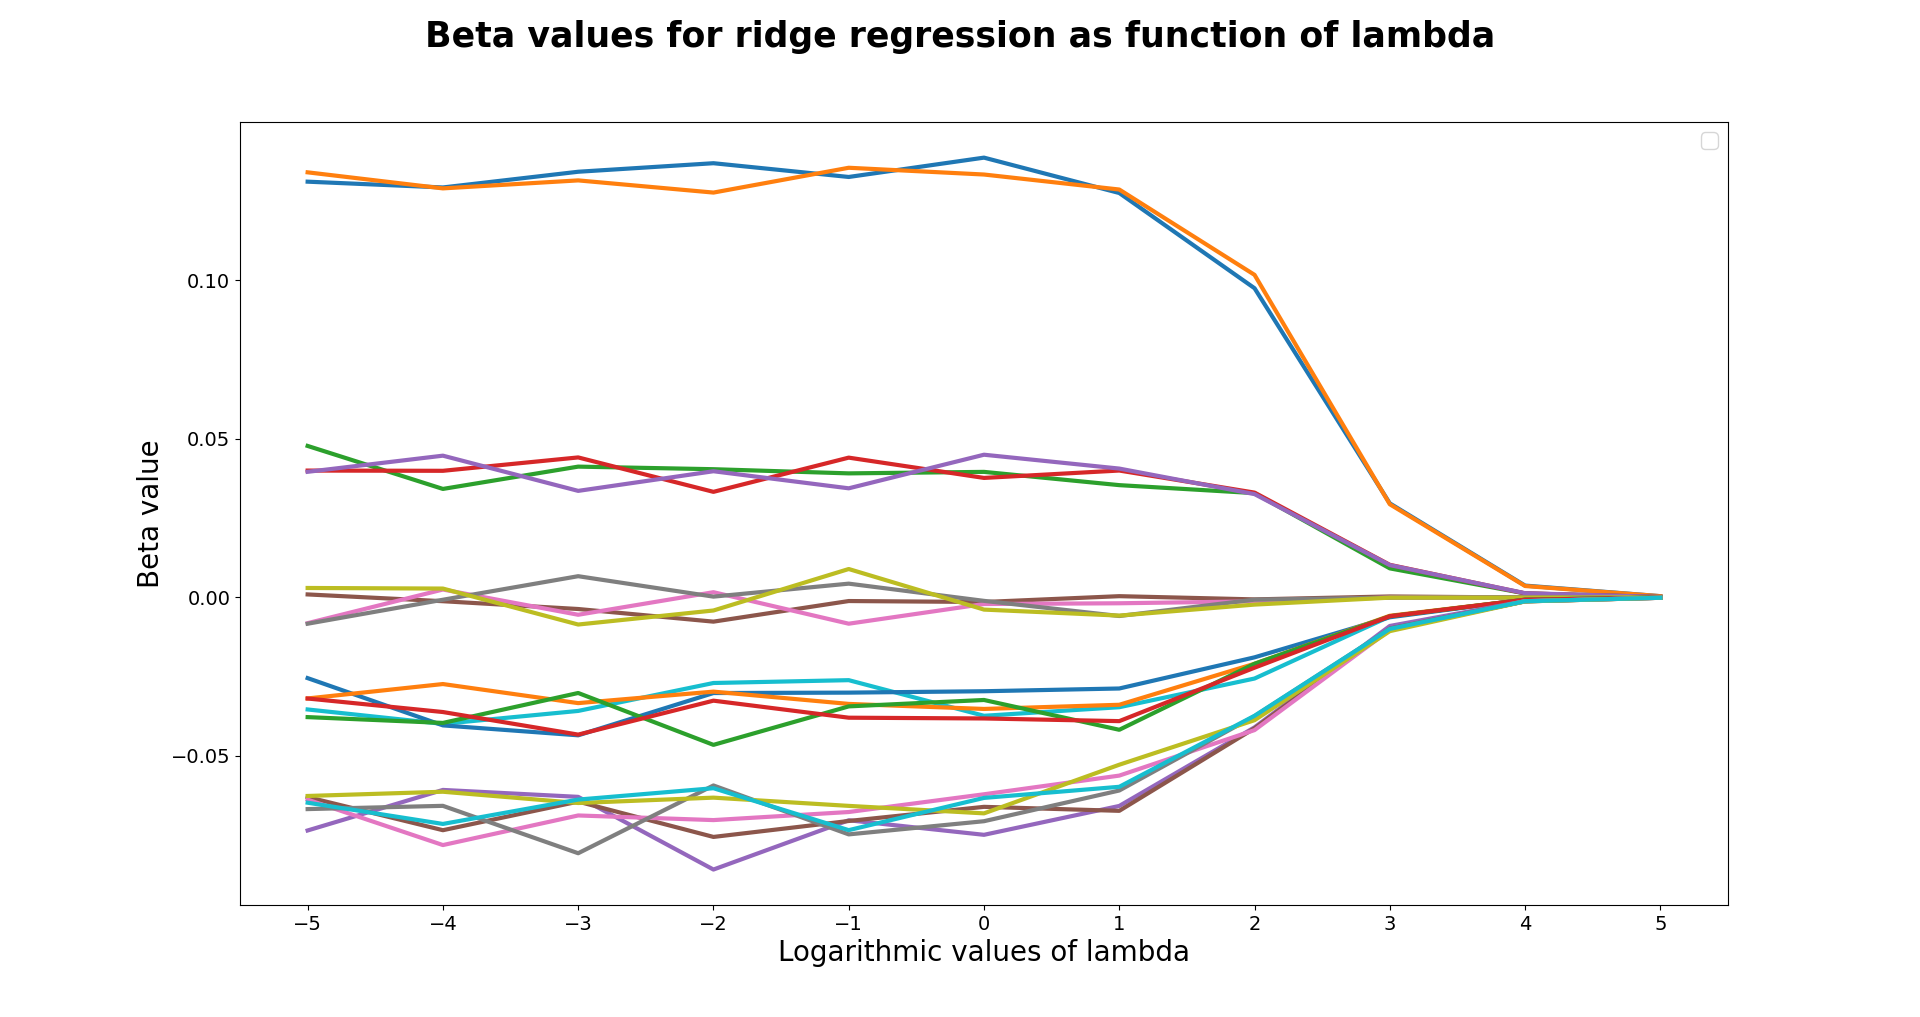
\includegraphics[width = 1\linewidth]{C:/Users/Sander/Documents/GitHub/FYS-STK4155/Project1/Report/Figures/LambdaPlot_n100_p5_noise0001_ts025_B100_RIDGE.PNG}
\caption{\label{fig:LambdaPlot1} Regression coefficient values of up to $p = 5$ as function of logarithmic $\lambda$-value using the bootstrap method with 100 iterations. The original dataset is of size 100.}
\end{figure}

\noindent It is difficult to see any trends as we have so many regression coefficients and we therefore sort figure \ref{fig:LambdaPlot1} into its different polynomial degrees such that first order polynomials ($x,y$) have one color and second order polynomial ($xy,x^2,y^2$) have another color and so on. The resulting plot is shown in figure \ref{fig:LambdaPlot2}

\begin{figure}[H]
\centering
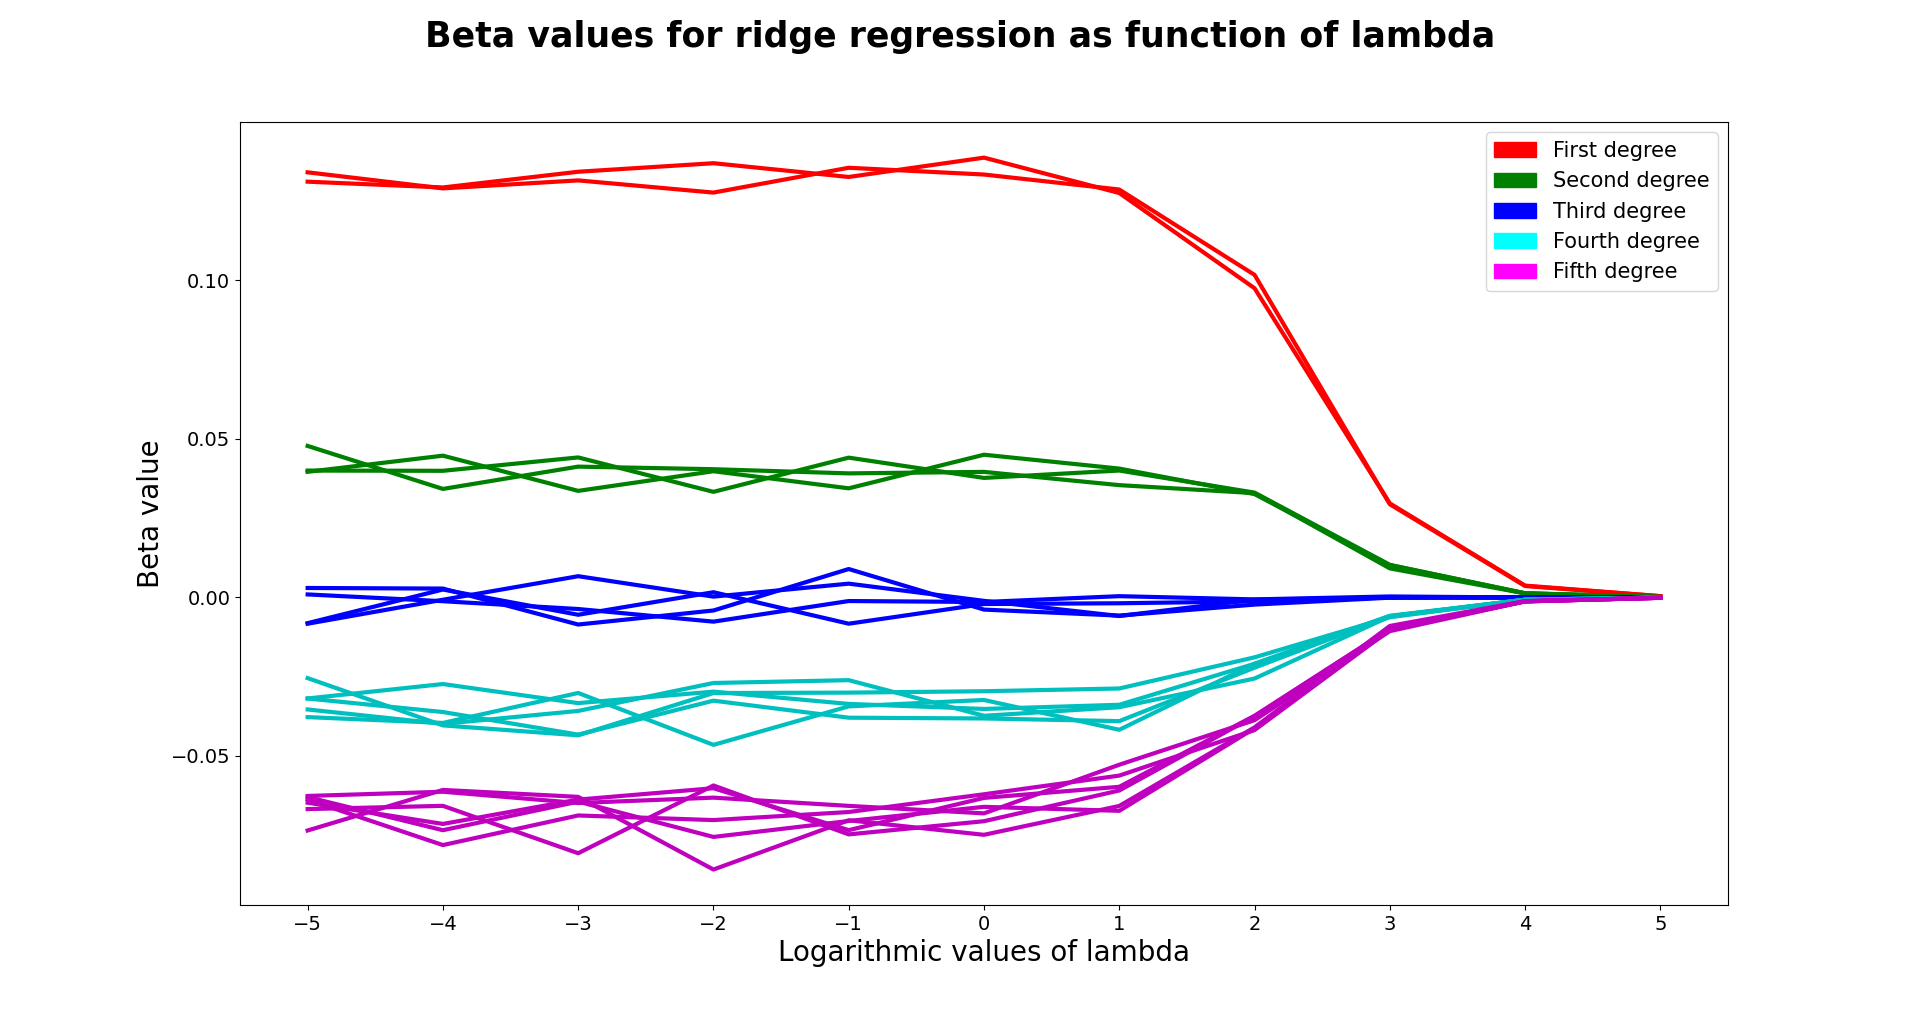
\includegraphics[width = 1\linewidth]{C:/Users/Sander/Documents/GitHub/FYS-STK4155/Project1/Report/Figures/LambdaPlot_n100_p5_noise0001_ts025_B100_RIDGESort.PNG}
\caption{\label{fig:LambdaPlot2} Regression coefficient values of up to $p = 5$ as function of logarithmic $\lambda$-value using the bootstrap method with 100 iterations. The original dataset is of size 100. Here we have sorted polynomials of the same degree into the same color}
\end{figure}

\noindent From figure \ref{fig:LambdaPlot2} we can observe that the Ridge regression treats different polynomial degree unevenly. Much of the point of the ridge regression is to reduce the the variables in the design matrix towards zero, depending on their statistical significance. The higher the $\lambda$-values, the more variables will be reduced towards zero, but not exactly zero. We can observe this by comparing the third and first degree polynomial in figure \ref{fig:LambdaPlot2}. The third degree polynomial is reduced to a value close to zero at around $10^{-2} = 0.1$, while the first degree polynomial does not approach zero before $10^2 = 100$. This means that the ridge regression algorithm deems third degree polynomials as less significant than that of the first order polynomials. We can extend this though process and see that all variables will be reduced closed to zero (regardless of their polynomial degree) if $\lambda$ is large enough.

\begin{center}
\large{\textbf{MSE as function of model complexity using cross-validation}}
\end{center}

\noindent Let us now explore the CV resampling approach. We implement the CV algorithm the same way as in exercise c) and we investigate how the MSE changes as function of model complexity. We will use the exact same parameters as previously with $n = 100$ observations in the original data set, a noise-level of $0.001$ and 10 polynomial degrees. Furthermore, we want to try the 10-fold, 5-fold and leave-one-out cross-validations and see what the difference between the outcomes are. The MSE versus polynomial degree is plotted for each CV-type in figure \ref{fig:MSERidgeCV1}, \ref{fig:MSERidgeCV2} and \ref{fig:MSERidgeCV3}

\begin{figure}[H]
\centering
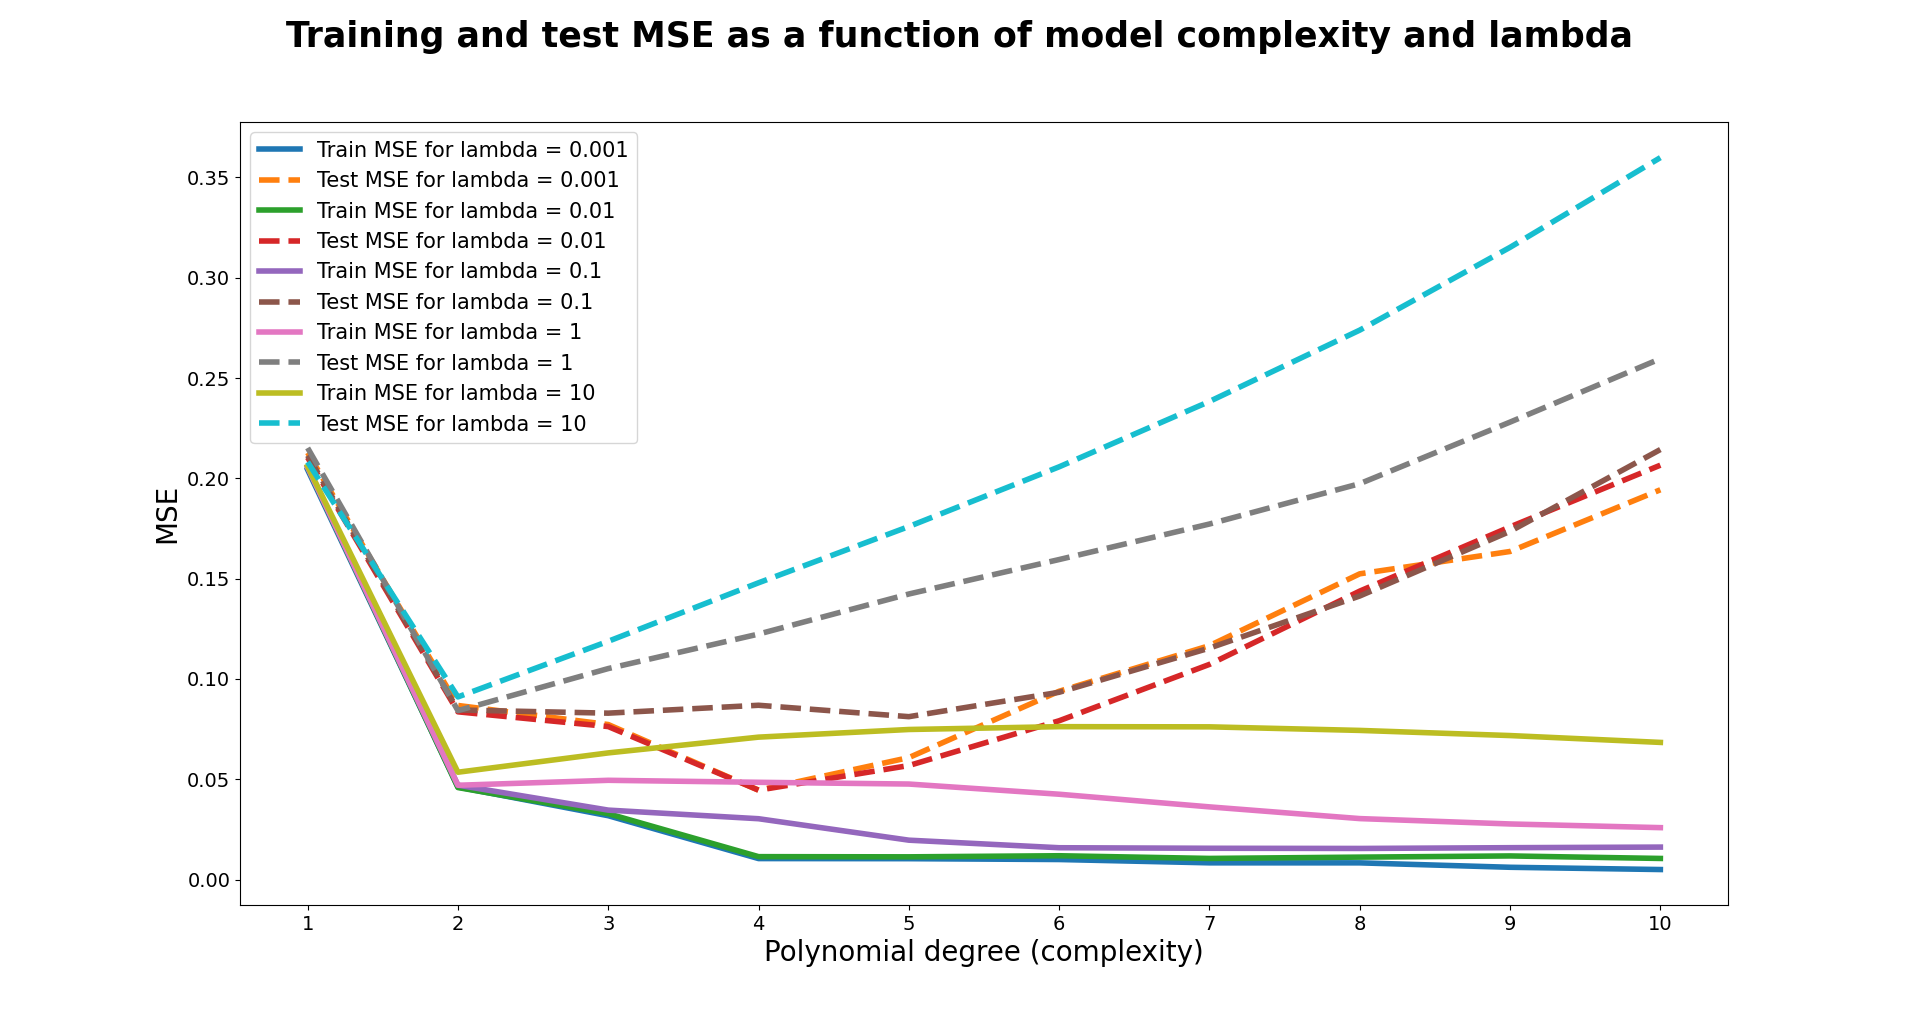
\includegraphics[width = 1\linewidth]{C:/Users/Sander/Documents/GitHub/FYS-STK4155/Project1/Report/Figures/MSECV_n100_p10_noise0001_CV10_RIDGE.PNG}
\caption{\label{fig:MSERidgeCV1} MSE as a function of polynomial degree up to 10 for different values of $\lambda$ using the 10-fold CV resampling method. Here we have 100 observations while we consider every possible permutation of a 10-fold cross-validation with a noise level of $0.001$.}
\end{figure}

\begin{figure}[H]
\centering
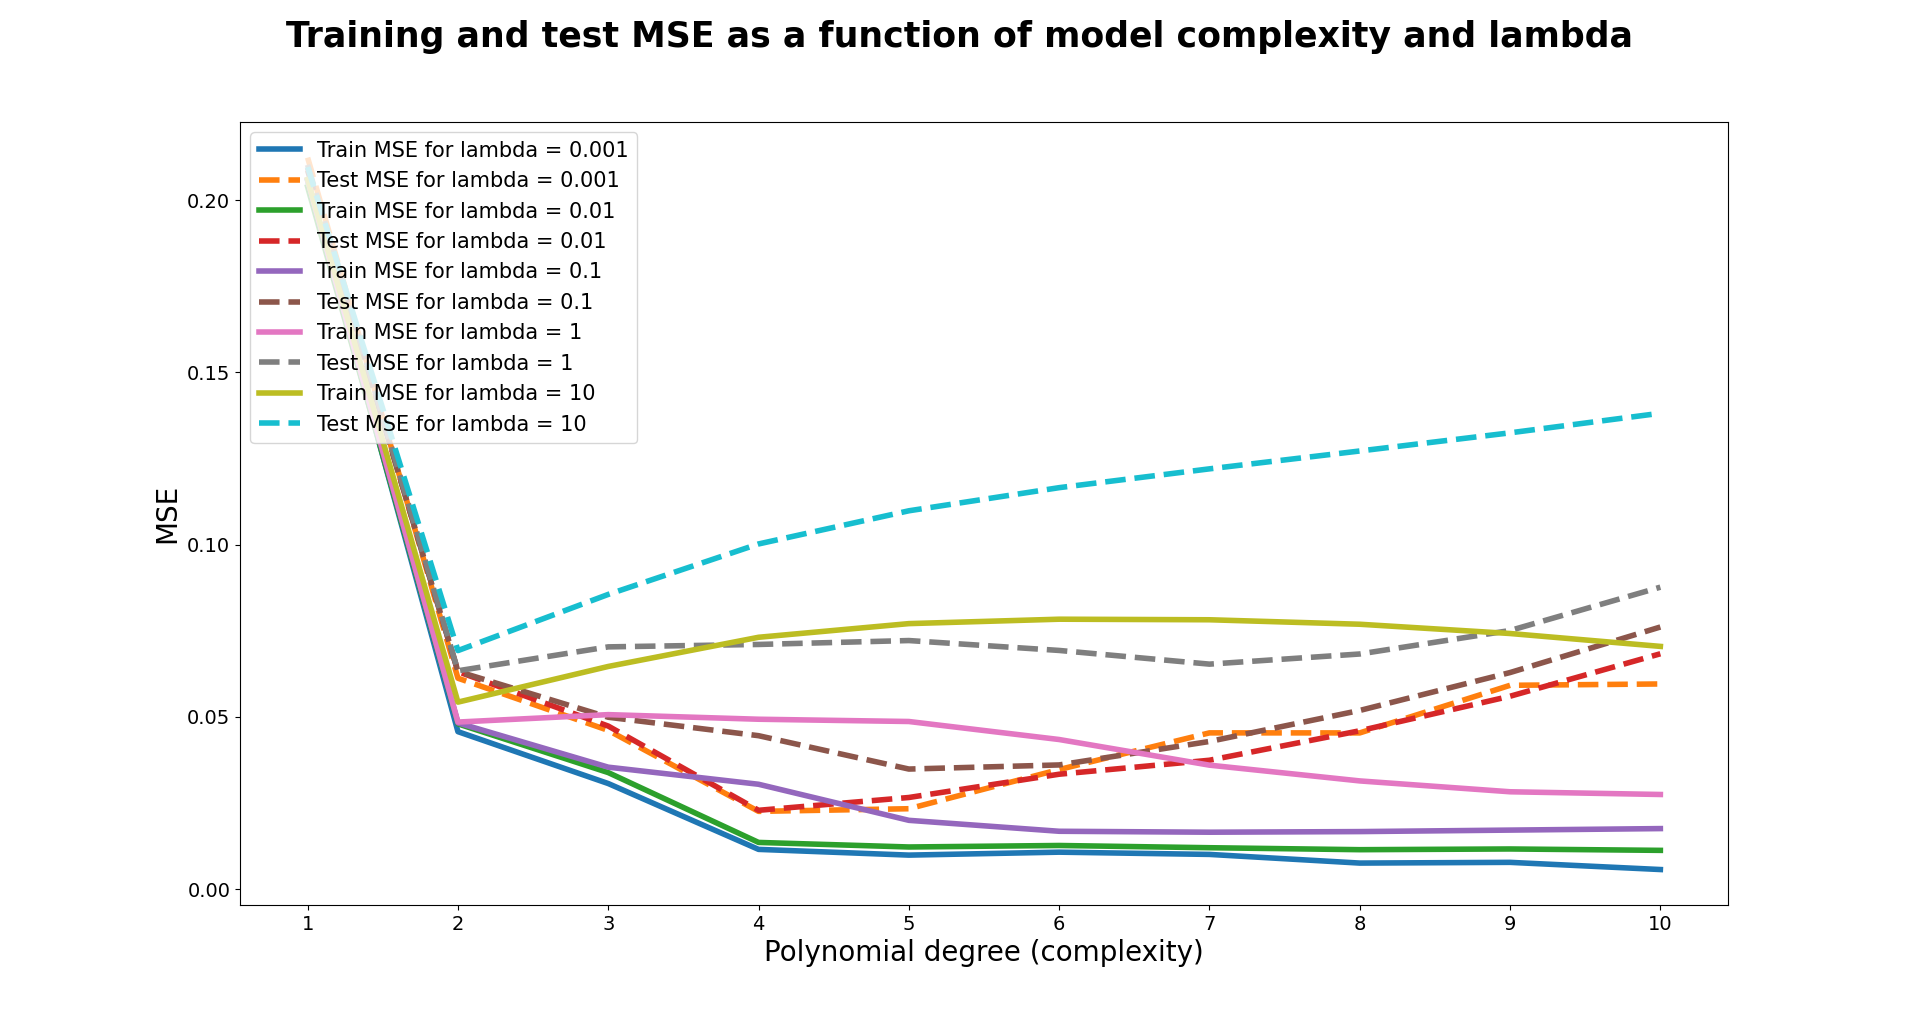
\includegraphics[width = 1\linewidth]{C:/Users/Sander/Documents/GitHub/FYS-STK4155/Project1/Report/Figures/MSECV_n100_p10_noise0001_CV5_RIDGE.PNG}
\caption{\label{fig:MSERidgeCV2} MSE as a function of polynomial degree up to 10 for different values of $\lambda$ using the 5-fold CV resampling method. Here we have 100 observations while we consider every possible permutation of a 5-fold cross-validation with a noise level of $0.001$.}
\end{figure}

\begin{figure}[H]
\centering
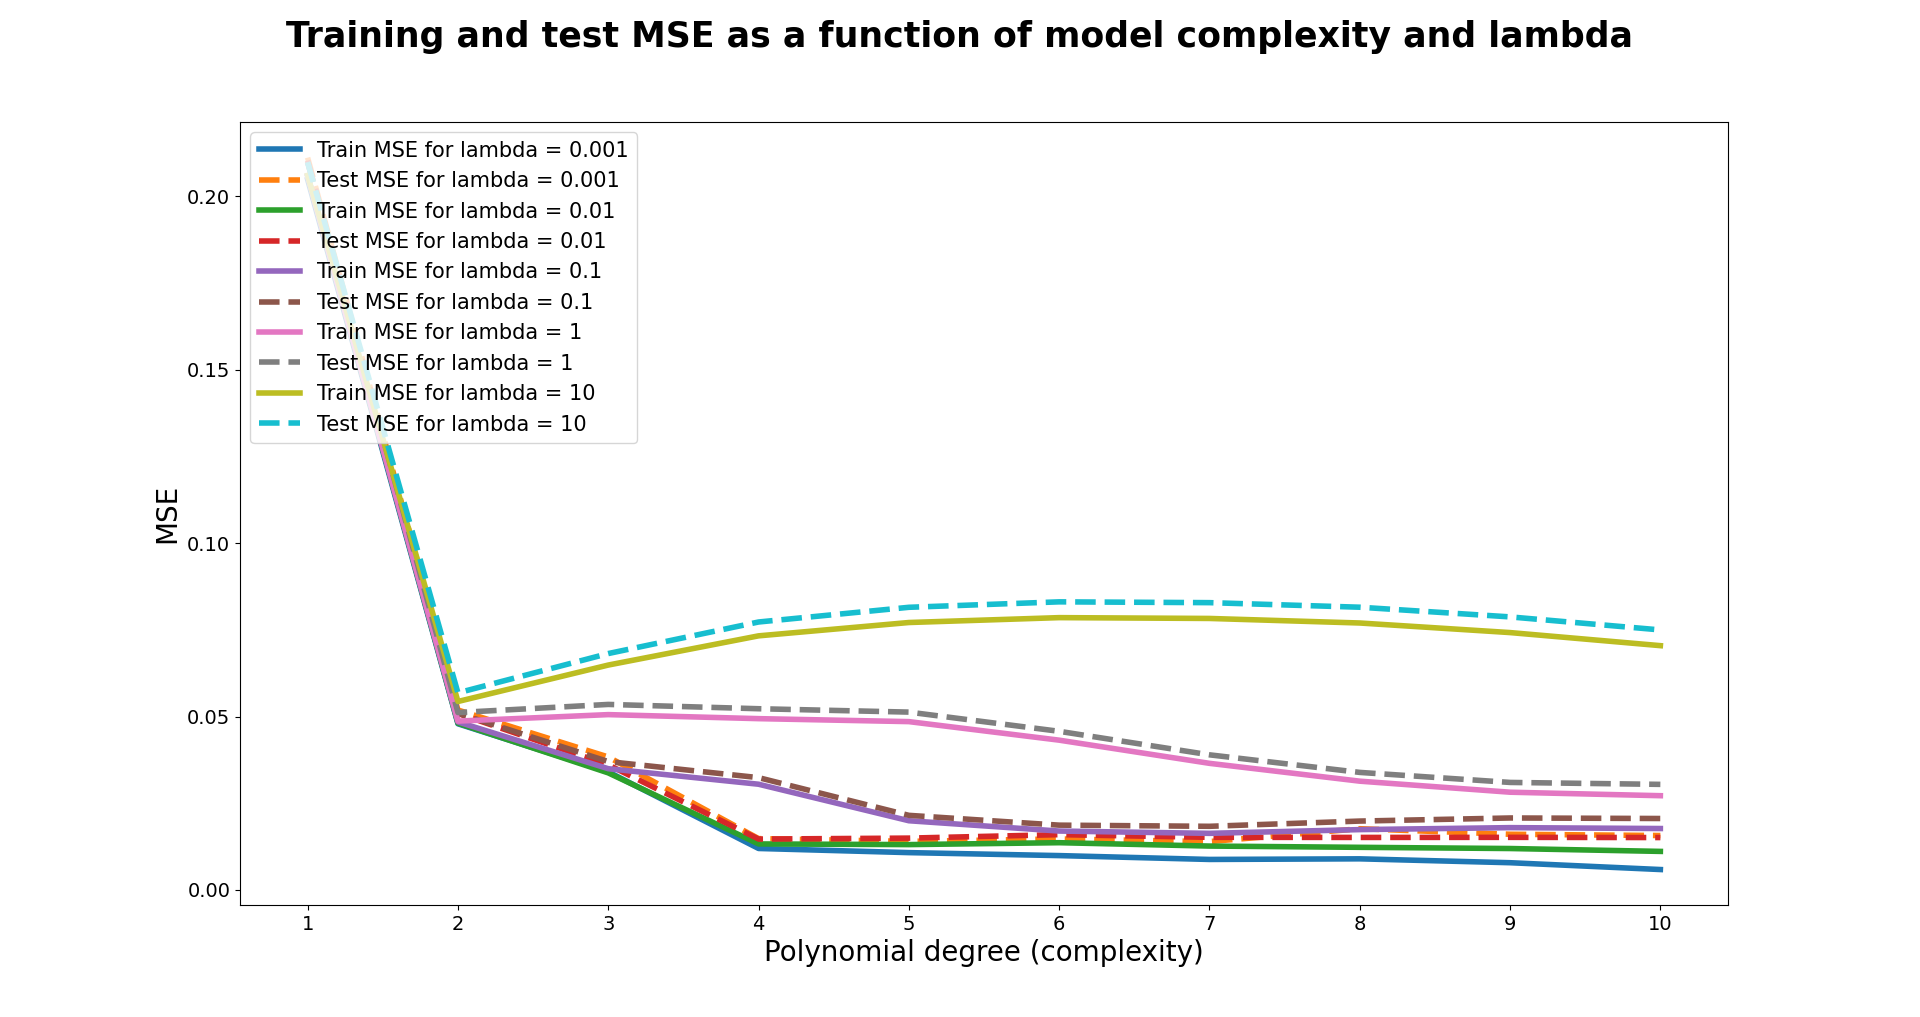
\includegraphics[width = 1\linewidth]{C:/Users/Sander/Documents/GitHub/FYS-STK4155/Project1/Report/Figures/MSECV_n100_p10_noise0001_CV1_RIDGE.PNG}
\caption{\label{fig:MSERidgeCV3} MSE as a function of polynomial degree up to 10 for different values of $\lambda$ using the leave-one-out CV resampling method. Here we have 100 observations while we consider every possible permutation of a leave-one-out cross-validation with a noise level of $0.001$.}
\end{figure}

\noindent One can observe from figures \ref{fig:MSERidgeCV1}, \ref{fig:MSERidgeCV2} and \ref{fig:MSERidgeCV3} that the MSEs rapidly decrease from 1 to 2 polynomial degrees. After $p = 2$ however, some models increase in MSE while others decrease. We observe that $\lambda$-values larger than 1 are the models that increase their MSE at $p = 2$, while models using $\lambda$-values between 0 and 1 tend to decrease further after $p = 2$. This means means that $\lambda$ should be chosen as somewhere in between 0 and 1, as the test MSE is lowest here.
\\
What is also observed from figures \ref{fig:MSERidgeCV1}, \ref{fig:MSERidgeCV2} and \ref{fig:MSERidgeCV3} is that the training MSE for some models, namely those of higher values of $\lambda$, do not approach zero imminently. This is due to the Ridge regression reducing some of the variables to zero (least significant ones) which actually lowers the MSE of even the training data. This was not a problem when we used OLS or bootstrap resampling, meaning the CV resampling method is more sensitive to which variables are considered in the regression. 
\\
Another interesting observations is that decreasing the fold size tend to decrease the MSE. When we compare figures \ref{fig:MSERidgeCV1}, \ref{fig:MSERidgeCV2} and \ref{fig:MSERidgeCV3} we see that the LOOCV has the lowest overall MSE while the 10-fold CV has the highest overall MSE. This is not surprising as using smaller folds sizes inherently "creates" more data, allowing for larger polynomial degrees to yield lower MSEs. In fact, we can see that for the LOOCV case (figure \ref{fig:MSERidgeCV3}), some of the models never really increase their test MSE for polynomials up to 10th order. This means that creating $n^2$ amount of data allows us to create models with much higher order of polynomials. This means further that we can more accurately predict responses by using higher order polynomials in our model when utilizing LOOCV.
\\
We can decompose the test MSEs from figures \ref{fig:MSERidgeCV1}, \ref{fig:MSERidgeCV2} and \ref{fig:MSERidgeCV3} into their bias and variance components as done in figures \ref{fig:BVRidgeCV1}, \ref{fig:BVRidgeCV2} and \ref{fig:BVRidgeCV3}

\begin{figure}[H]
\centering
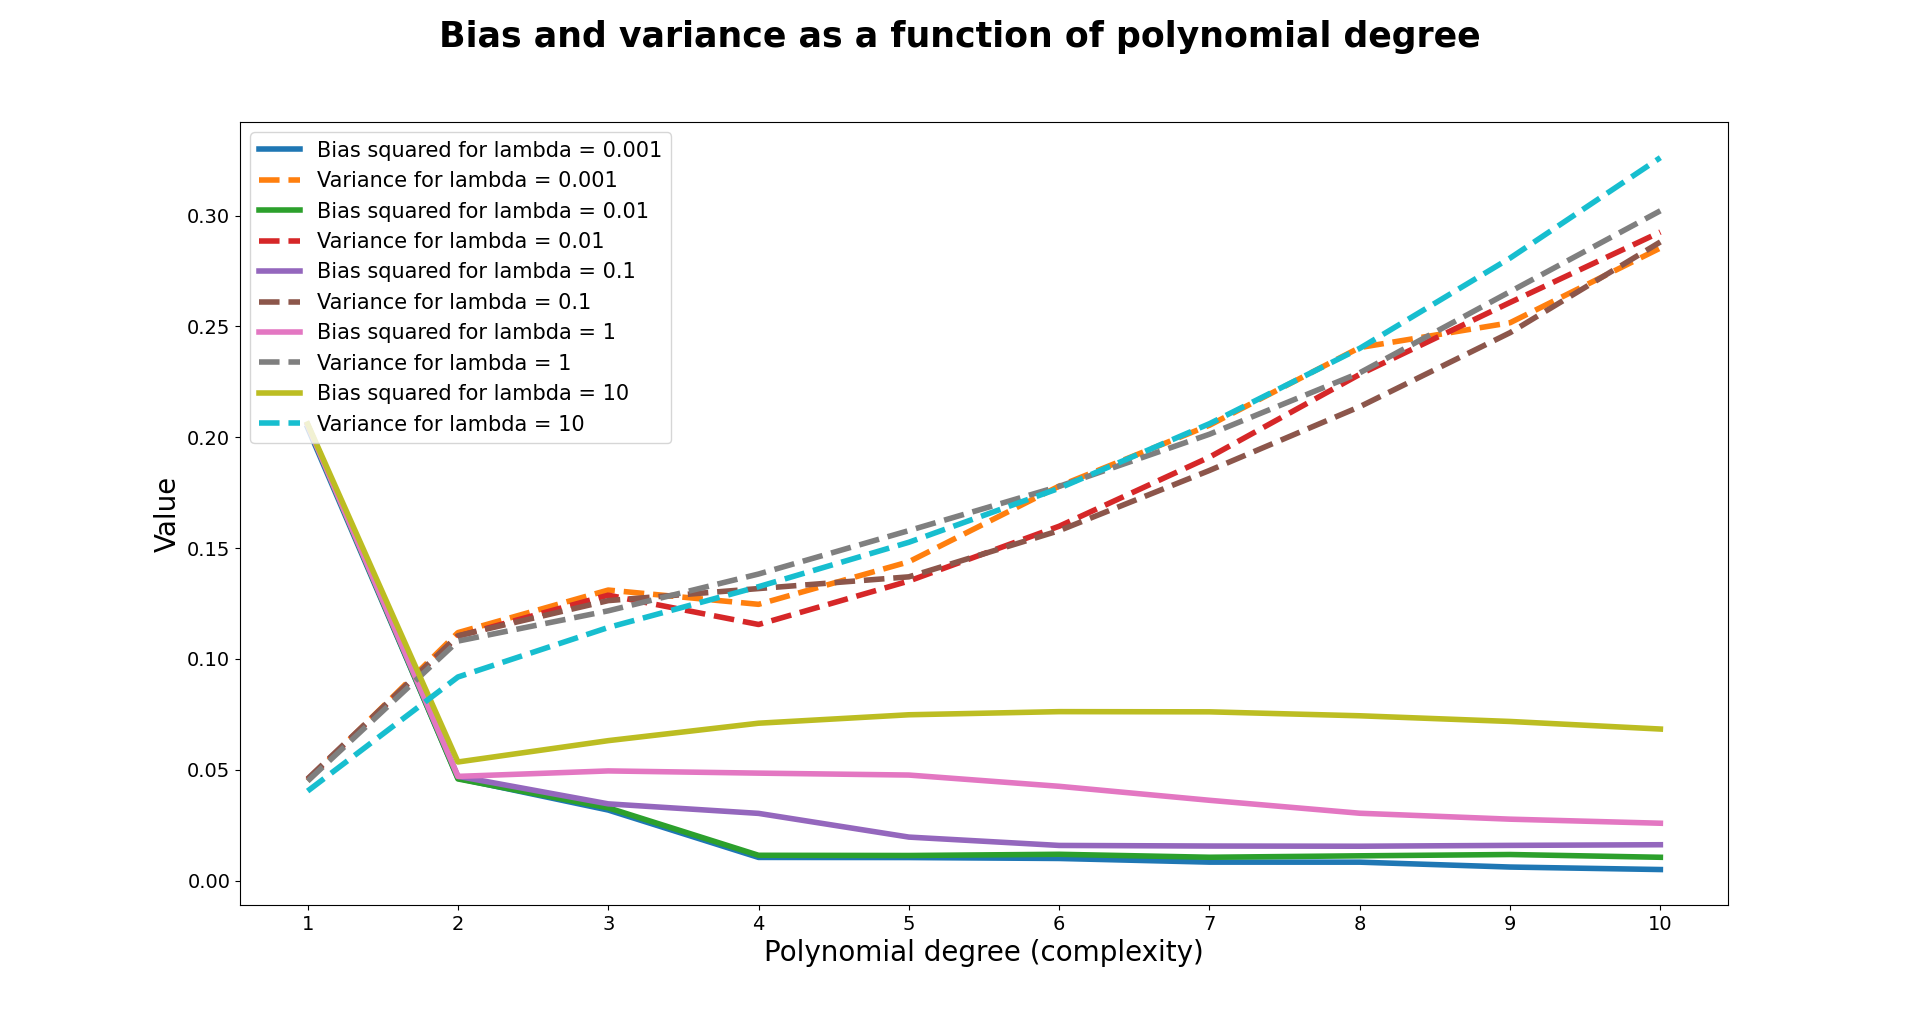
\includegraphics[width = 1\linewidth]{C:/Users/Sander/Documents/GitHub/FYS-STK4155/Project1/Report/Figures/BVplotCV_n100_p10_noise0001_CV10_RIDGE.PNG}
\caption{\label{fig:BVRidgeCV1} Bias and variance decomposition of figure \ref{fig:MSERidgeCV1}. The bias and variance change as a function of polynomial degree and values of $\lambda$ using the 10-fold CV resampling method. Here we have 100 observations with a noise level of $0.001$.}
\end{figure}

\begin{figure}[H]
\centering
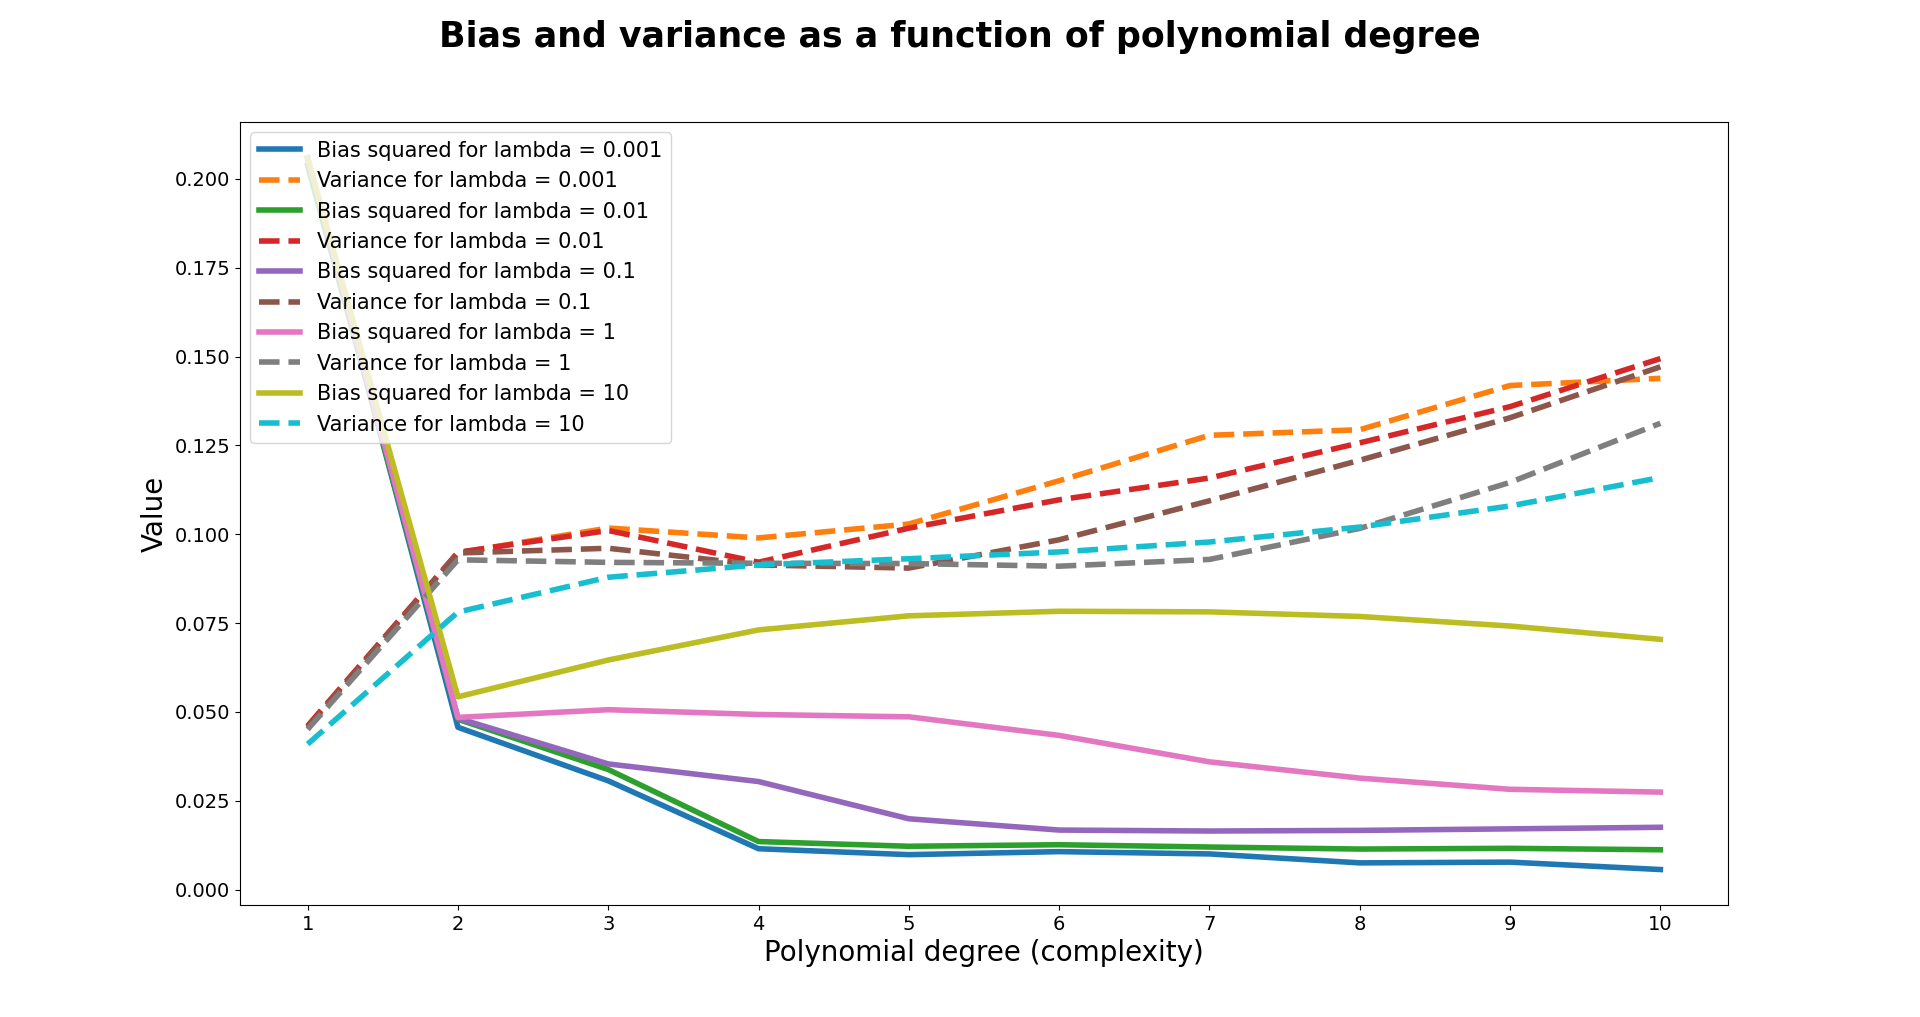
\includegraphics[width = 1\linewidth]{C:/Users/Sander/Documents/GitHub/FYS-STK4155/Project1/Report/Figures/BVplotCV_n100_p10_noise0001_CV5_RIDGE.PNG}
\caption{\label{fig:BVRidgeCV2} Bias and variance decomposition of figure \ref{fig:MSERidgeCV2}. The bias and variance change as a function of polynomial degree and values of $\lambda$ using the 5-fold CV resampling method. Here we have 100 observations with a noise level of $0.001$.}
\end{figure}

\begin{figure}[H]
\centering
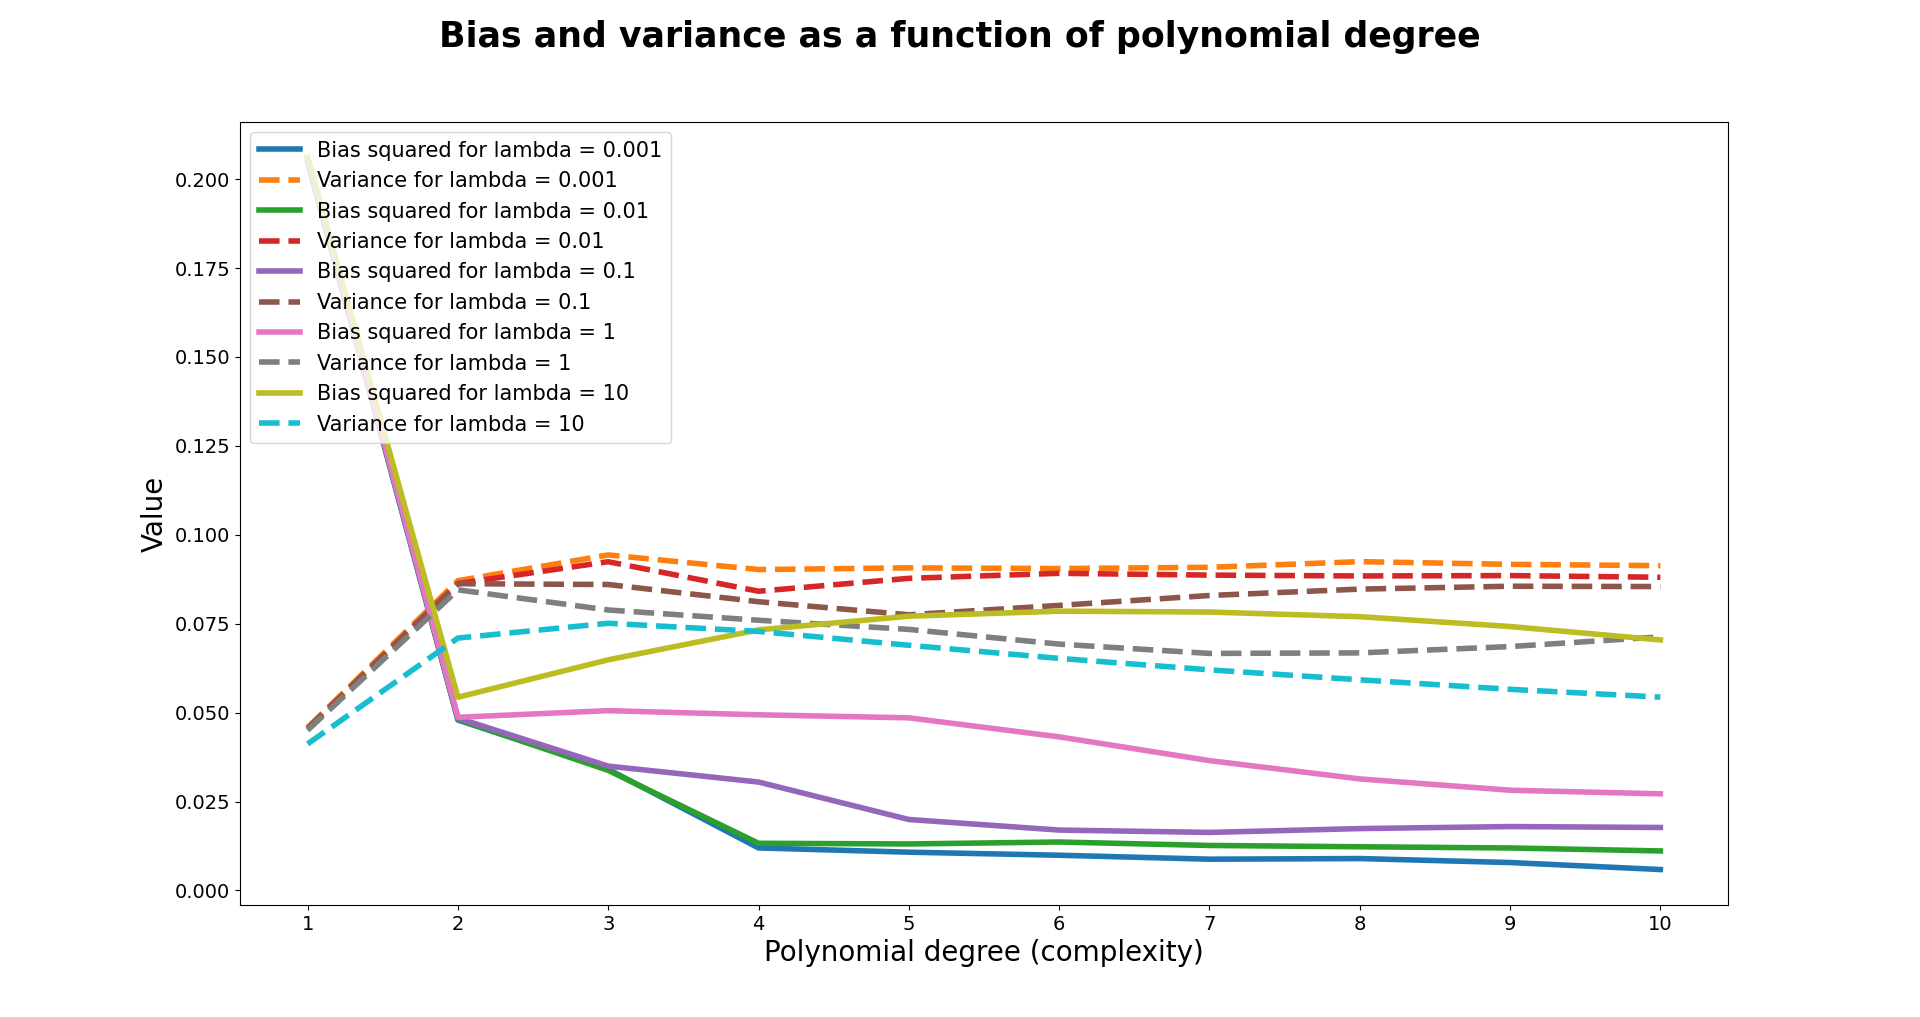
\includegraphics[width = 1\linewidth]{C:/Users/Sander/Documents/GitHub/FYS-STK4155/Project1/Report/Figures/BVplotCV_n100_p10_noise0001_CV1_RIDGE.PNG}
\caption{\label{fig:BVRidgeCV3} Bias and variance decomposition of figure \ref{fig:MSERidgeCV3}. The bias and variance change as a function of polynomial degree and values of $\lambda$ using the LOOCV resampling method. Here we have 100 observations with a noise level of $0.001$.}
\end{figure}

\noindent Figures \ref{fig:BVRidgeCV1}, \ref{fig:BVRidgeCV2} and \ref{fig:BVRidgeCV3} explains why the test MSEs decreased with smaller folds. The bias of stays the same regardless of fold-size, while the variance increases with increasing fold size. We again observe that the LOOCV models never really increase their variance past a certain point. 

\begin{center}
\large{\textbf{Regression coefficients as function of $\lambda$ using cross-validation}}
\end{center}

\noindent Let us now investigate the effects of the Ridge regression on the regression coefficients when we utilize the CV resampling method. We can again plot the regression coefficient values against values of $\lambda$ for all three fold sizes as done in figure \ref{fig:LambdaPlotCV1}, \ref{fig:LambdaPlotCV2} and \ref{fig:LambdaPlotCV3}

\begin{figure}[H]
\centering
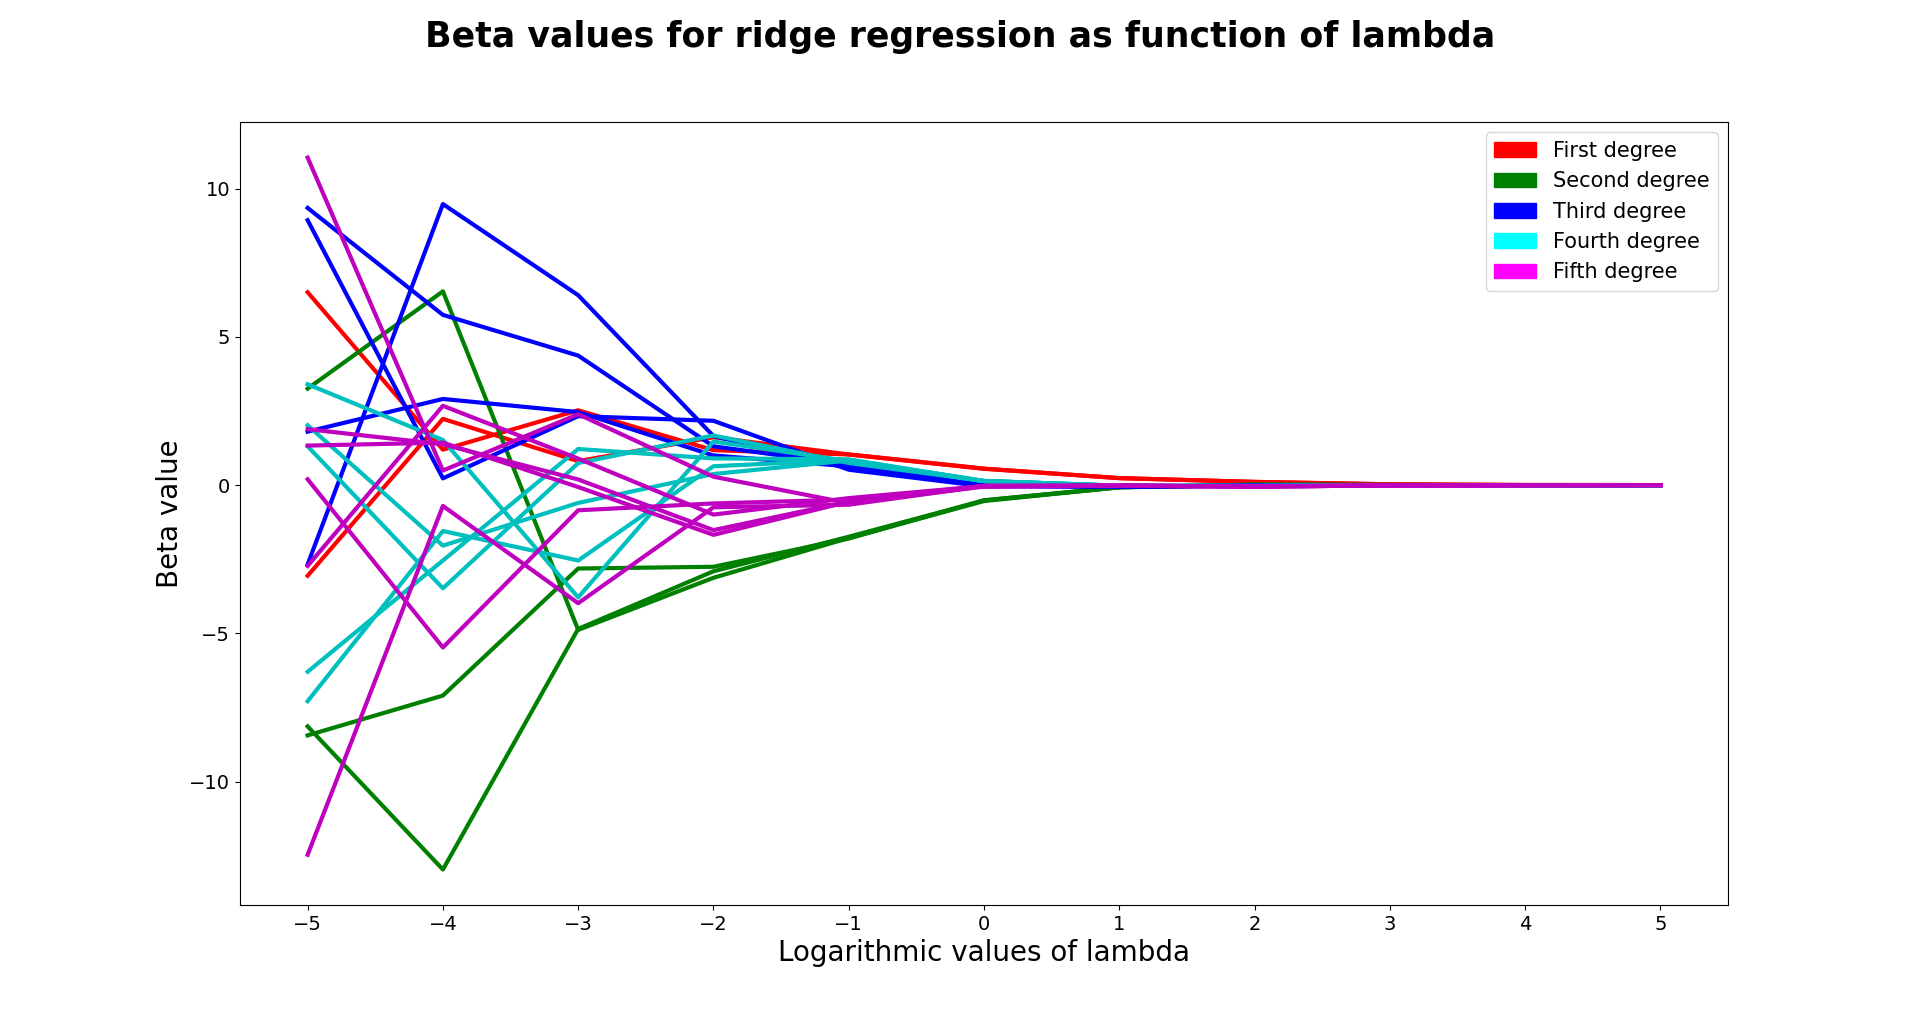
\includegraphics[width = 1\linewidth]{C:/Users/Sander/Documents/GitHub/FYS-STK4155/Project1/Report/Figures/LambdaPlot_n100_p5_noise0001_CV10_RIDGE.PNG}
\caption{\label{fig:LambdaPlotCV1} Regression coefficient values of up to $p = 5$ as function of logarithmic $\lambda$-value using the 10-fold CV method. The original dataset is of size 100. Here we have sorted polynomials of the same degree into the same color.}
\end{figure}

\begin{figure}[H]
\centering
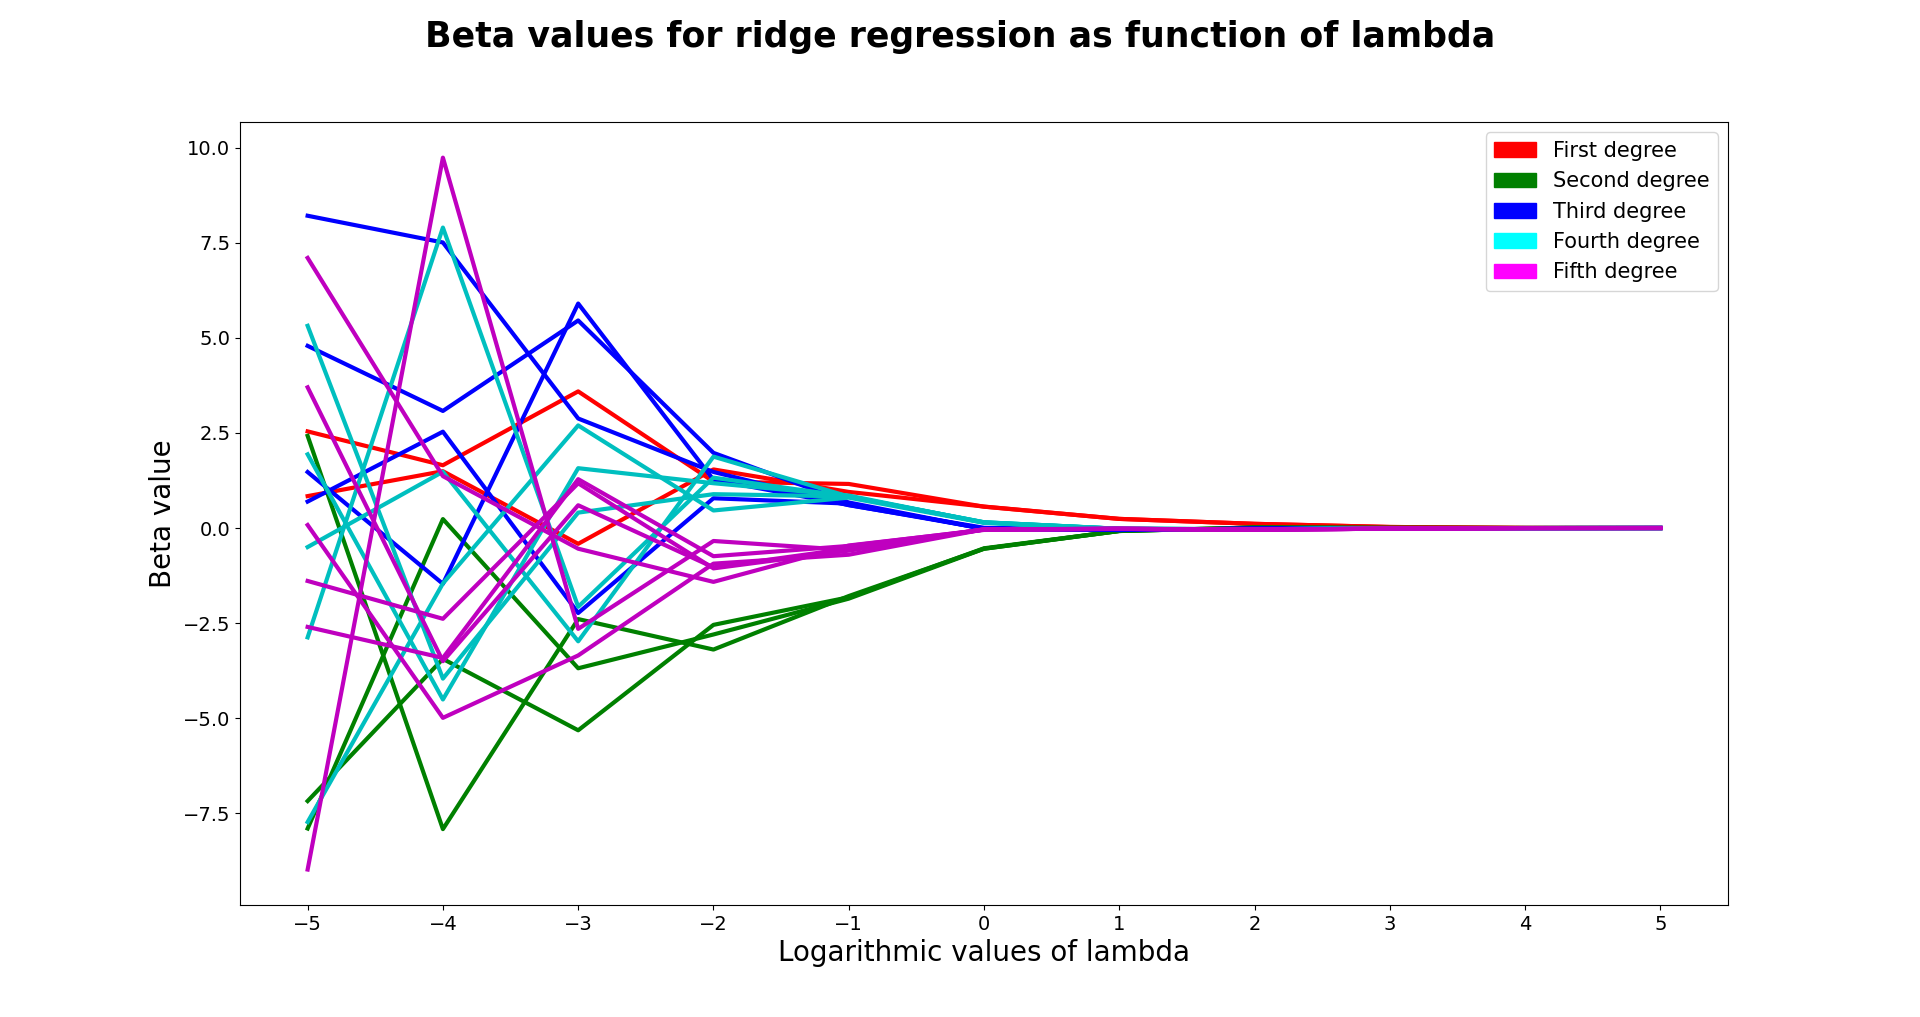
\includegraphics[width = 1\linewidth]{C:/Users/Sander/Documents/GitHub/FYS-STK4155/Project1/Report/Figures/LambdaPlot_n100_p5_noise0001_CV5_RIDGE.PNG}
\caption{\label{fig:LambdaPlotCV2} Regression coefficient values of up to $p = 5$ as function of logarithmic $\lambda$-value using the 5-fold CV method. The original dataset is of size 100. Here we have sorted polynomials of the same degree into the same color.}
\end{figure}

\begin{figure}[H]
\centering
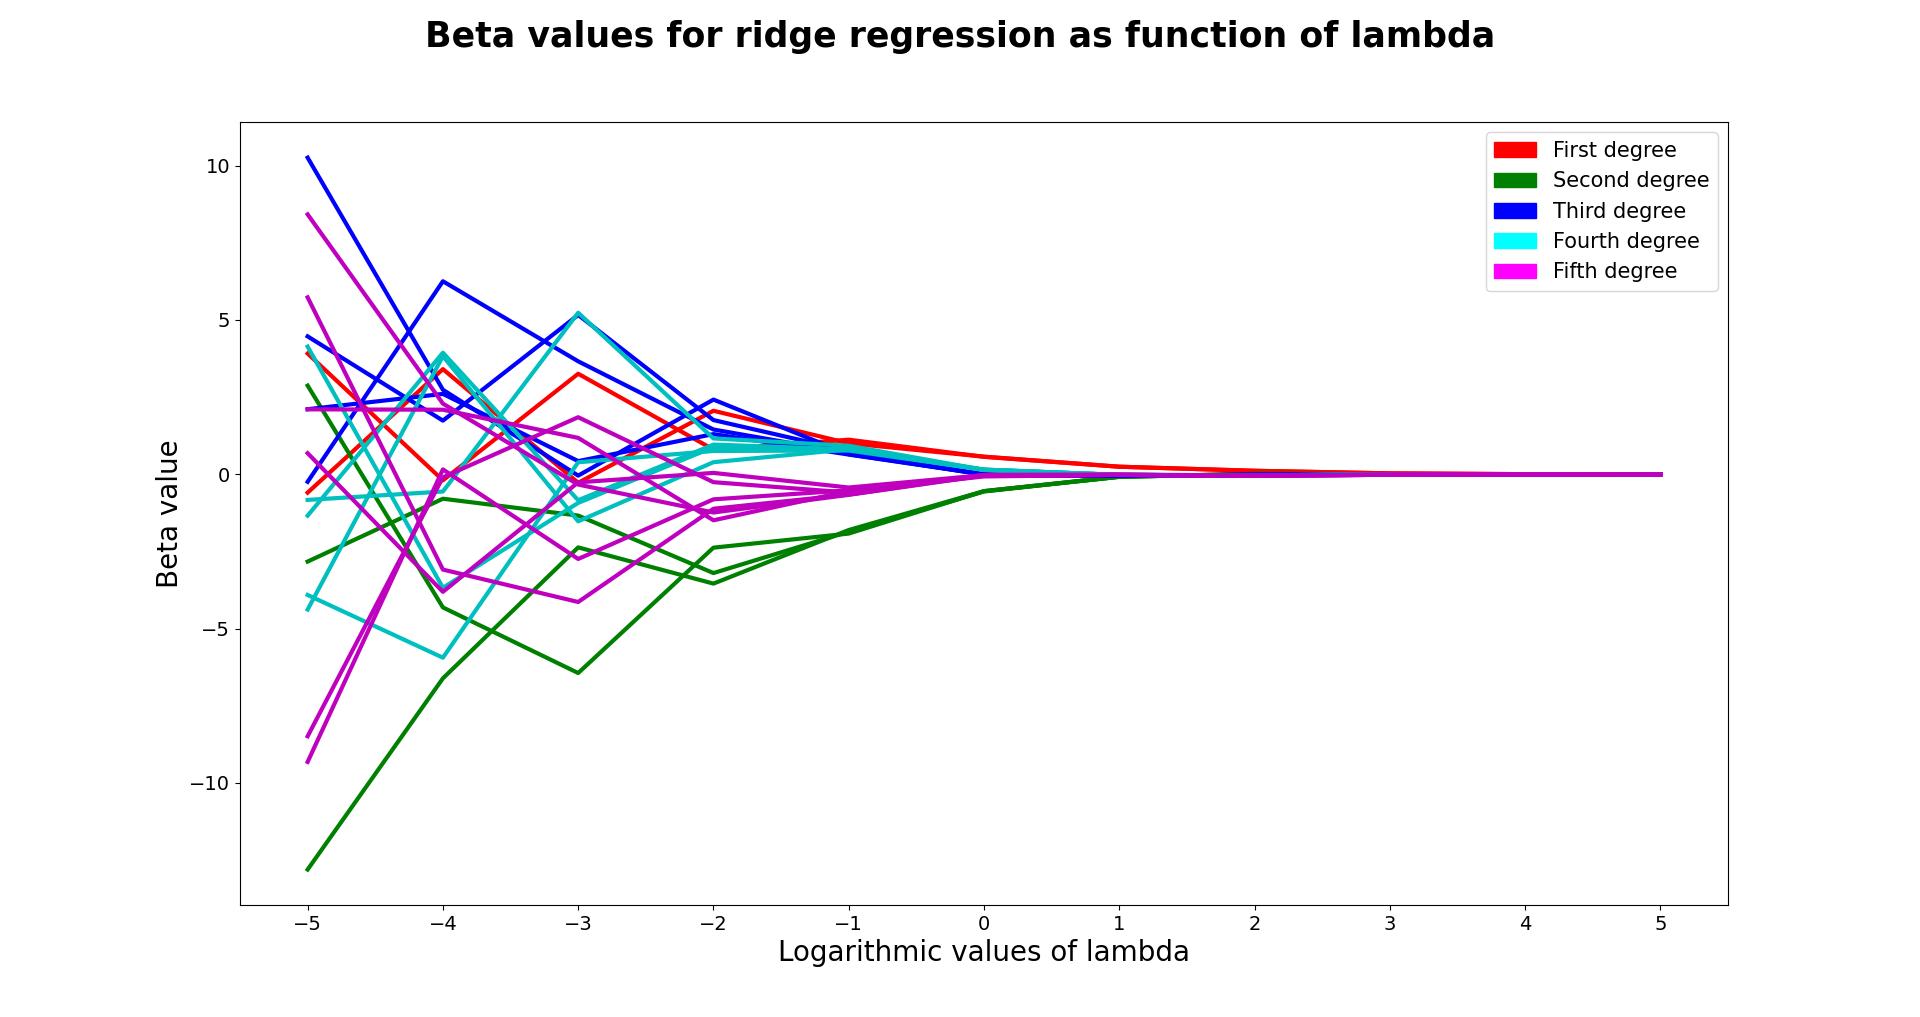
\includegraphics[width = 1\linewidth]{C:/Users/Sander/Documents/GitHub/FYS-STK4155/Project1/Report/Figures/LambdaPlot_n100_p5_noise0001_CV1_RIDGE.PNG}
\caption{\label{fig:LambdaPlotCV3} Regression coefficient values of up to $p = 5$ as function of logarithmic $\lambda$-value using the LOOCV method. The original dataset is of size 100. Here we have sorted polynomials of the same degree into the same color}
\end{figure}

\noindent One can observe that the regression coefficients all approach zero at about the same rate for all fold sizes. If we compared figures \ref{fig:LambdaPlotCV1}, \ref{fig:LambdaPlotCV2} and \ref{fig:LambdaPlotCV3} to figures \ref{fig:LambdaPlot2}, we observe that the regression coefficient values are higher for the CV resampling method. However, this is meaningless as it is when the coefficients approach zero that matters. With that, we again compare the figures and see that the Ridge regression reduces variables towards zero quicker when we use the CV resampling method, rather than the bootstrap method.
\\
With the information we have gathered so far, we can safely say that the Ridge regression has a larger impact when we utilize the CV resampling method more than the bootstrap resampling method.

\newpage

\begin{center}
\Large{\textbf{Exercise 1e) Lasso regression}}
\end{center}

\begin{center}
\large{\textbf{Lasso regression MSE as function of model complexity using bootstrap}}
\end{center}

\noindent We now investigate the second shrinkage method, namely the Lasso regression. Like the Ridge regression, the Lasso shrinks the least significant variables, but the variables are set to exactly zero and not just close to zero. We can write the Lasso regression equation to be the same as the Ridge regression coefficient equation but with using the L1 norm instead of L2 norm (Hastie, T., et al., 2009, [C])

\begin{equation}\label{eq:LassoDerive2}
\begin{aligned}
\boldsymbol{\hat{\beta}}^{Lasso} = argmin_{\beta}(\frac{1}{2}\sum_{i = 1}^n(y_i - \boldsymbol{\hat{\beta}} - \sum_{j = 1}^p x_{i,j}\boldsymbol{\hat{\beta}}_j)^2 + \lambda \sum_{j = 1}^p |\boldsymbol{\hat{\beta}} |)
\end{aligned}
\end{equation}

\noindent where $\boldsymbol{\hat{\beta}}$ is the ordinary least squares regression coefficients given by equation \ref{eq:minBeta}. We can then perform the exact same investigation as done in exercise d, where we first plot the MSE as function of model complexity and the regression coefficients as function of $\lambda$ for the bootstrap resampling method as well as for 10-fold, 5-fold and leave-one-out cross-validations. However, as the Lasso regression is difficult to implement, the Scikit-Learn functionality will be used. The MSE plots are shown in figures \ref{fig:MSELasso1}, \ref{fig:MSELasso2}, \ref{fig:MSELasso3} and \ref{fig:MSELasso4}

\begin{figure}[H]
\centering
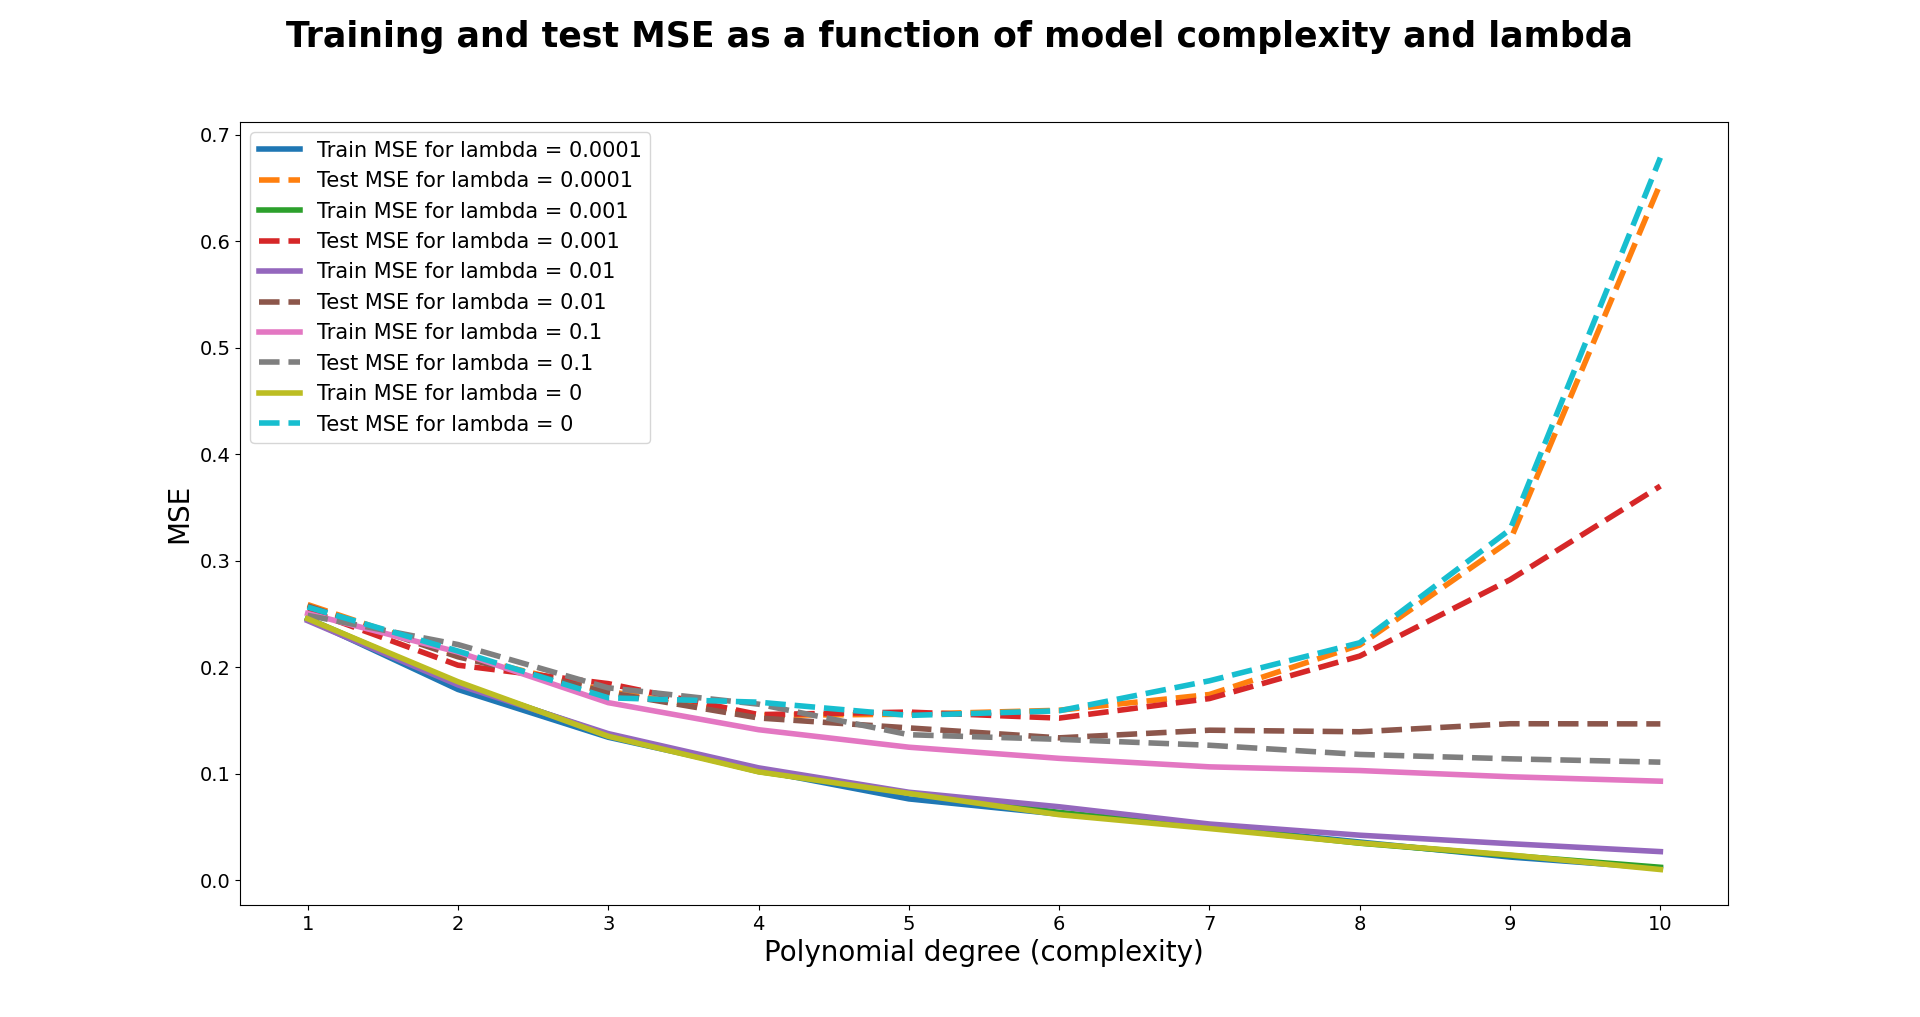
\includegraphics[width = 1\linewidth]{C:/Users/Sander/Documents/GitHub/FYS-STK4155/Project1/Report/Figures/MSEBOOT_n100_p10_noise0001_ts025_B100_Lasso.PNG}
\caption{\label{fig:MSELasso1} MSE as a function of polynomial degree up to 10 for different values of $\lambda$ using the bootstrap resampling method and a Lasso regression scheme. Here we have $100 \times 100$ observations randomly drawn from the original data with a noise level of $0.001$.}
\end{figure}

\begin{figure}[H]
\centering
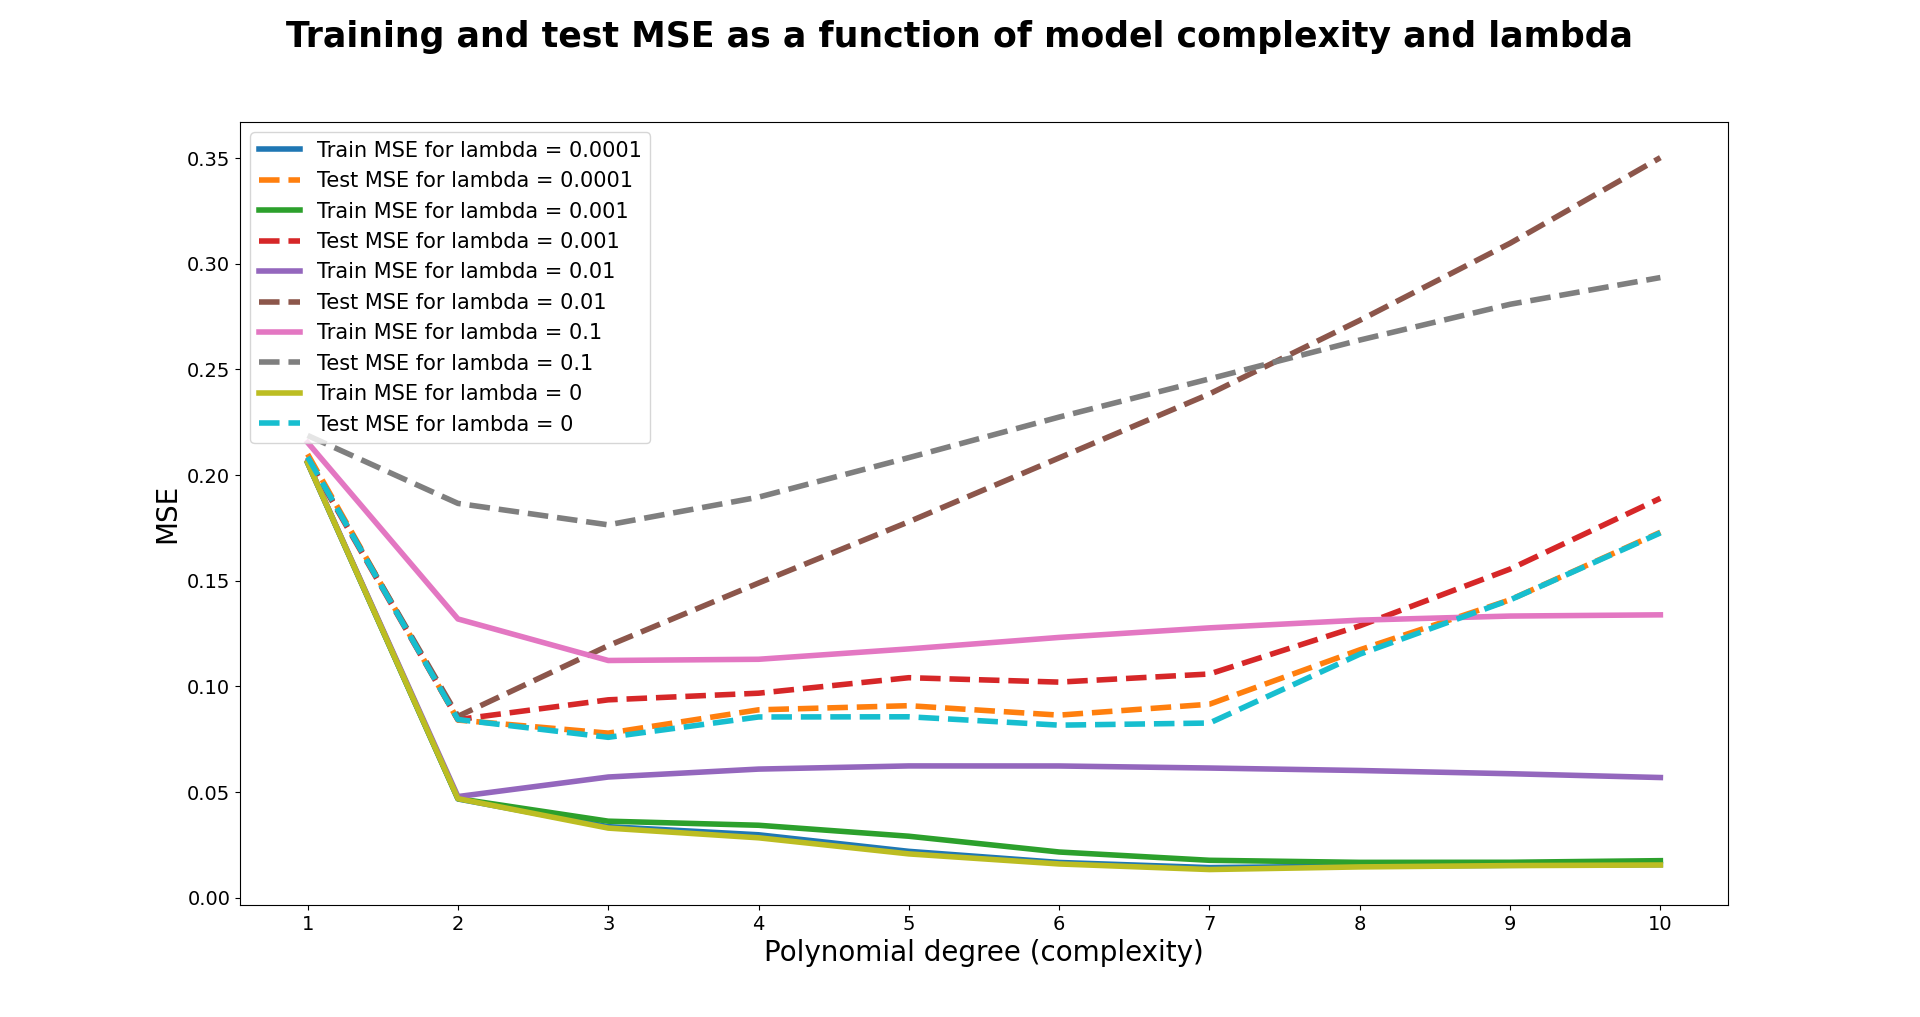
\includegraphics[width = 1\linewidth]{C:/Users/Sander/Documents/GitHub/FYS-STK4155/Project1/Report/Figures/MSECV_n100_p10_noise0001_CV10_Lasso.PNG}
\caption{\label{fig:MSELasso2} MSE as a function of polynomial degree up to 10 for different values of $\lambda$ using the 10-fold CV resampling method and a Lasso regression scheme. Here we have 100 observations while we consider every possible permutation of a 10-fold cross-validation with a noise level of $0.001$.}
\end{figure}

\begin{figure}[H]
\centering
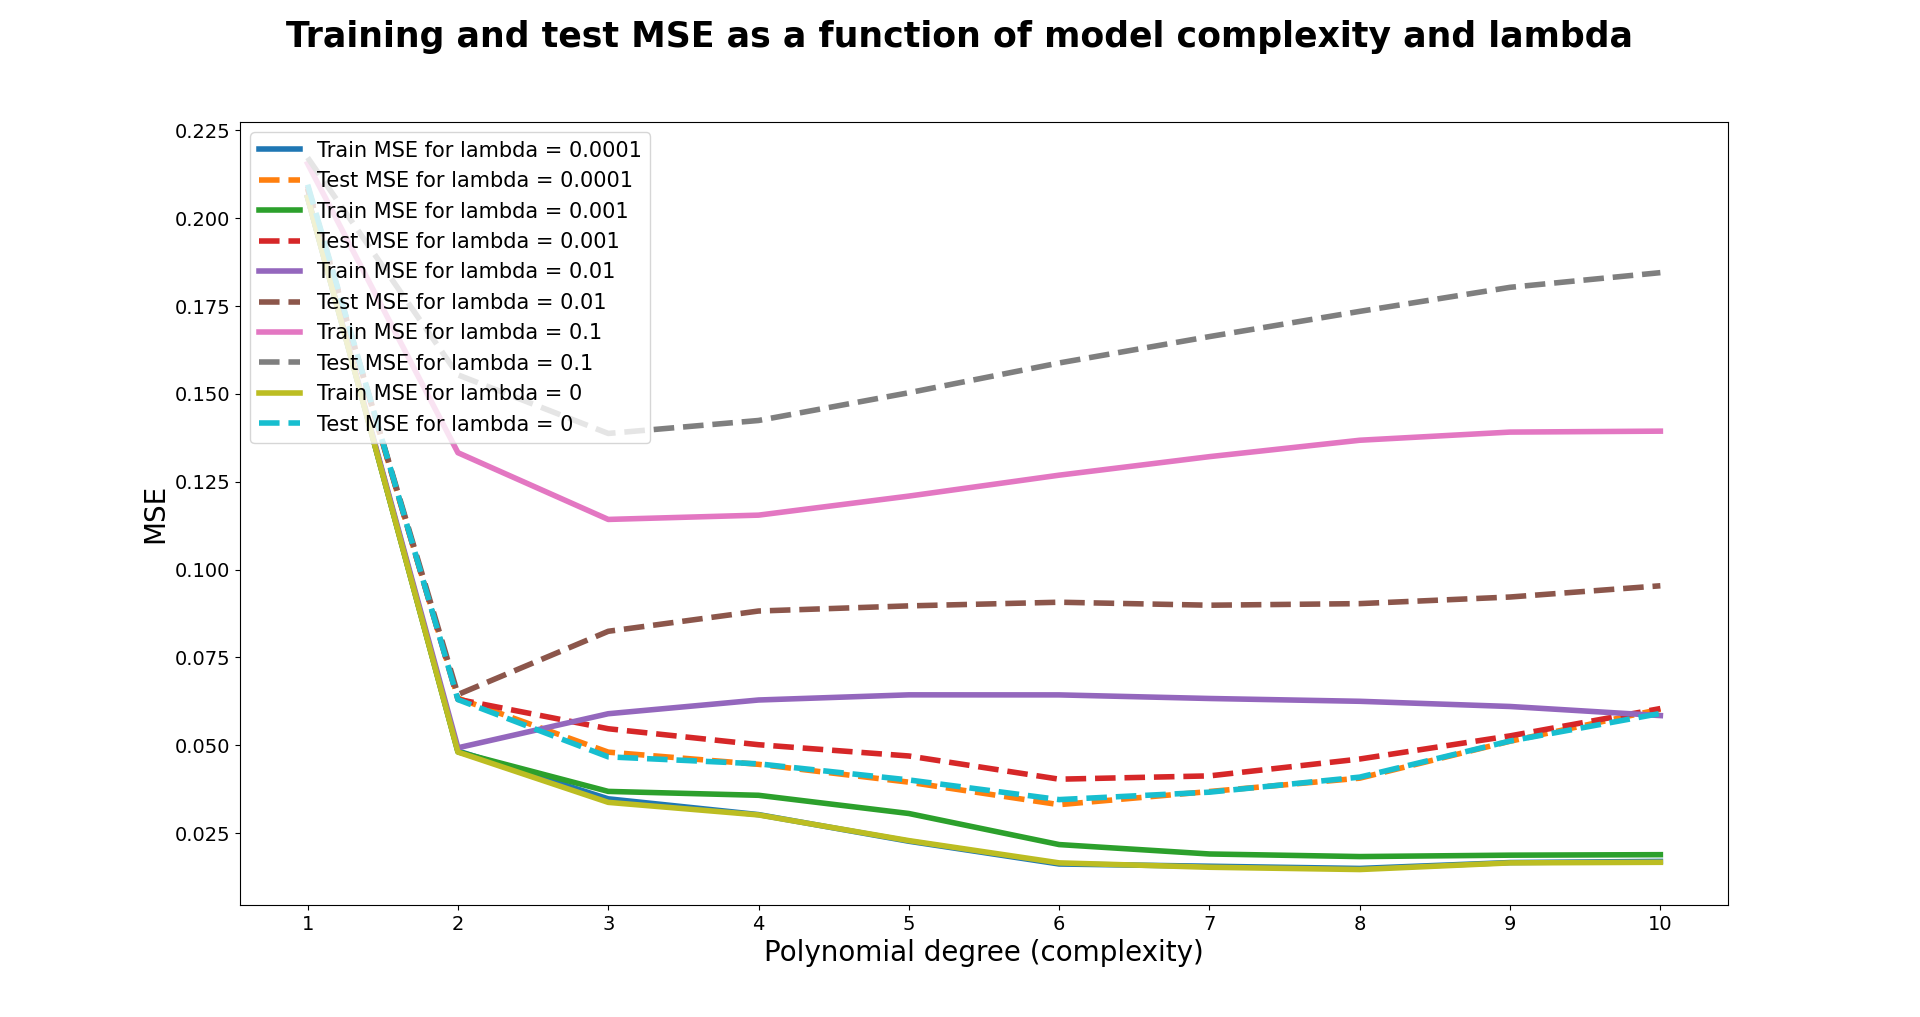
\includegraphics[width = 1\linewidth]{C:/Users/Sander/Documents/GitHub/FYS-STK4155/Project1/Report/Figures/MSECV_n100_p10_noise0001_CV5_Lasso.PNG}
\caption{\label{fig:MSELasso3} MSE as a function of polynomial degree up to 10 for different values of $\lambda$ using the 5-fold CV resampling method and a Lasso regression scheme. Here we have 100 observations while we consider every possible permutation of a 5-fold cross-validation with a noise level of $0.001$.}
\end{figure}

\begin{figure}[H]
\centering
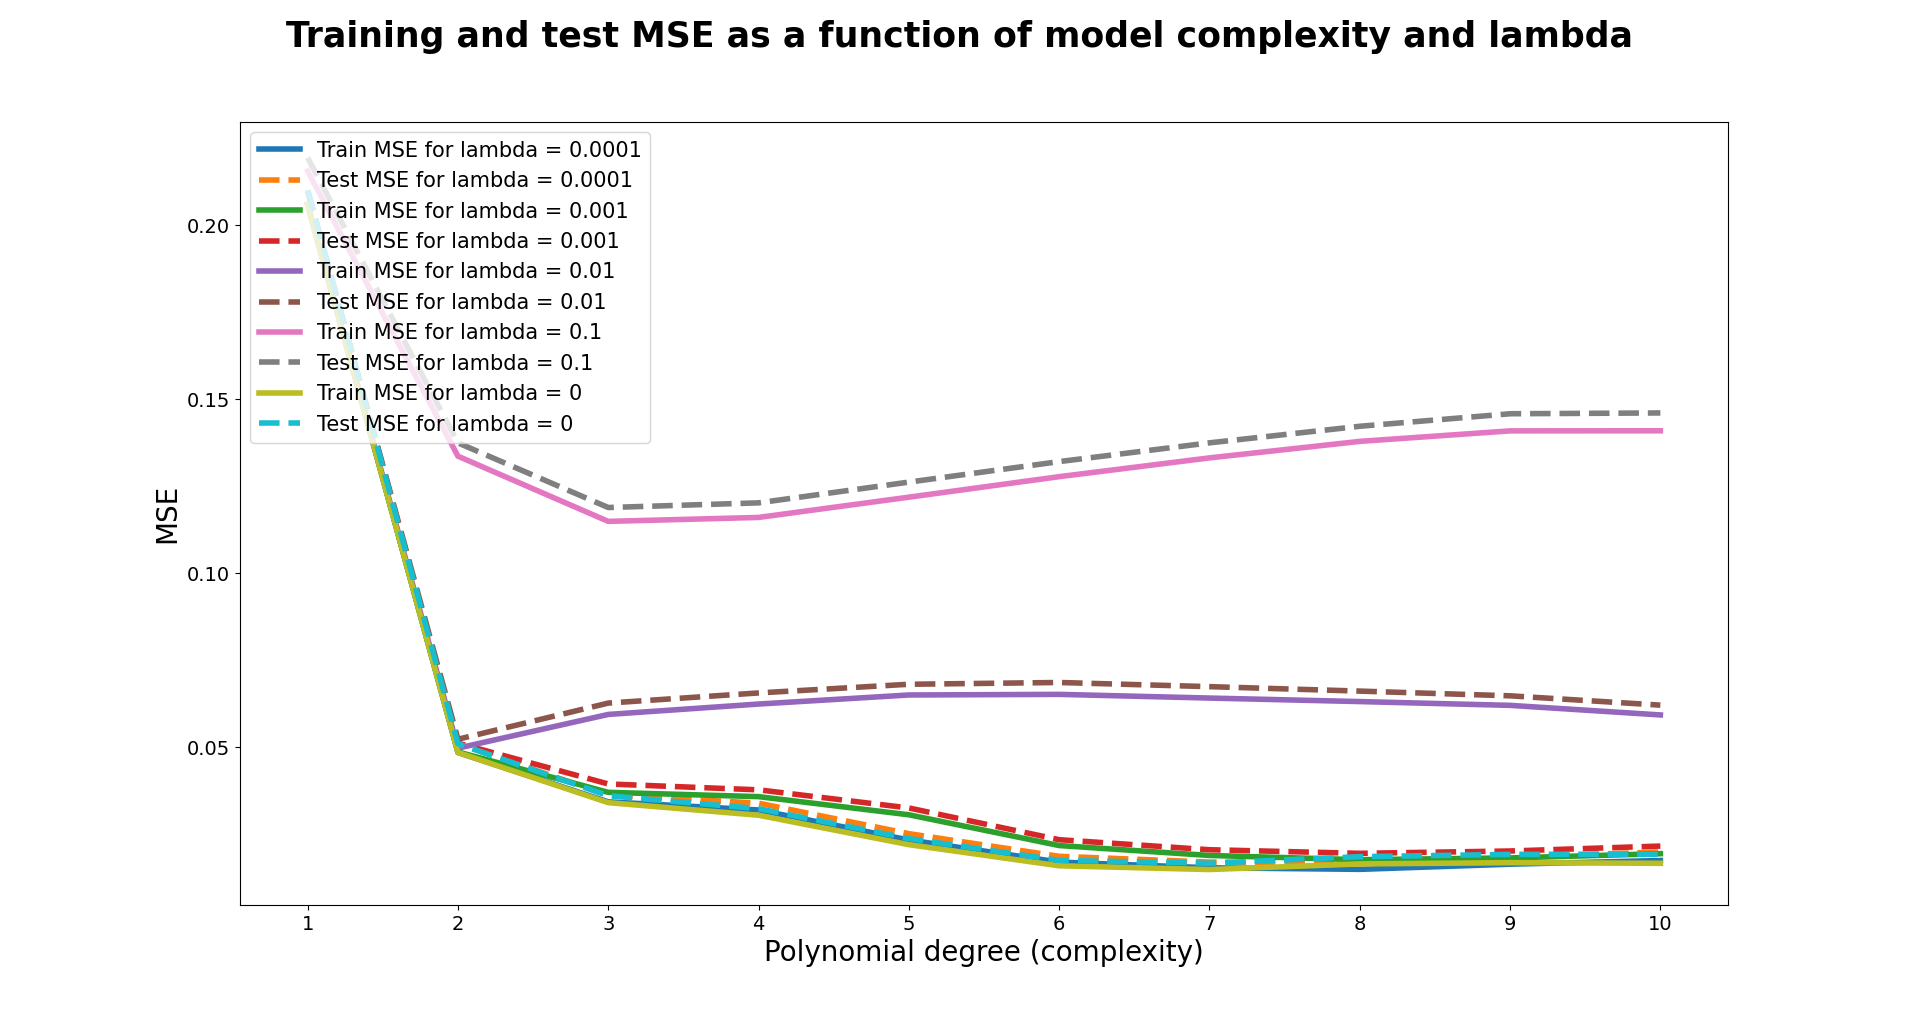
\includegraphics[width = 1\linewidth]{C:/Users/Sander/Documents/GitHub/FYS-STK4155/Project1/Report/Figures/MSECV_n100_p10_noise0001_CV1_Lasso.PNG}
\caption{\label{fig:MSELasso4} MSE as a function of polynomial degree up to 10 for different values of $\lambda$ using the LOOCV resampling method and a Lasso regression scheme. Here we have 100 observations while we consider every possible permutation of a LOOCV with a noise level of $0.001$.}
\end{figure}

\noindent Let us first discuss the difference between the bootstrap resampling method seen in figure \ref{fig:MSELasso1} and the CV resampling method seen in figures \ref{fig:MSELasso2}, \ref{fig:MSELasso3} and \ref{fig:MSELasso4}. The models creating using bootstrap seem much smoother than the models using CV. More importantly, we observe that the bootstrap models tend to increase their MSE exponentially, while the CV models tend to increase their MSE linearly. This may be important if one wishes to create a model of a high degree without letting the MSE get out of hand. Additionally, the CV models have lower overall test MSE than the bootstrap equivalent. 
\\
As for the dependence on different $\lambda$-values, we can observe that lower $\lambda$-values tend to lie close to the OLS model ($\lambda = 0$). However, when $\lambda$ is increased in the bootstrap method, the overall test MSE decreases while the opposite is the case in the CV method. 
\\
Another observations is that some models using low values of $\lambda$ never really increase in MSE. This is particularly the case for the bootstrap and LOOCV models where polynomials of degree 10 have less $0.1$ in MSE. Such a feet is possible due to the variable shrinkage done by the Lasso regression scheme. Removing variables makes the model less prone to over-fitting, thus reducing the MSE at higher complexity. This means that using models with a high number of bootstrap iterations or low number of folds while using low values of $\lambda$ allows us to create a model for higher order polynomials, which in turn may increase the models predictive capabilities.
\\
Let us now study how the regression coefficients change as a function of $\lambda$ as we already suspect that some of them have been set to zero by the Lasso regression scheme. Figure \ref{fig:LambdaLasso1}, \ref{fig:LambdaLasso2}, \ref{fig:LambdaLasso3} and \ref{fig:LambdaLasso4} show how regression coefficients behave as function of $\lambda$

\begin{figure}[H]
\centering
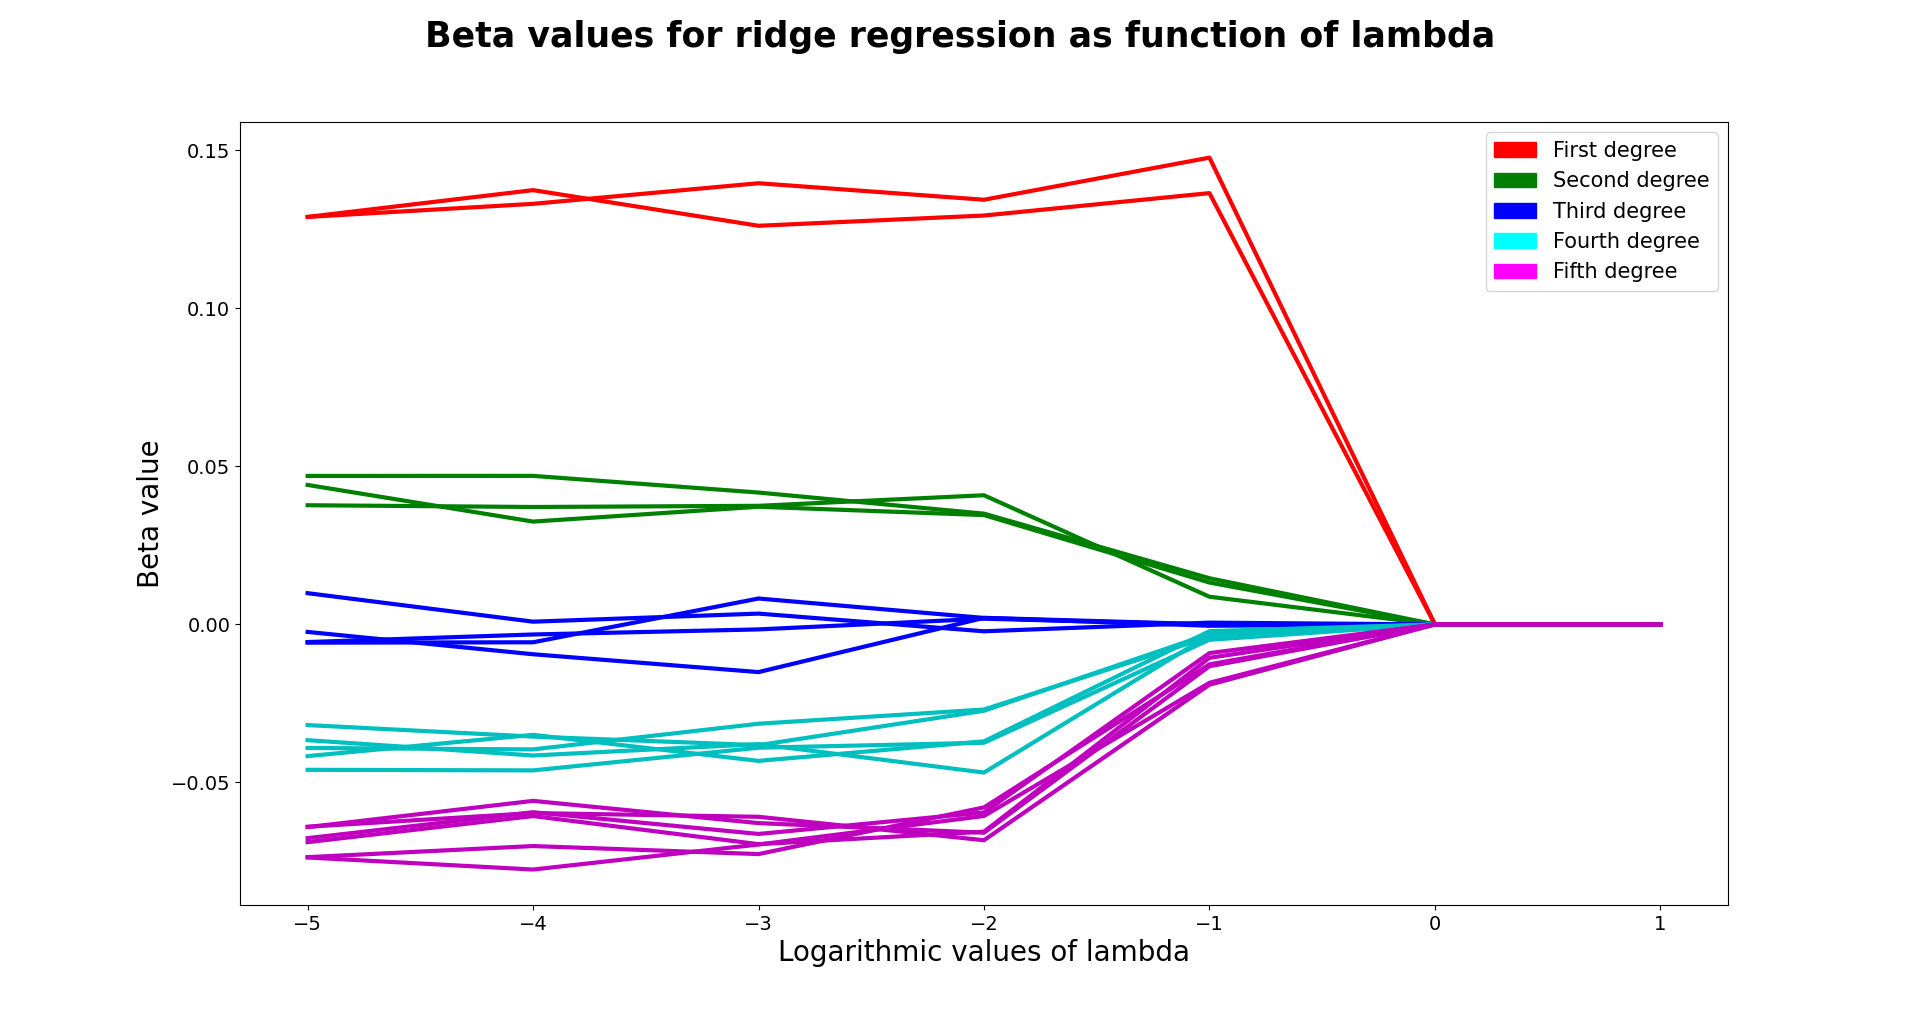
\includegraphics[width = 1\linewidth]{C:/Users/Sander/Documents/GitHub/FYS-STK4155/Project1/Report/Figures/LambdaPlot_n100_p5_noise0001_ts025_B100_LassoSort.PNG}
\caption{\label{fig:LambdaLasso1} Regression coefficient values of up to $p = 5$ as function of logarithmic $\lambda$-value using the bootstrap resampling method. The original dataset is of size 100 with a noise-level of $0.001$. Here we have sorted polynomials of the same degree into the same color.}
\end{figure}

\begin{figure}[H]
\centering
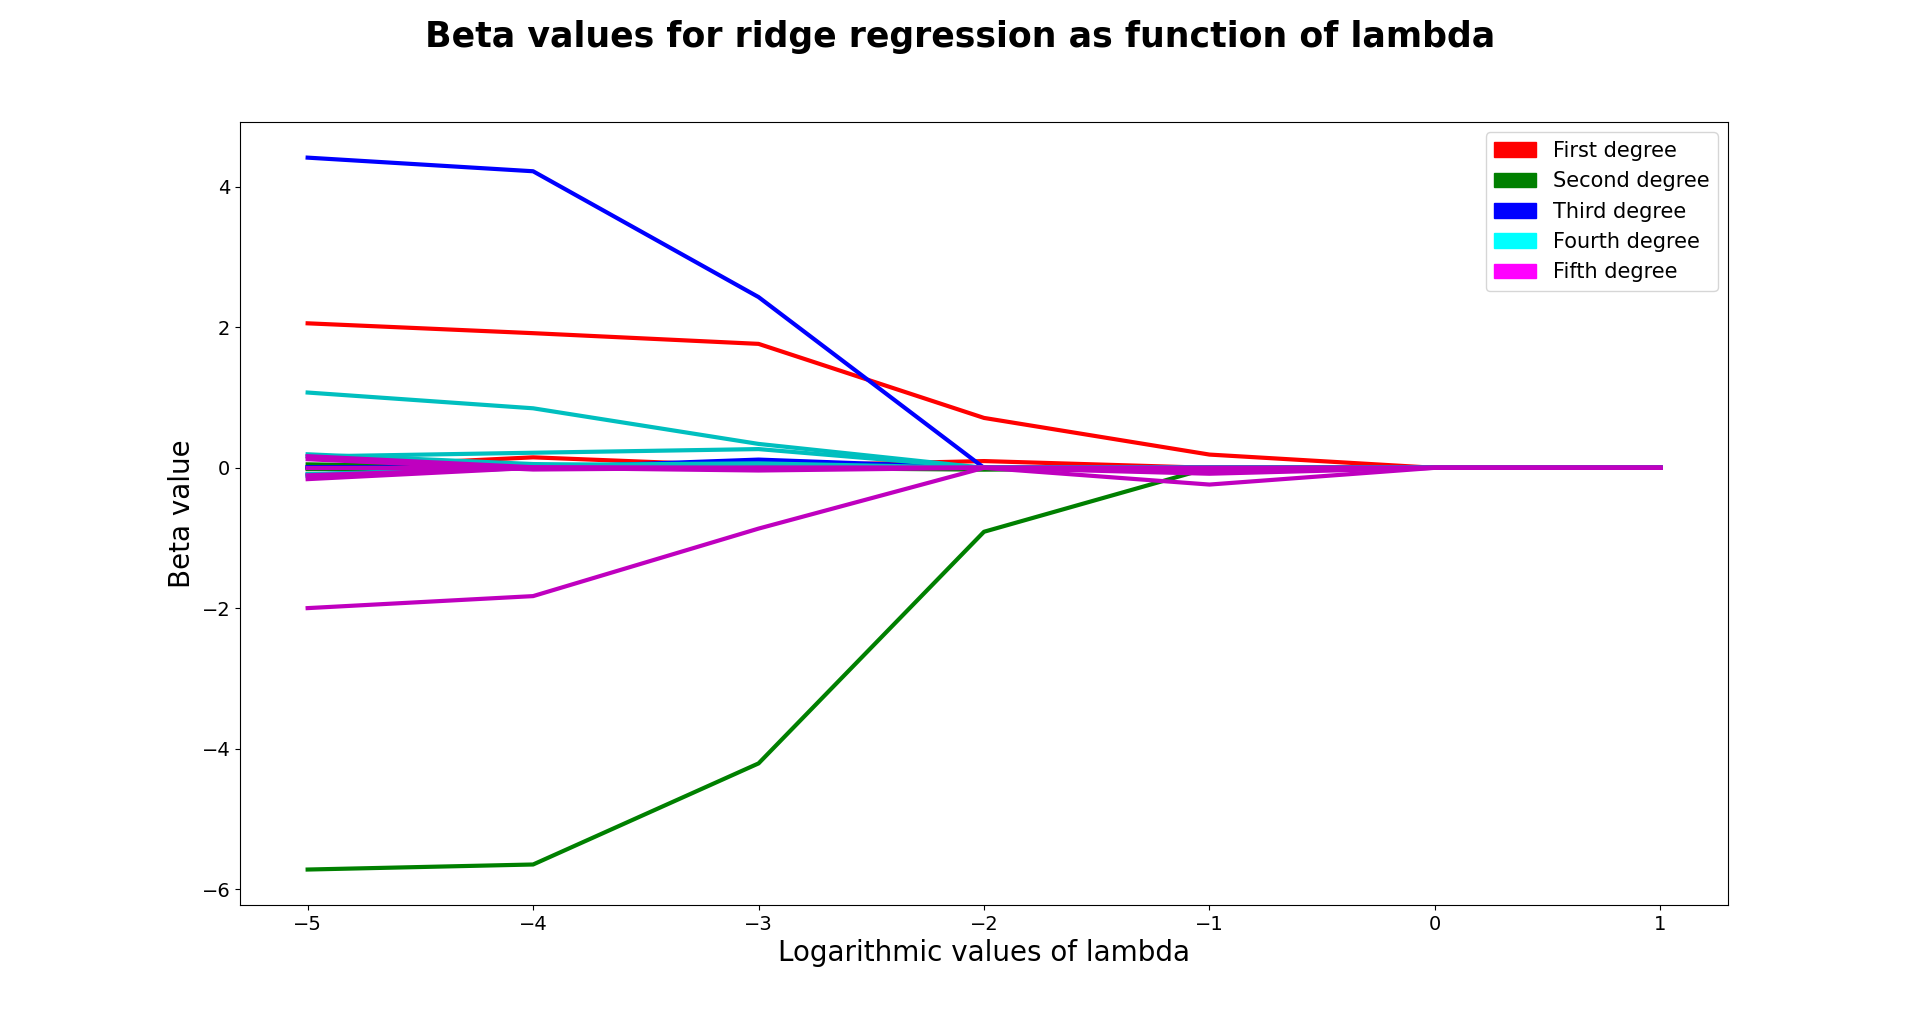
\includegraphics[width = 1\linewidth]{C:/Users/Sander/Documents/GitHub/FYS-STK4155/Project1/Report/Figures/LambdaPlot_n100_p5_noise0001_CV10_LassoSort.PNG}
\caption{\label{fig:LambdaLasso2} Regression coefficient values of up to $p = 5$ as function of logarithmic $\lambda$-value using the 10-fold CV resampling method. The original dataset is of size 100 with a noise-level of $0.001$. Here we have sorted polynomials of the same degree into the same color.}
\end{figure}

\begin{figure}[H]
\centering
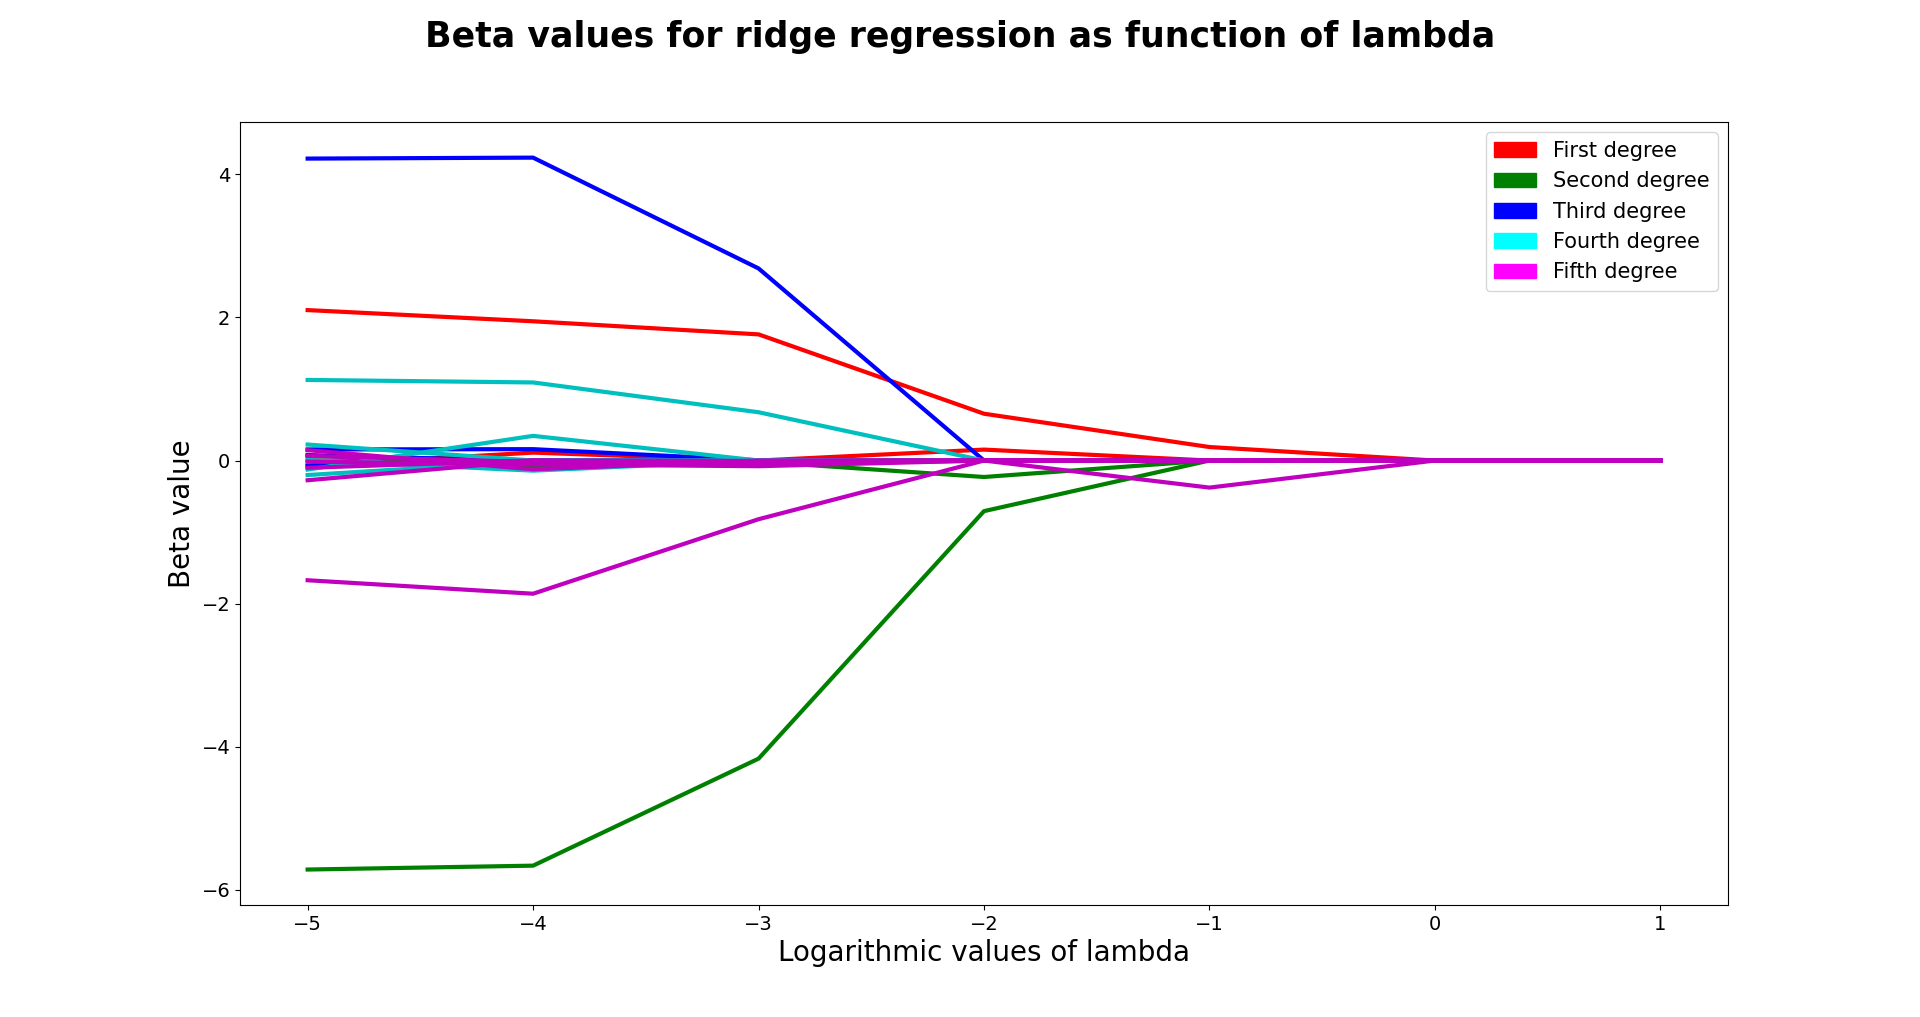
\includegraphics[width = 1\linewidth]{C:/Users/Sander/Documents/GitHub/FYS-STK4155/Project1/Report/Figures/LambdaPlot_n100_p5_noise0001_CV5_LassoSort.PNG}
\caption{\label{fig:LambdaLasso3} Regression coefficient values of up to $p = 5$ as function of logarithmic $\lambda$-value using the 5-fold CV resampling method. The original dataset is of size 100 with a noise-level of $0.001$. Here we have sorted polynomials of the same degree into the same color.}
\end{figure}

\begin{figure}[H]
\centering
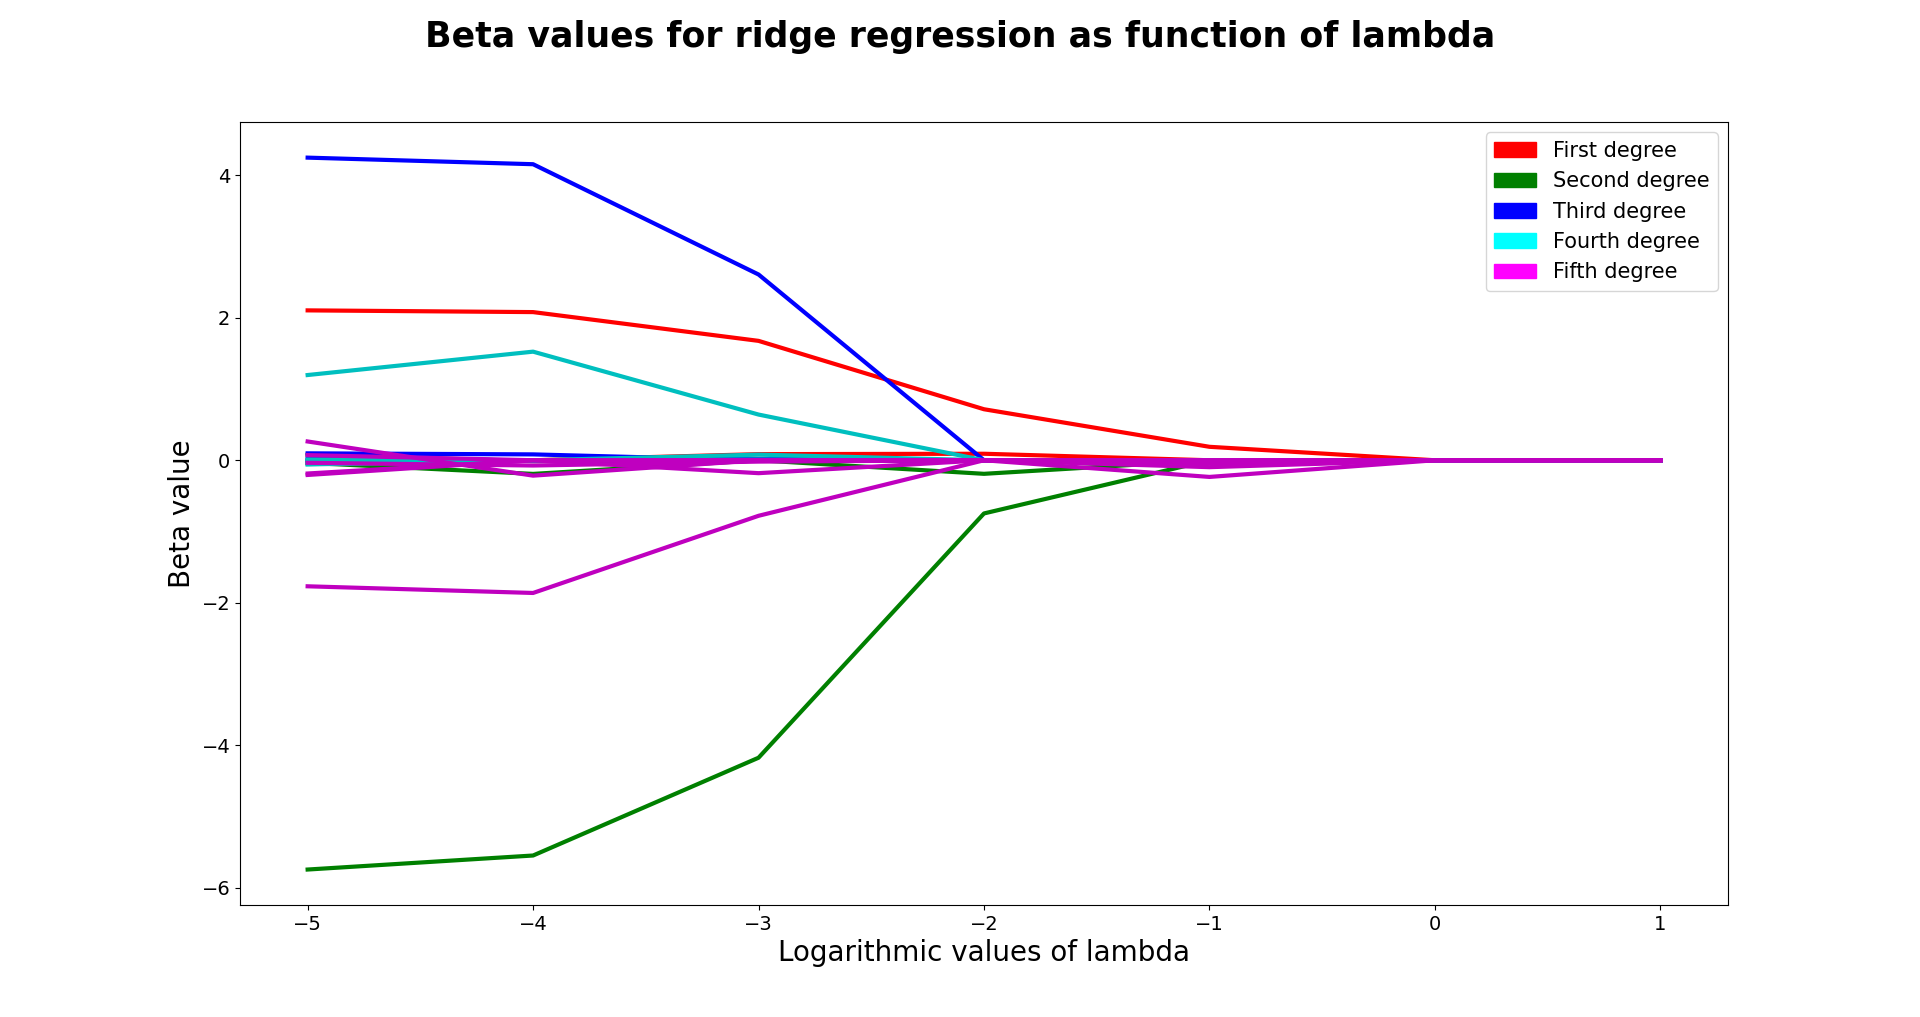
\includegraphics[width = 1\linewidth]{C:/Users/Sander/Documents/GitHub/FYS-STK4155/Project1/Report/Figures/LambdaPlot_n100_p5_noise0001_CV1_LassoSort.PNG}
\caption{\label{fig:LambdaLasso4} Regression coefficient values of up to $p = 5$ as function of logarithmic $\lambda$-value using the LOOCV resampling method. The original dataset is of size 100 with a noise-level of $0.001$. Here we have sorted polynomials of the same degree into the same color.}
\end{figure}

\noindent Comparing the above plots really shows the difference in how the bootstrap and CV resampling methods behave with respect to their models regression coefficients. We can observe that both methods shrink the variables to zero, but at different values of $\lambda$. The CV methods (which all seem to be equivalent) reduce some variables to zero very quickly, particularly the higher order polynomials, while others remain non-zero for longer, namely the lower order polynomials. This is contrary to the bootstrap method where variables tend to be reduced to zero at about the same value of $\lambda$ (except third degree polynomials). This may explain why the OLS is the model with the lowest MSE when we use CV rather than bootstrap. It may be that the variables are set to zero to early making the model unable to accurately predict the Franke function.
\\
We also notice that the Lasso regression reduces the variables at lower values of $\lambda$ than the Ridge regression (figures \ref{fig:LambdaPlot2}, \ref{fig:LambdaPlotCV1}, \ref{fig:LambdaPlotCV2} and \ref{fig:LambdaPlotCV3}). 

\newpage

\begin{center}
\Large{\textbf{Exercise 1f) Preparing real data}}
\end{center}

\begin{center}
\large{\textbf{Data preparation}}
\end{center}

\noindent In this exercise we prepare the terrain data set called "SRTM\textunderscore data\textunderscore Norway\textunderscore 1" which is data collected from Norway. This data was chosen as there was trouble registering an account on the webpage \href{{https://earthexplorer.usgs.gov/}}{\nolinkurl{https://earthexplorer.usgs.gov/}} where the data is taken from, so I settled for the given data set on the FYS-STK4155 github page. The terrain data is loaded into python and the following image is obtained

\begin{figure}[H]
\centering
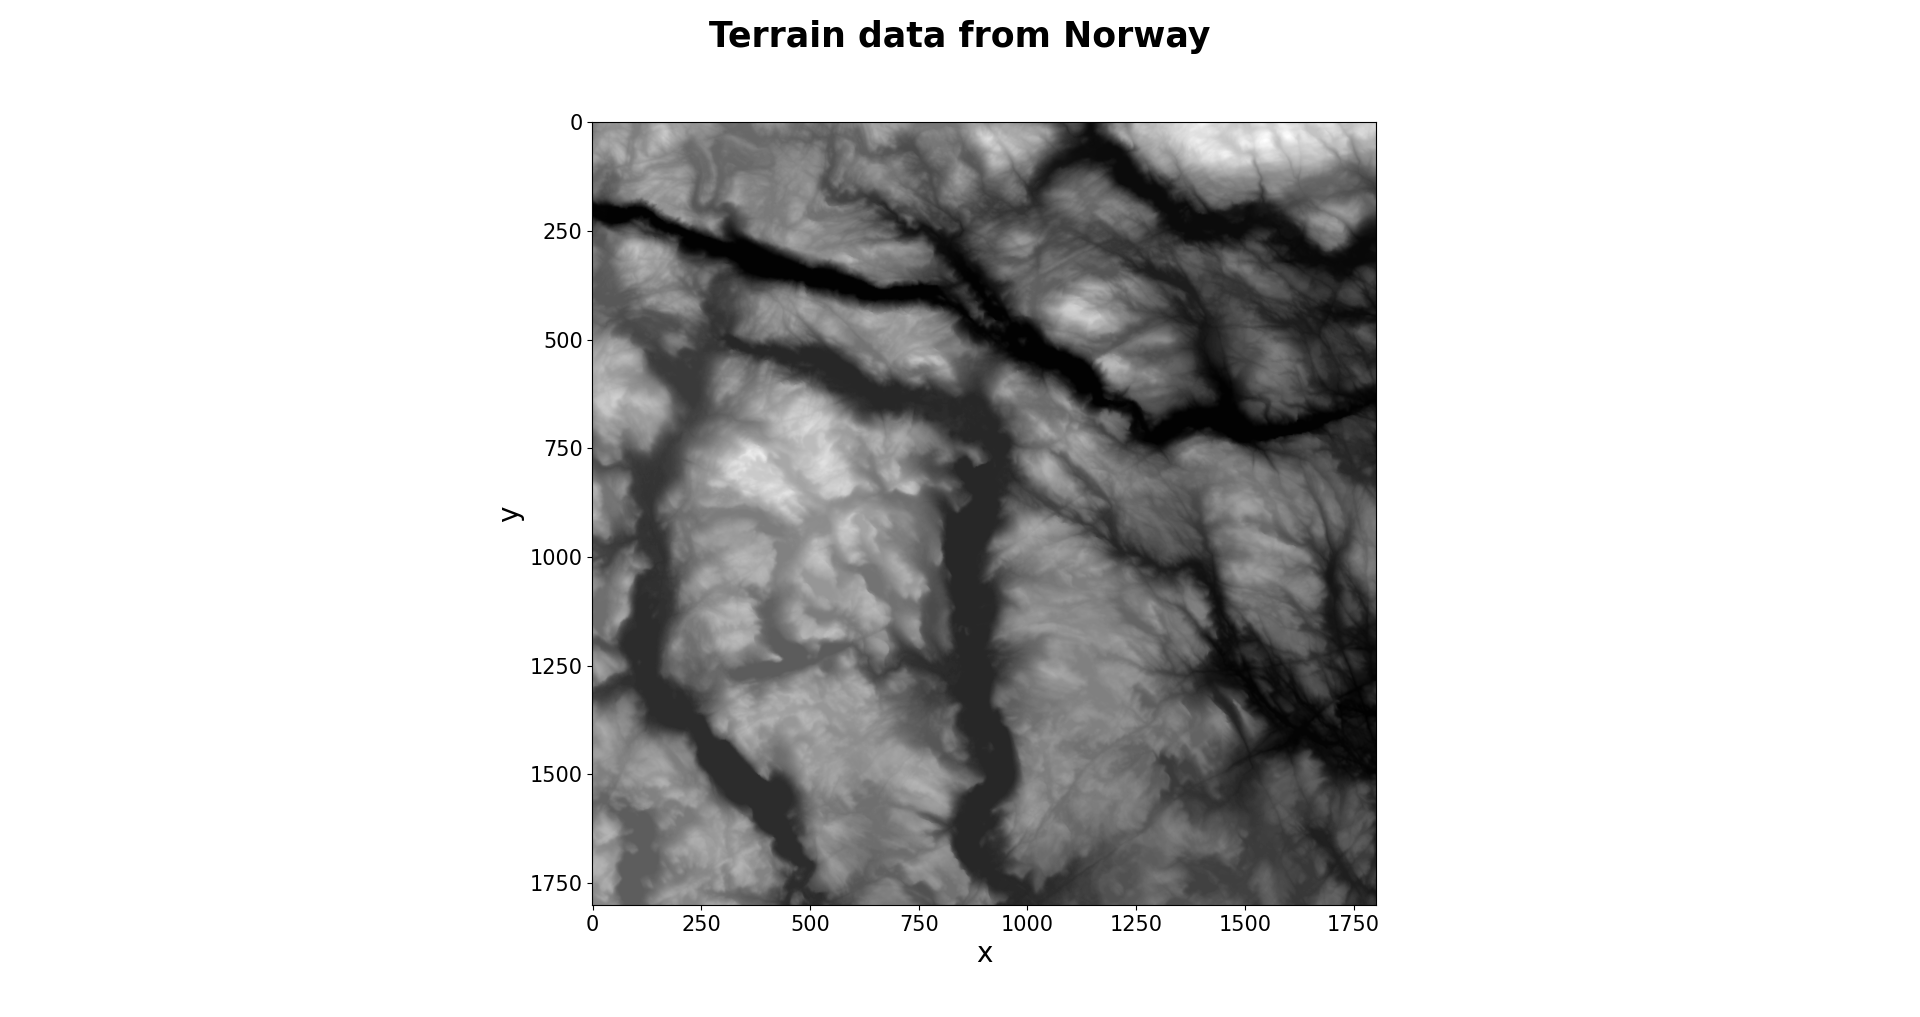
\includegraphics[width = 1\linewidth]{C:/Users/Sander/Documents/GitHub/FYS-STK4155/Project1/Report/Figures/terrainData1.PNG}
\caption{\label{fig:terrainData1} Terrain data over Norway.}
\end{figure}

\noindent We also want to scale the data so that the distribution of the data is centred around zero with standard deviation one. Additionally, we only consider every 10th point on figure \ref{fig:terrainData1} for computational effective reasons. Doing this results in figure \ref{fig:terrainData2}

\begin{figure}[H]
\centering
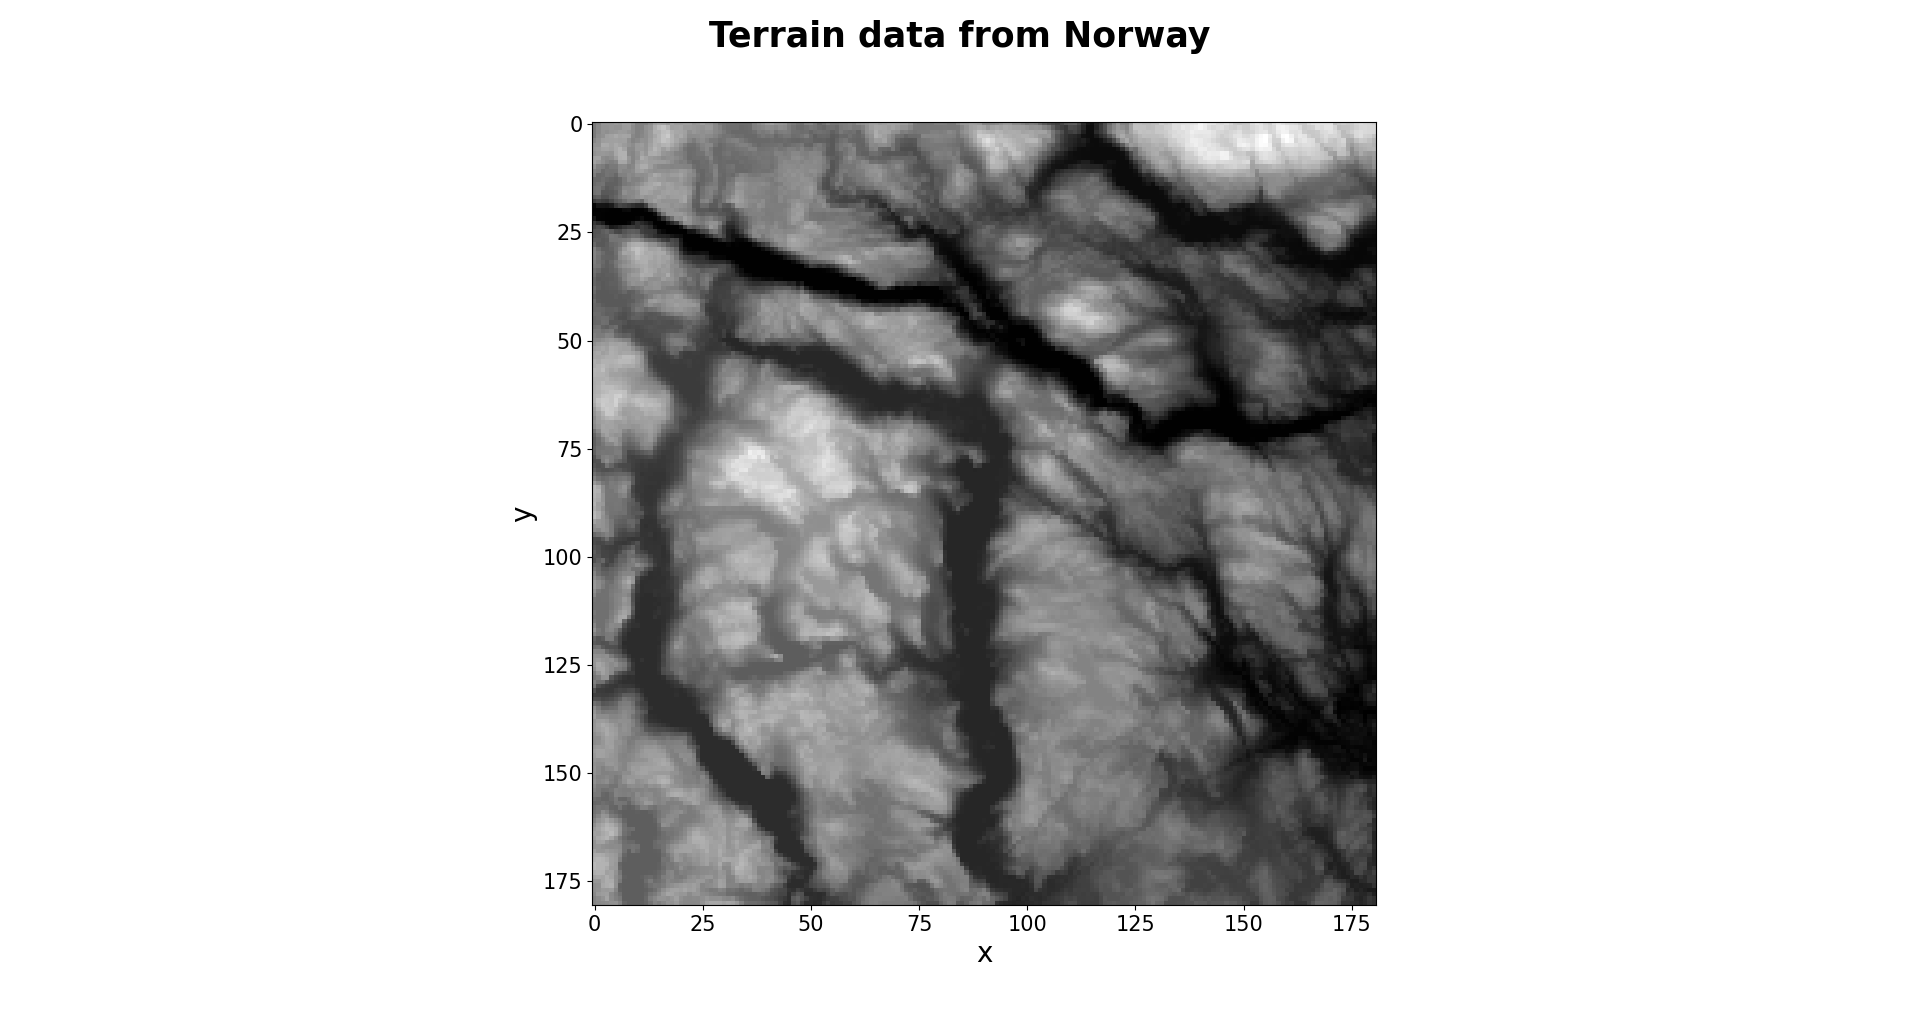
\includegraphics[width = 1\linewidth]{C:/Users/Sander/Documents/GitHub/FYS-STK4155/Project1/Report/Figures/terrainData_clip_scale_skip.PNG}
\caption{\label{fig:terrainData2} Terrain data over Norway where the data has been scaled and reduced to $\frac{n}{10}$ data points.}
\end{figure}

\noindent Figure \ref{fig:terrainData2} will from now act as the response $\hat{y}$ just like the Franke function have been used so far. Since we have already developed the tools to model the image in figure \ref{fig:terrainData2}, we can proceed to exercise g.

\newpage

\begin{center}
\Large{\textbf{Exercise 1g) Real data analysis}}
\end{center}

\begin{center}
\large{\textbf{Setting parameters}}
\end{center}

\noindent In this exercise I want to demonstrate how to properly go forth when creating a decent model using linear regression, or in other words, I want to find the optimal parameters of a linear regression model. Three models will be made, one OLS, one Ridge and one Lasso using 10-fold CV. 10-fold CV was chosen as it gave reasonable results in the previous exercises and it shortens the run-time in the python code compared to the LOOCV. Any noise in our model is removed as the noise-level was simply a tool to simulate realistic data. The number of observations is this time determined by the data set (figure \ref{fig:terrainData1}) and is $\frac{1800^2}{10} = 324000$. We can now list a table where we keep our variables updated as we go

\begin{table}[h]
\caption{\label{tab:update1} An overview of the three models which will be updated as we go. Undiscovered parameters/values are denoted by "-".}
\centering
\begin{tabular}{c|c|c|c}
 & OLS & Ridge & Lasso\\
\hline
Number of observation n & $324000$ & $324000$ & $324000$\\
\hline
noise-level & $0$ & $0$ & $0$\\
\hline
Optimal $\lambda$ & None & - & -\\
\hline
Optimal complexity p & - & - & -\\
\hline
Lowest MSE & - & - & -\\
\end{tabular}
\end{table}

\noindent We will continuously update table \ref{tab:update1} as we find the optimal parameters of the three models. This will allow us to better compare the models at the very end to see which one is preferable over the others. 

\begin{center}
\large{\textbf{Finding optimal parameters}}
\end{center}

\noindent Let us first find the optimal values of the shrinkage parameter $\lambda$ for both the Ridge and Lasso regression schemes (OLS does use a shrinkage parameter). We only consider $\lambda$-values in the interval $[0.00001,0.0001,0.001,0.01,0.1]$. Any higher values and most regression coefficients will be reduced towards/to zero, and any lower will just be close to the OLS. We can now plot the MSE as function of polynomial degree using 10-fold CV for the OLS, Ridge and Lasso regression schemes using the array of $\lambda$-values previously mentioned

\begin{figure}[H]
\centering
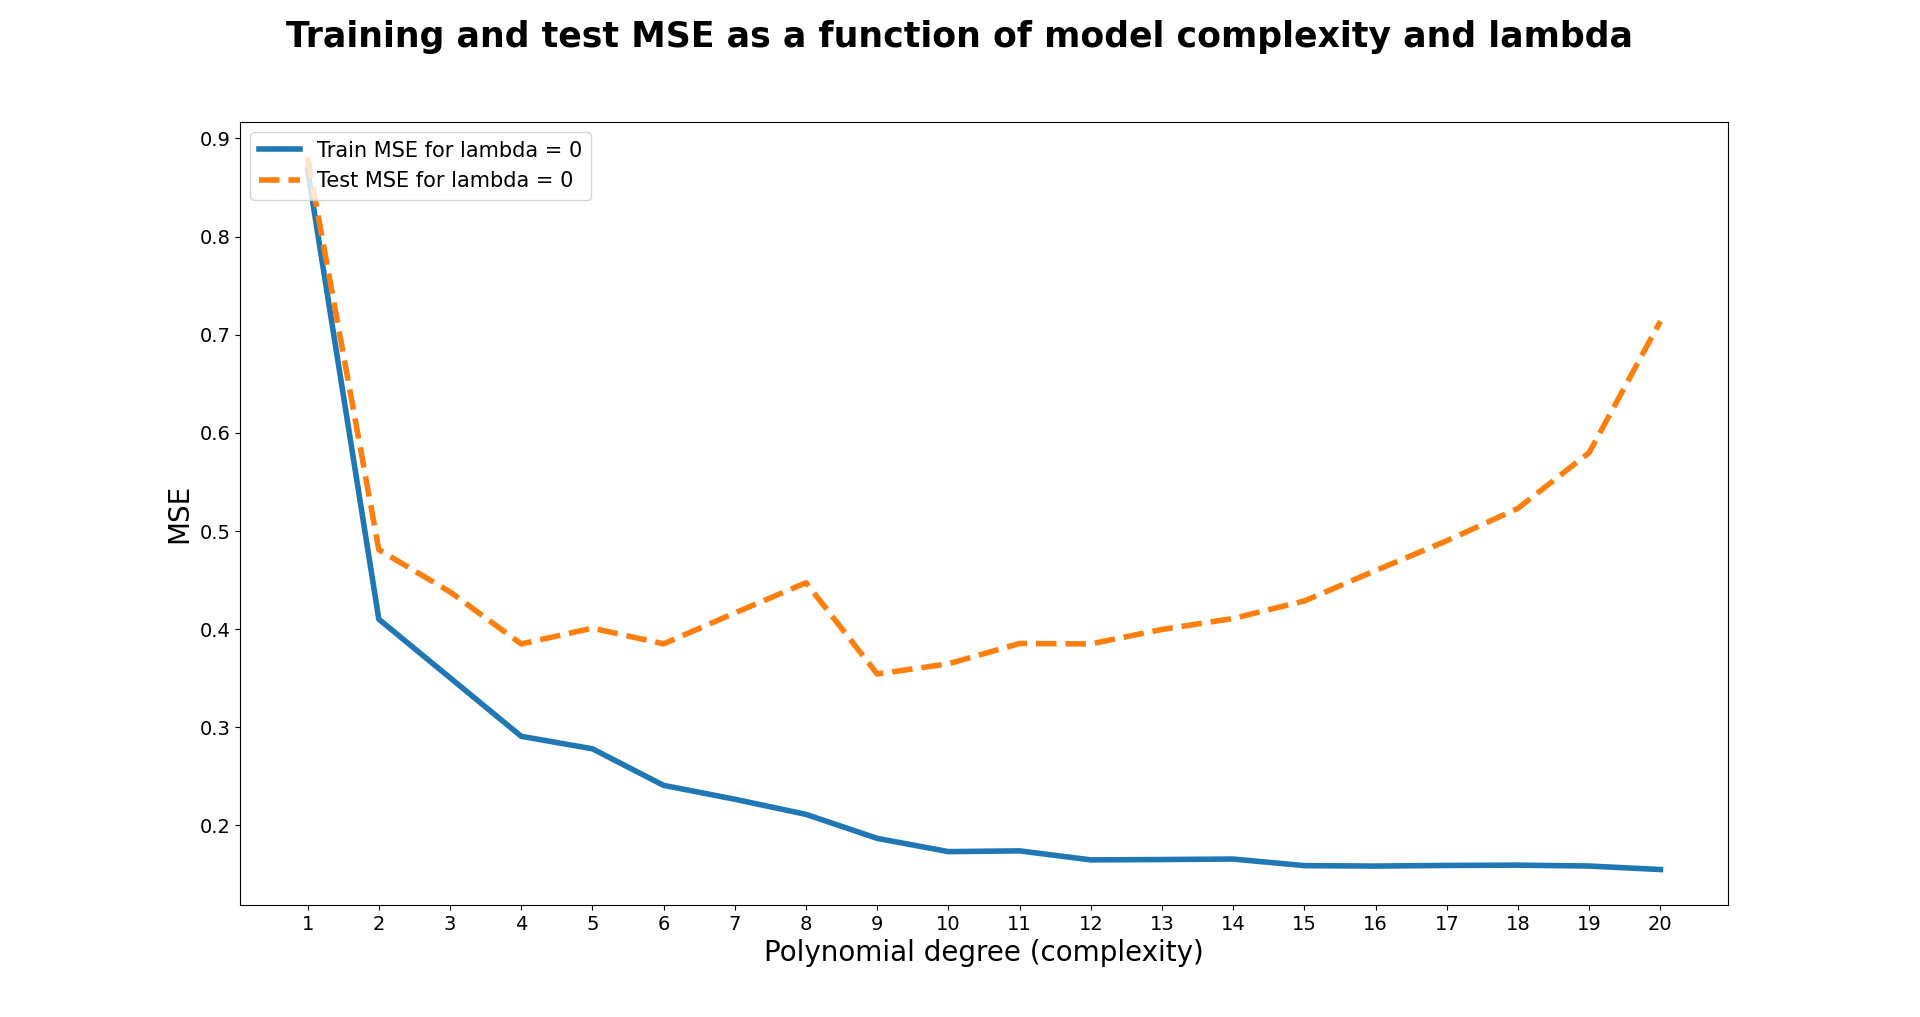
\includegraphics[width = 1\linewidth]{C:/Users/Sander/Documents/GitHub/FYS-STK4155/Project1/Report/Figures/MSECV_p20_CV10_OLS_TERREIN.PNG}
\caption{\label{fig:MSEOLST} MSE as a function of polynomial degree up to 20 using the 10-fold CV resampling method and a OLS regression scheme. Here we have 100 observations while we consider every possible permutation of a 10-fold cross-validation.}
\end{figure}

\begin{figure}[H]
\centering
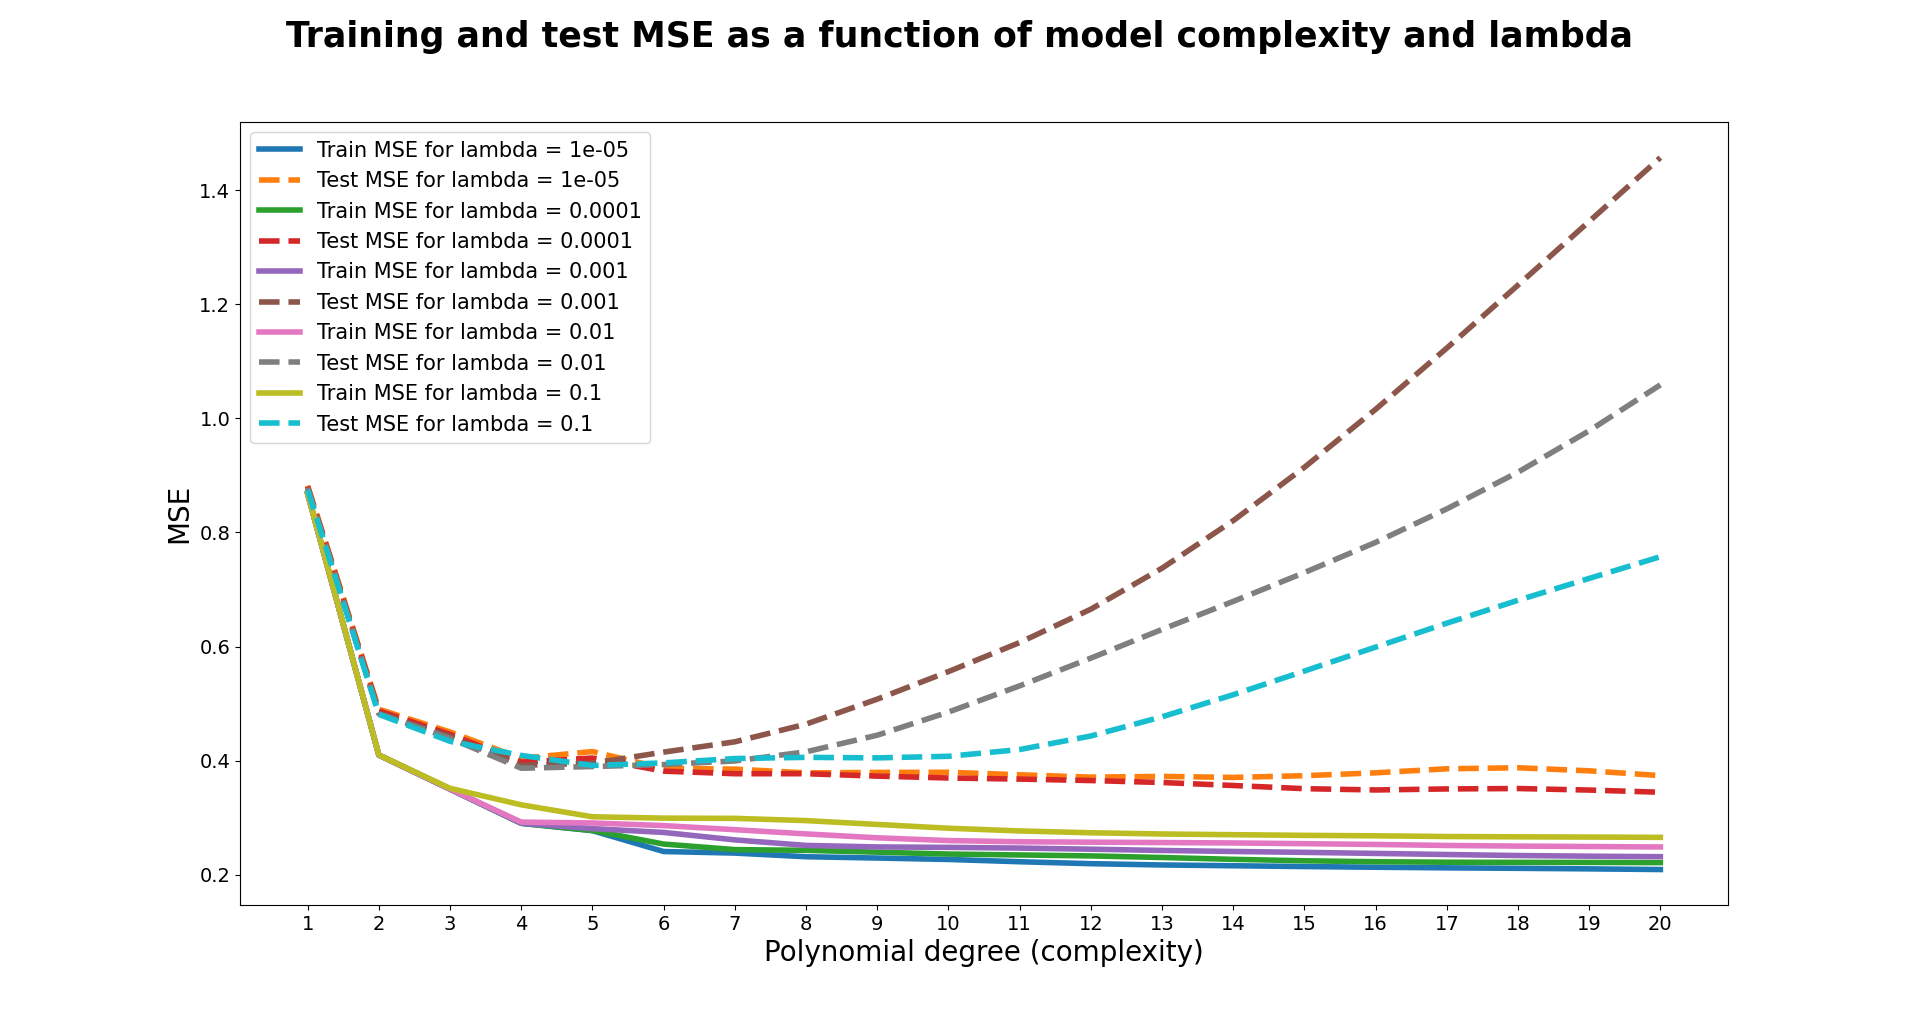
\includegraphics[width = 1\linewidth]{C:/Users/Sander/Documents/GitHub/FYS-STK4155/Project1/Report/Figures/MSECV_p20_CV10_RIDGE_TERREIN.PNG}
\caption{\label{fig:MSERIDGET} MSE as a function of polynomial degree up to 20 for different values of $\lambda$ using the 10-fold CV resampling method and a Ridge regression scheme. Here we have 100 observations while we consider every possible permutation of a 10-fold cross-validation.}
\end{figure}

\begin{figure}[H]
\centering
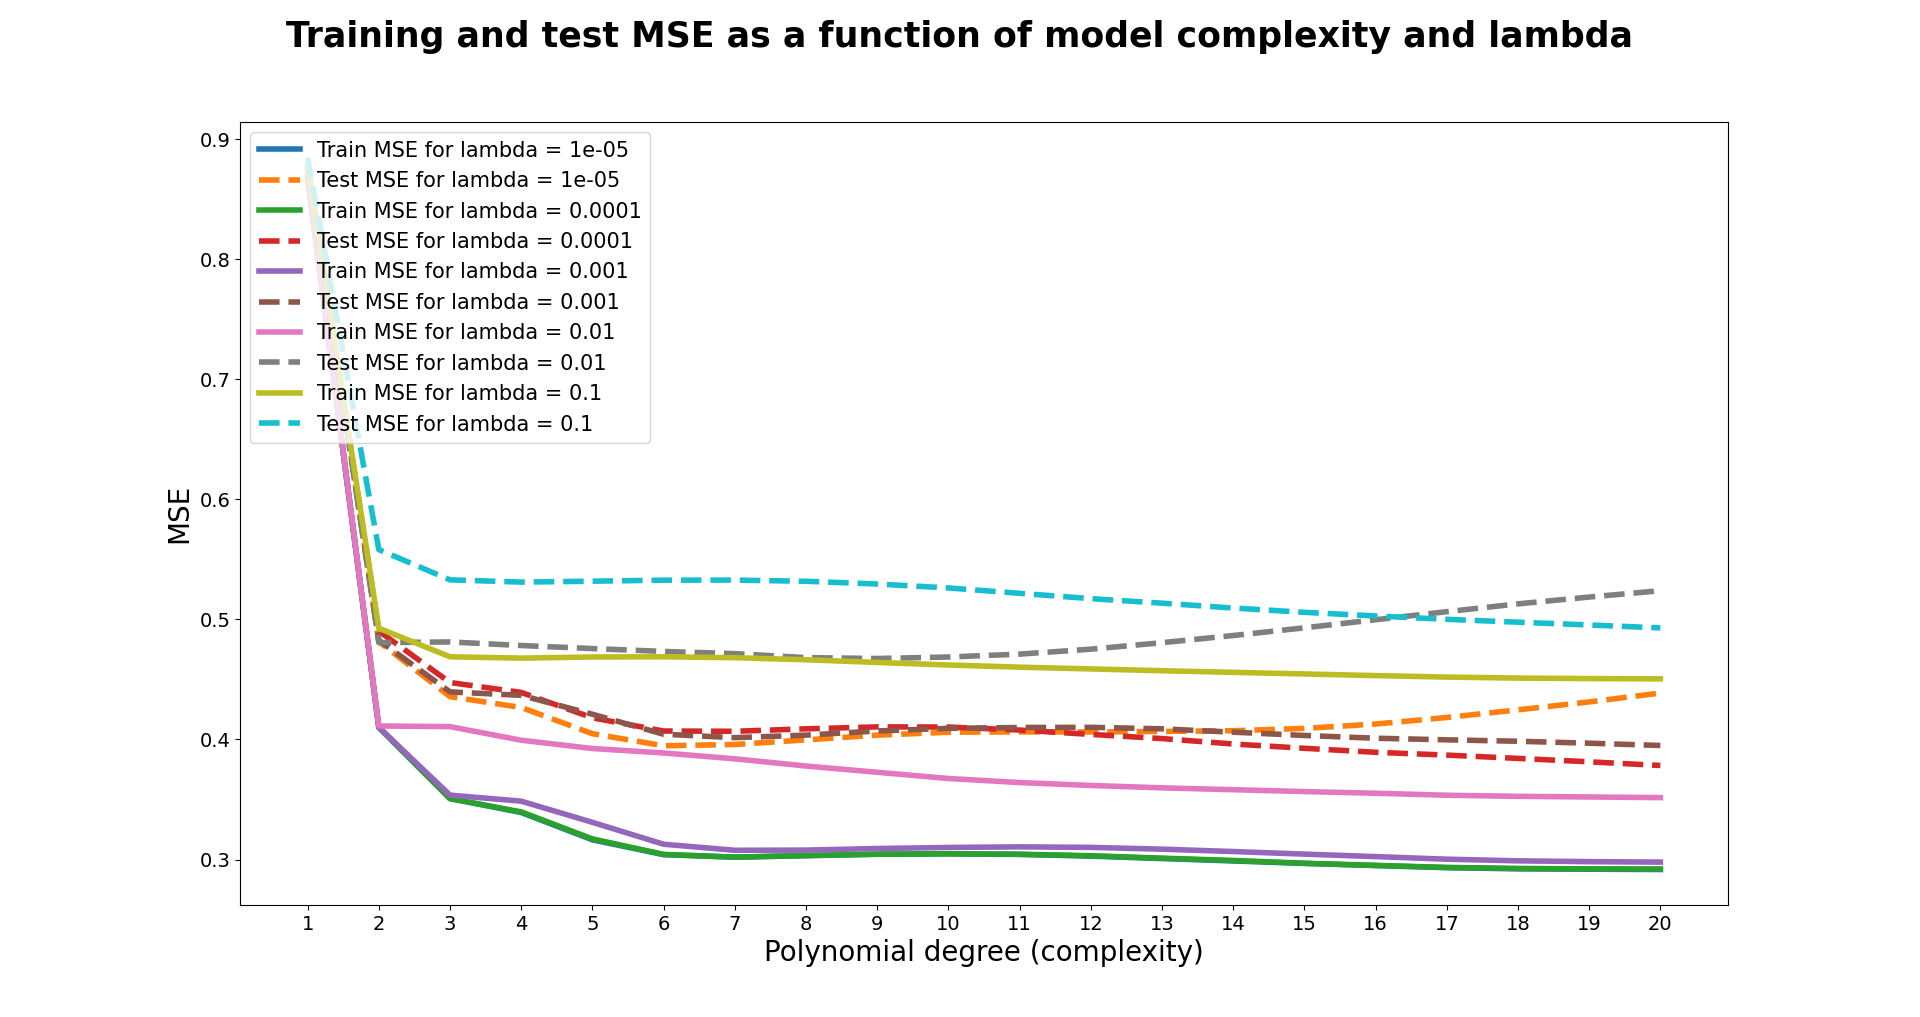
\includegraphics[width = 1\linewidth]{C:/Users/Sander/Documents/GitHub/FYS-STK4155/Project1/Report/Figures/MSECV_p20_CV10_Lasso_TERREIN.PNG}
\caption{\label{fig:MSELASSOT} MSE as a function of polynomial degree up to 20 for different values of $\lambda$ using the 10-fold CV resampling method and a Lasso regression scheme. Here we have 100 observations while we consider every possible permutation of a 10-fold cross-validation.}
\end{figure}

\noindent From figures \ref{fig:MSEOLST}, \ref{fig:MSERIDGET} and \ref{fig:MSELASSOT} we can observe that there are large differences between the three regression schemes. The OLS scheme behaves as normal as the test MSE decreases until some minimum value and then proceeds to sharply increase as over-fitting occurs. The ridge behaves similar to the OLS for $\lambda = 0.1,0.01,0.001$ while the test MSE really never increases for $\lambda = 0.0001,0.00001$. The latter is also how the Lasso models behave as the complexity of the model never seems to increase the test MSE. This may mean that the over-fitting occurs at complexities higher than $p = 20$. With that being said, the test MSE for the Lasso models barely decrease after some point. 
\\
However, we can still find which $\lambda$-value produces the lowest test MSE and at which polynomial degree this occurs for the three regression schemes. These values were found and put into table \ref{tab:update1} and the updated table then looks like

\begin{table}[h]
\caption{\label{tab:update2} An overview of the three models which will be updated as we go. Undiscovered parameters/values are denoted by "-".}
\centering
\begin{tabular}{c|c|c|c}
 & OLS & Ridge & Lasso\\
\hline
Number of observation n & $324000$ & $324000$ & $324000$\\
\hline
noise-level & $0$ & $0$ & $0$\\
\hline
Optimal $\lambda$ & None & $0.0001$ & $0.0001$\\
\hline
Optimal complexity p & $9$ & $20$ & $20$\\
\hline
Lowest MSE & $0.35434928$ & $0.34483905$ & $0.3783378$\\
\end{tabular}
\end{table}

\begin{center}
\large{\textbf{Training a model using optimal parameters and final thoughts}}
\end{center}

\noindent We can observe from table \ref{tab:update2} that all three regression schemes perform pretty well with regards to MSE. However, the Ridge regression scheme seems to perform the best. We can create three models using the optimal parameters and plot the predicted image for each regression scheme as done in figure \ref{fig:predOLST}, \ref{fig:predRIDGET} and \ref{fig:predLASSOT}.

\begin{figure}[H]
\centering
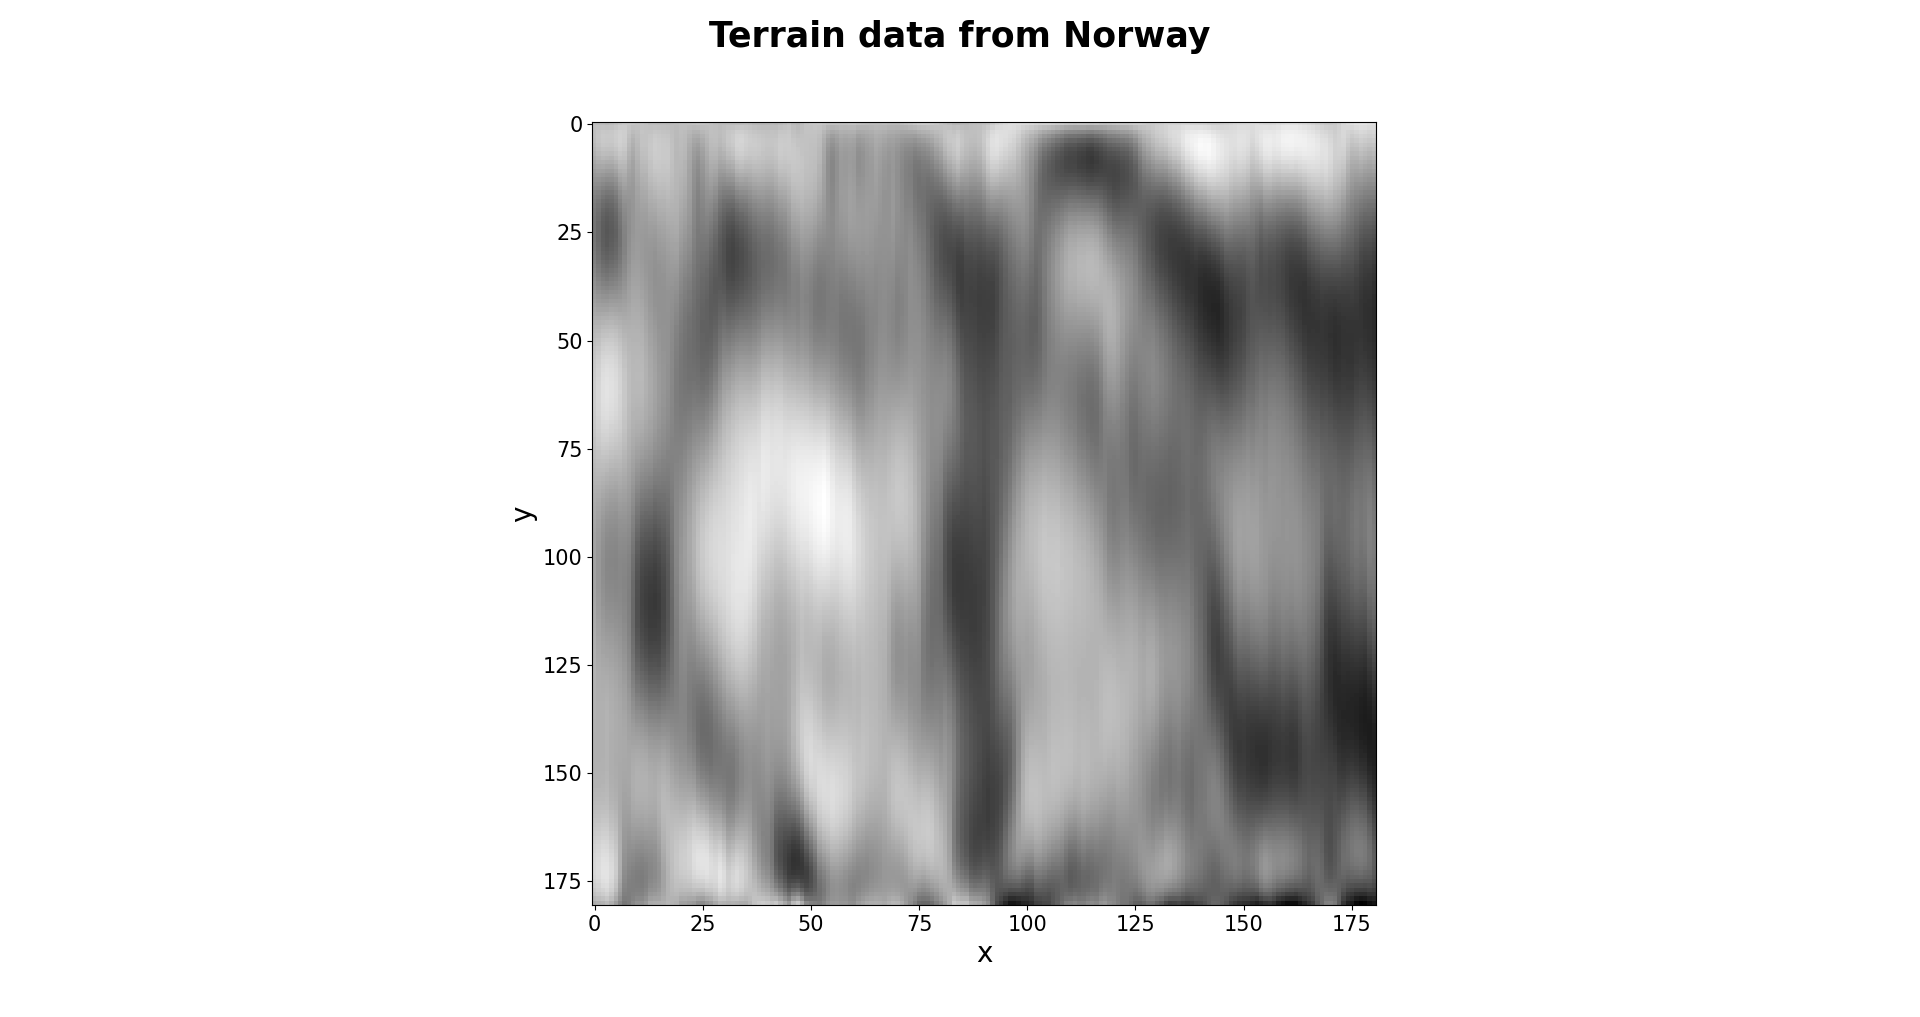
\includegraphics[width = 1\linewidth]{C:/Users/Sander/Documents/GitHub/FYS-STK4155/Project1/Report/Figures/terrainPred_OLS_CV10_p8.PNG}
\caption{\label{fig:predOLST} Final image of the test data using the OLS model based on the optimal parameters in table \ref{tab:update2}.}
\end{figure}

\begin{figure}[H]
\centering
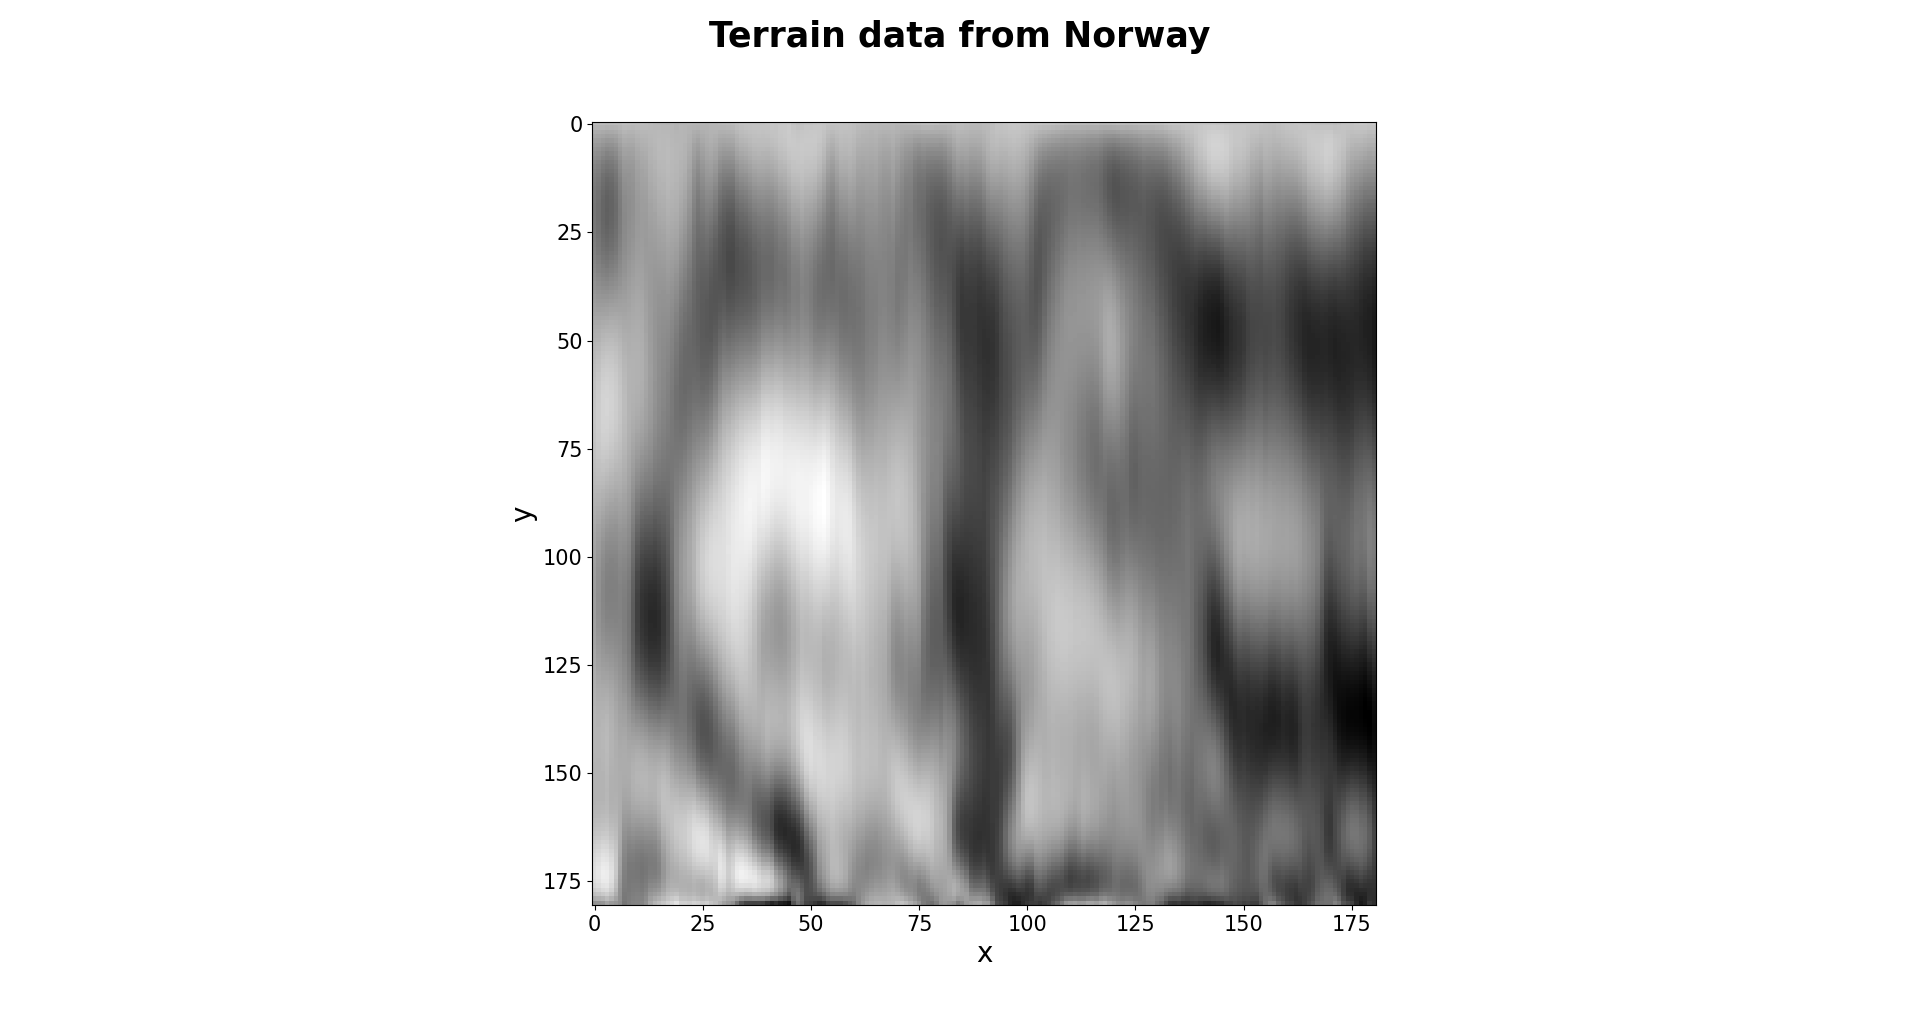
\includegraphics[width = 1\linewidth]{C:/Users/Sander/Documents/GitHub/FYS-STK4155/Project1/Report/Figures/terrainPred_Ridge_CV10_p19_l00001.PNG}
\caption{\label{fig:predRIDGET} Final image of the test data using the Ridge model based on the optimal parameters in table \ref{tab:update2}.}
\end{figure}

\begin{figure}[H]
\centering
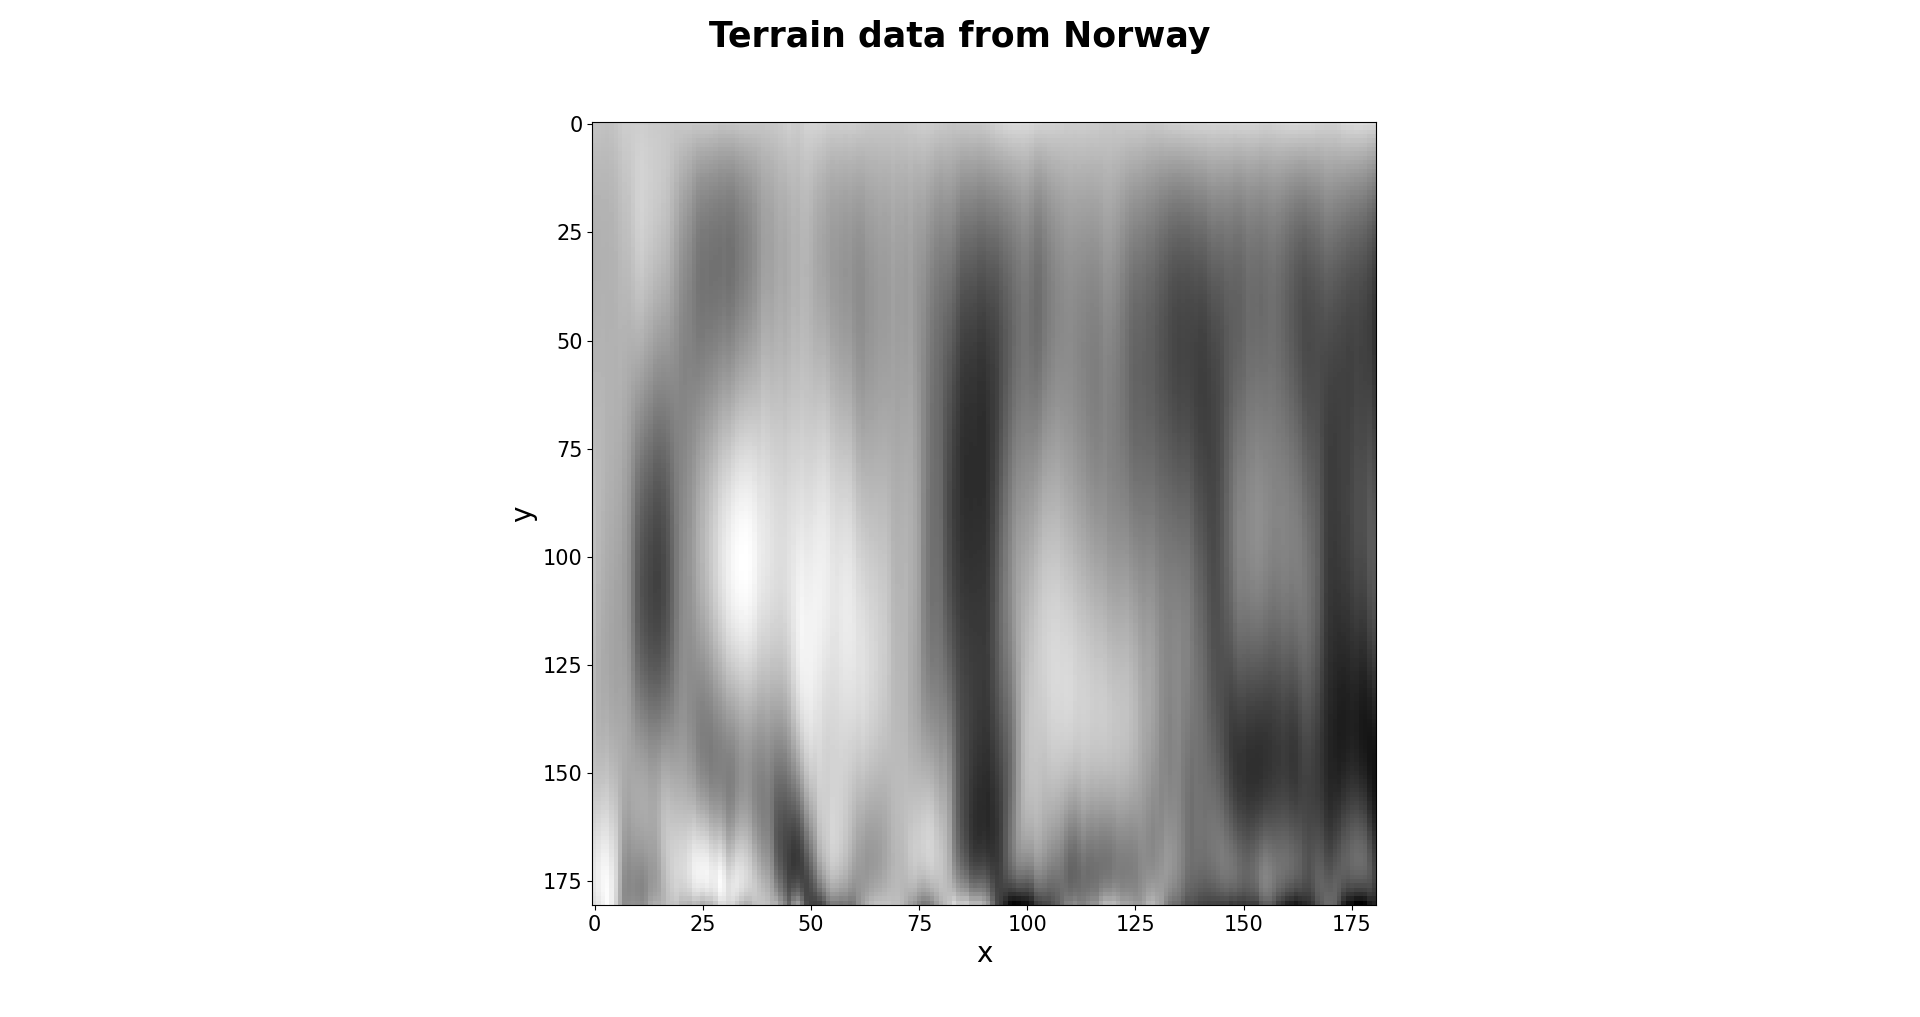
\includegraphics[width = 1\linewidth]{C:/Users/Sander/Documents/GitHub/FYS-STK4155/Project1/Report/Figures/terrainPred_Lasso_CV10_p19_l00001.PNG}
\caption{\label{fig:predLASSOT} Final image of the test data using the Lasso model based on the optimal parameters in table \ref{tab:update2}.}
\end{figure}

\noindent From the test MSE in table \ref{tab:update2} as well as the above images, it seems that Ridge performs the best as figure \ref{fig:predRIDGET} correlates the best with figure \ref{fig:terrainData2}. We can see that the machine learning algorithm is able to capture the main traits of the original image, but severely lacks details. One can see the two vertical "branches" pretty well, and also the smaller "branches" in the lower right corner. However, the two contrasting horizontal "branches" are not well observed in figure \ref{fig:predRIDGET}. 

\newpage

\begin{center}
\Large{\textbf{Conclusion}}
\end{center}

\noindent Basic machine learning algorithms were developed in the form of both bootstrap and CV resampling methods and different regression schemes including OLS, Ridge and Lasso. These algorithms were first used to successfully predict the Franke function where a polynomial degree of 5 yielded the best result when utilizing OLS. The optimal model complexity varied with the Ridge and Lasso regressions depending on what shrinkage parameter $\lambda$ were applied. It was found that smaller values of $\lambda$ (closer to zero) yielded higher MSE when utilizing the bootstrap resampling method, while smaller $\lambda$-values yielded lower MSE when utilizing cross-validation. It was also found that the test MSE for some values of $\lambda$ never really increased with model complexity, meaning the model complexity could be increased without over-fitting. 
\\
The same machine learning algorithms were then used to predict real terrain data. It was found that the Ridge regression performed the best out of the three regression schemes as it had the lowest test MSE. It was found here that over-fitting did not occur for the Lasso and Ridge regression schemes for polynomials less than 20 degrees. However, the OLS did over-fit the data at polynomial degree 9. 
\\
Although the algorithms were able to capture the large overarching traits of the terrain data, the details of the image were outside the capabilities of the algorithms. Still, as this is my first time developing any machine learning algorithm, I consider the predictive capabilities of the algorithm a great success. 

\newpage

\begin{center}
\Large{\textbf{Future work}}
\end{center}

\noindent As previously mentioned, this is my first attempt as developing any machine learning algorithms and thus there are immense room for improvements in several areas. There are probably countless machine learning algorithms out there that can outperform mine, so the first steps to improving my own algorithm should be to "look at the competition" and see where my algorithm falls short.
\\
Algorithms like the one in Scikit-Learn probably implements other fancy stuff into their algorithms which I have neglected or didn't know about. The second step would then be to learn about these fancy things and implement them into my own algorithm to see if it improves the test scores. 
\\
Additionally, my algorithm could also include other regression schemes such as the elastic net, group lasso and fused lasso to see if these would perform better than the regression schemes used in this project.

\newpage

\begin{center}
\Large{\textbf{References}}
\end{center}

\begin{itemize}
  \item Fahrmeir, L., Kneib, T., Lang, S., Marx, B., 2013, \emph{Regression, Models, Methods and Applications}, Springer-Verlag Berlin Heidelberg, pp. 120, DOI: 10.1007/978-3-642-34333-9
  \item Hastie, T., Tibshirani, R., Friedman, J., 2009, [A], \emph{The Elements of Statistical Learning, Data Mining, Inference, and Prediction}, Second edition, Springer Science + Business Media, Inc., pp. 44-45, DOI: 10.1007/b94608
  \item Hastie, T., Tibshirani, R., Friedman, J., 2009, [B], \emph{The Elements of Statistical Learning, Data Mining, Inference, and Prediction}, Second edition, Springer Science + Business Media, Inc., pp. 63-64, DOI: 10.1007/b94608
  \item Hastie, T., Tibshirani, R., Friedman, J., 2009, [C], \emph{The Elements of Statistical Learning, Data Mining, Inference, and Prediction}, Second edition, Springer Science + Business Media, Inc., pp. 68, DOI: 10.1007/b94608
  \item James, G., Witten, D., Hastie, T., Tibshirani, R., 2017, [A], \emph{An Introduction to Statistical Learning, with Applications in R}, Springer Science + Business Media, Inc., pp. 187, DOI: 10.1007/978-1-4614-7138-7
  \item James, G., Witten, D., Hastie, T., Tibshirani, R., 2017, [B], \emph{An Introduction to Statistical Learning, with Applications in R}, Springer Science + Business Media, Inc., pp. 178-181, DOI: 10.1007/978-1-4614-7138-7
  \item Vittinghoff, E., Glidden, D.V., Shiboski, S.C., McCulloch, C.E., 2005, \emph{Regression Methods in Biostatistics, Linear, Logistic, Survival, and Repeated Measures Models}, Springer Science + Business Media, Inc., pp. 137-138, ISBN: 0-387-20275-7
\end{itemize}

\end{document}
